%A classe é a dcc-nce, e o parâmetro a ser informado é diss (para dissertação de mestrado)
\documentclass[diss,english]{dcc-nce}
\usepackage{multirow}
\usepackage{hyperref}
\usepackage{color}
\usepackage{epsfig}
\usepackage{amsthm}
\usepackage{amssymb}
\usepackage{amsmath}
\usepackage{amscd}
\usepackage[brazilian]{babel}
%\usepackage[utf8]{inputenc}
\usepackage{float}
\usepackage{algpseudocode}
\usepackage{subfig}
\usepackage{listings}
\usepackage{bm}
\usepackage{csquotes}
\usepackage{float}
\usepackage{caption}

\newfloat{Algorithm}{t}{lop}
\captionsetup[Algorithm]{labelformat=default}

\definecolor{dkgreen}{rgb}{0,0.6,0}
\definecolor{gray}{rgb}{0.5,0.5,0.5}
\definecolor{mauve}{rgb}{0.58,0,0.82}

\makeatletter
\g@addto@macro{\normalsize}{%
	\setlength{\abovedisplayskip}{5pt}
	\setlength{\abovedisplayshortskip}{5pt}
	\setlength{\belowdisplayskip}{5pt}
	\setlength{\belowdisplayshortskip}{5pt}}
\makeatother

\algnewcommand{\LineComment}[1]{\State \(\triangleright\) #1}
% Para contagem do numero total de folhas:
\usepackage{everyshi}
\makeatletter
\let\totalpages\relax
\newcounter{mypage}
\EveryShipout{\stepcounter{mypage}}
\AtEndDocument{\clearpage
   \immediate\write\@auxout{%
    \string\gdef\string\totalpages{\themypage}}}
\makeatother


\topmargin=0in
\textheight=20.5cm

\def  \R   {{\mathbb R}}
\def  \Z   {{\mathbb Z}}
%\def  \N   {{\mathbb N}}
\def  \Q   {{\mathbb Q}}
\def \Ev {{\mathbb E}}
\def \Pr {{\mathbb P}}
\def \f {{\mathbf f}}
\def \u {{\mathbf u}}
\def \y {{\mathbf y}}
\def \x {{\mathbf x}}
\def \m {{\mathbf m}}
\def \gu {{\bar{g}}}

\newcommand{\Var}{\mathrm{Var}}
\newcommand{\Cov}{\mathrm{Cov}}

\DeclareMathOperator*{\argmax}{arg\,max}
\DeclareMathOperator*{\argmin}{arg\,min}
\begin{document}

\lstset{frame=tb,
	language=Python,
	aboveskip=3mm,
	belowskip=3mm,
	showstringspaces=false,
	columns=flexible,
	basicstyle={\small\ttfamily},
	numbers=none,
	numberstyle=\tiny\color{gray},
	keywordstyle=\color{blue},
	commentstyle=\color{dkgreen},
	stringstyle=\color{mauve},
	breaklines=true,
	breakatwhitespace=true,
	tabsize=3
}

\newtheorem {Theorem}  {Theorem}

\numberwithin{Theorem}{section}

\newtheorem {Lemma}[Theorem]  {Lemma}
\newtheorem {Proposition}[Theorem]{Proposition}
\theoremstyle{definition}
\newtheorem{Definition}[Theorem]{Definition}
\theoremstyle{remark}
\newtheorem{Remark}[Theorem]{Comentário}
\newtheorem{Example}[Theorem]{Example}
\newtheorem {Exercise}[Theorem]{Exercise}
\newtheorem {Corollary}[Theorem]{Corolário}
\newtheorem{Claim}[Theorem]{Claim}
\newtheorem{Assumption}[Theorem]{Assumption}
%Este tem que vir primeiro neste arquivo, caso contrario nao aparecerao
%as palavras-chave na ficha catalografica:
%\keyword{Inferência Bayesiana}
\keyword{Inferência variacional}
\keyword{Processos Gaussianos}

\cip{}


    % Editar o arquivo palavrasChavePortugues

%O restante vem depois:
%\title{Boosted Variational Inference via Bayesian Monte Carlo}

% COLOCAR AQUI O CUTTER (CÓDIGO FORNECIDO PELA BIBLIOTECA DO NCE PARA A FICHA CATALOGRÁFICA):
\codigobiblioteca{CBIB}

\author{Naiff}{Danilo de Freitas}
\advisor[Prof.~Dr.~]{Ramos (DMA - IM-UFRJ)}{Fabio Antônio Tavares Ramos}
\banca{Dr. Yuri Fahham Saporito (EMAP - FGV)}{Dr. Amaro Gomes Barreto Junior (Escola de Química - UFRJ)}{Prof. Dr. Hugo Tremonte de Carvalho (DME - IM-UFRJ)}{Dr. Adriano Mauricio de Almeida Cortes (UFRJ Xerem)}
\date{2019}
\maketitle
                      % Editar o arquivo capa.tex
%\pagenumbering{roman} %numeração de páginas em romano começa a partir do primeiro capítulo

\clearpage

\mbox{}\vfill

\begin{flushright}

{\sffamily\itshape

Aqui coloque a dedicatória...

Se não houver, delete esta parte.

}

\end{flushright}
               % Editar o arquivo dedicatoria.tex
%\begin{agradecimentos}
Coloque aqui os agradecimentos.

Agradeço aos meus pais, meu orientador, à bolsa, etc...
\end{agradecimentos}
            % Editar o arquivo agradecimentos.tex
%\begin{abstract}

%MADUREIRA, Rodrigo Lopes Rangel. Algoritmos de interseções, bla bla bla...\\

Inferência Bayesiana é um dos paradigmas principais da Estatística, um que nos ultimos anos se mostrou bem sucedido. Porém, várias técnicas para ele requer um numero grande de avaliações de \textit{posterioris}, o que pode ser inviável em algumas aplicações. Baseado em trabalhos pré-existentes, um novo algorítmo de inferencia aproximada é desenvolvido neste trabalho, baseado em inferência variacional e processos Gaussianos. Esse algorítmo, nomeado pelo autor Boosted Variational Bayesian Monte Carlo, é desenvolvido para que poucas avaliações de \textit{posteriori} sejam necessárias. O algorítmo, a teoria por trás dele, e seu pacote associado são apresentados, sendo aplicado em um número de exemplos.

\end{abstract}
           % Editar o arquivo resumoPortugues.tex
%%\begin{englishabstract}{Colocar aqui o título da dissertação em inglês}{coloque aqui as palavras-chave em inglês, separadas por vírgula}

\begin{englishabstract}{}{Bayesian inference, variational inference, Gaussian processes, Bayesian Monte Carlo}


%MADUREIRA, Rodrigo Lopes Rangel. Algoritmos de interseções, bla bla bla...\\

Most of the important problems in machine learning are computationally expensive, in particular the ones involving Bayesian inference. Many of the current Bayesian techniques requires a large number of likelihood evaluations, which may be infeasible for some cases. In this dissertation, we propose an approximate inference algorithm, based on recent works on variational inference and Gaussian processes. This algorithm, named by the author Boosted Variational Bayesian Monte Carlo, is designed so that few likelihood evaluations are needed. The algorithm, its associated package, and the theory behind it are presented in this work. We also illustrate the algorithm by implementing it in some toy examples, and in a contamination source problem.

\end{englishabstract}

              % Editar o arquivo resumoIngles.tex
\thispagestyle{empty} \begin{center} {\bf {\Large Universidade
Federal do Rio de Janeiro}}
\bigskip
\bigskip
\bigskip
\bigskip
\bigskip

{\bf {\LARGE{\emph {Boosted Variational Inference via Bayesian Monte Carlo}}}}
\bigskip
\bigskip
\bigskip
\bigskip

{\bf{Danilo de Freitas Naiff}}

\bigskip
\bigskip
\bigskip
\bigskip
\bigskip
\bigskip
\bigskip
\bigskip
\bigskip
\bigskip
\bigskip
\bigskip
\bigskip
\bigskip
\bigskip
\bigskip
\bigskip
\bigskip
\bigskip
\bigskip
\bigskip
\bigskip
\bigskip
\bigskip
\bigskip
\bigskip
\bigskip
\bigskip
\bigskip
\bigskip
\bigskip
\bigskip
\bigskip
\bigskip
\bigskip
\bigskip
\bigskip
\bigskip
\bigskip

{\large \bf {Rio de Janeiro}}

\bigskip

{\large \bf{Setembro de 2019}}
\end{center}

\newpage
%\thispagestyle{empty}
\pagenumbering{roman}

\begin{center}
{\bf {\Large Universidade Federal do Rio de Janeiro}}
\end{center}
\bigskip
\bigskip

\begin{center}
 {\Large{\emph {Boosted Variational Inference via Bayesian Monte Carlo}}}
\bigskip
\bigskip
\\
{Danilo de Freitas Naiff}
\end{center}

\bigskip
\bigskip
\bigskip

Disserta{\c c}\~{a}o de Mestrado apresentada ao Programa de P{\'o}s-gradua{\c c}\~{a}o
em Matem{\'a}tica, Instituto de Matem{\'a}tica, da Universidade
Federal do Rio de Janeiro (UFRJ), como parte dos requisitos
necess{\'a}rios {\`a} obten{\c c}\~{a}o do t{\'i}tulo de Mestre em Matem{\'a}tica.

\bigskip

\noindent Orientador: Prof. Fabio Ant\^onio Tavares Ramos.

\bigskip
\bigskip
\bigskip
\bigskip
\bigskip
\bigskip
\bigskip
\bigskip
\bigskip
\bigskip
\bigskip
\bigskip
\bigskip
\bigskip
\bigskip
\bigskip
\bigskip
\bigskip
\bigskip
\bigskip
\bigskip
\bigskip
\bigskip
\bigskip
\bigskip
\bigskip
\bigskip
\bigskip
\bigskip


\begin{center}
{\bf  Rio de Janeiro}\\
{\bf  Setembro de 2019}
\end{center}

\newpage
%\thispagestyle{empty}

\begin{center}
{\bf {\Large Universidade Federal do Rio de Janeiro}}
\end{center}
\bigskip
\bigskip

\begin{center}
 {\Large{\emph {Boosted Variational Inference via Bayesian Monte Carlo}}}
\bigskip
\bigskip
\\
{Danilo de Freitas Naiff}
\end{center}

\bigskip
\bigskip
\bigskip

Disserta{\c c}\~{a}o de Mestrado apresentada ao Programa de P{\'o}s-gradua{\c c}\~{a}o
em Matem{\'a}tica, Instituto de Matem{\'a}tica, da Universidade
Federal do Rio de Janeiro (UFRJ), como parte dos requisitos
necess{\'a}rios {\`a} obten{\c c}\~{a}o do t{\'i}tulo de Mestre em Matem{\'a}tica.

{\indent{Aprovada por:}}
\ \\
\ \\

{\indent{-----------------------------------------------------------}}\\
{\indent{Prof. Fabio Ant\^onio Tavares Ramos}\\
\ \\

{\indent{-----------------------------------------------------------}}\\
{\indent{Prof. Heudson Tosta Mirandola} \\
	\ \\
	
{\indent{-----------------------------------------------------------}}\\
{\indent{Prof. Yuri Fahham Saporito} \\
\ \\

{\indent{-----------------------------------------------------------}}\\
{\indent{Prof. Amaro Gomes Barreto Junior} \\
\ \\

{\indent{-----------------------------------------------------------}}\\
{\indent{Prof. Hugo Tremonte de Carvalho} \\
	\ \\

{\indent{-----------------------------------------------------------}}\\
{\indent{Prof. Adriano Mauricio de Almeida Cortes} \\
\ \\



\bigskip
\bigskip
\bigskip
\bigskip
\bigskip

\begin{center}
{\bf Rio de Janeiro}\\
{\bf Setembro de 2019}
\end{center}

\newpage

\begin{tabular}{|p{12cm}|}
\hline
\ \\
\hspace{1cm}Naiff, Danilo de Freitas.\\
\hspace{1.6cm}Boosted Variational Inference via Bayesian Monte\\\hspace{1cm}Carlo/\;Danilo de Freitas Naiff. - Rio de Janeiro:\\\hspace{1cm}UFRJ/\;IM,\;2019.\\
\hspace{1.6cm}xiii,135f.: il.; 29,7 cm.\\
\hspace{1.6cm}Orientador: Fabio Ant\^onio Tavares Ramos.\\
\hspace{1.6cm}Disserta{\c c}\~{a}o (mestrado)\,---\,Universidade Federal do \\ \hspace{1cm}Rio de Janeiro, Instituto de Matem\'atica, Programa de\\ \hspace{1cm}P\'os-Gradua{\c c}\~{a}o em Matem\'atica, 2019.\\
%\hspace{1.6cm}Refer�ncias %Bibliogr�ficas: p. 165-184 .\\
\hspace{1.6cm}Refer\^encias Bibliogr\'aficas: f. 101-114. \\
 \\
\hspace{1.6cm}1. Bayesian Inference. 2. Variational Inference. \\\hspace{1cm}3. Gaussian Processes. 4.\;Bayesian Monte Carlo. I. Ramos, \\\hspace{1cm}Fabio Ant\^onio Tavares. II. Universidade Federal do Rio de\\\hspace{1cm}Janeiro,Programa de P\'os-Gradua{\c c}\~{a}o em Matem\'atica. III.\\\hspace{1cm}T\'itulo.\\
\hline
\end{tabular}

\newpage

\ \\
\vspace{4cm}

\begin{center}
Dedicado a Ronaldo Lemos Naiff.\\
\end{center}

\newpage

\begin{center}
{\bf{\large Acknowledgments}}
\end{center}
\bigskip

\textit{The following acknowledgments are written in portuguese}

\bigskip
Agrade{\c c}o ao meu orientador F\'abio, que me deu o apoio e conhecimento necess\'ario para desenvolver esse trabalho. Agrade{\c c}o ao pessoal do LABMA, pelo companheirismo e pelas ideias que me deram. Agrade{\c c}o aos meus colegas e \`a equipe do FMTC, competi{\c c}\~ao que me ensinou muitas coisas, algumas usadas neste trabalho. De forma mais abstrata, existe toda uma comunidade que permite que id\'eias possam ser compartilhadas, e implementadas, com uma facilidade muito maior do que se teria em d\'ecadas passadas, e eu agrade{\c c}o a ela.

Agrade{\c c}o a todos os amigos que me deram suporte por todos esses anos. Em particular, aqueles que me ouviram falando sobre meus estresses durante a escrita deste texto, sobre problemas em que seus pontos de vista eram absurdamente abstratos. Agrade{\c c}o a minha m\~ae Rose, pelo suporte durante esse tempo, assim como ao meu av\^o Reinaldo. Finalmente, agrade{\c c}o ao meu pai Ronaldo, que nunca imaginaria que eu acabaria por fazer um mestrado em Matem\'atica, mas que acho que n\~ao ficaria triste com isso.

Finalmente, este \'e um trabalho financiado por ag\^encias p\'ublicas, o que no final \'e dinheiro de um povo sofrido, que em sua maioria ganha muito menos do que o que me foi oferecido. Agrade{\c c}o a este, e espero que o ganho total que possa dar de volta justifique este investimento.



\begin{flushright}
Danilo de Freitas Naiff\\
Setembro de 2019
\end{flushright}

\newpage
\begin{center}
{\bf {\large Resumo}}
\end{center}
\bigskip


\begin{center}
 {\large{\emph {Boosted Variational Inference via Bayesian Monte Carlo\\}}}
\bigskip
\bigskip
{Danilo de Freitas Naiff}
\end{center}

\bigskip

Resumo da disserta{\c c}\~{a}o de Mestrado apresentada ao Programa de P{\'o}s-gradua{\c c}\~{a}o
em Matem{\'a}tica, Instituto de Matem{\'a}tica, da Universidade
Federal do Rio de Janeiro (UFRJ), como parte dos requisitos
necess{\'a}rios {\`a} obten{\c c}\~{a}o do t{\'i}tulo de Mestre em Matem{\'a}tica.


\bigskip

\begin{quote}
{\bf \emph{Resumo:}} A maioria dos problemas importantes em aprendizado de m\'aquina s\~ao caros computacionalmente, em particular aqueles que envolvem infer\^encia Bayesiana. Muitas das t\'ecnicas Bayesianas atuais requerem um alto n\'umero de avalia{\c c}\~oes de verossimilhan{\c c}a, o que pode ser invi\'avel em alguns casos. Nessa disserta{\c c}\~ao, propomos um algoritmo de infer\^encia aproximada, baseado em trabalhos recentes sobre infer\^encia variacional e processos Gaussianos. Este algor\'itmo, nomeado pelo autor \textit{Boosted Variational Bayesian Monte Carlo}, \'e construido de forma que poucas avalia{\c c}\~oes de verossimilhan{\c c}a sejam necess\'arias. O algoritmo, seu pacote associado, e a teoria por tr\'as dele s\~ao apresentados neste trabalho. Tambem ilustramos o algoritmo atrav\'es de sua implementa{\c c}\~ao em alguns \textit{toy examples}, e em um problema de fonte de contamina{\c c}\~ao.

\end{quote}



\bigskip

\noindent{\bf{Palavras--chave.}} Infer\^encia Bayesiana, Infer\^encia variacional, Processos gaussianos, Bayesian Monte Carlo.

\bigskip
\bigskip
\bigskip
\bigskip
\bigskip
\bigskip
\bigskip
\bigskip
\bigskip
\bigskip
\bigskip

\ \\
\begin{center}
{\bf \large Rio de Janeiro}\\
{\bf \large Setembro de 2019}
\end{center}

\newpage

\begin{center}
{\bf {\large {\emph {Abstract}}}}
\end{center}
\bigskip

\begin{center}
 {\large{\emph {Boosted Variational Inference via Bayesian Monte Carlo\\}}}
\bigskip
\bigskip
{Danilo de Freitas Naiff}
\end{center}

\bigskip

{\emph {Abstract}} da disserta{\c c}\~{a}o de Mestrado apresentada ao Programa de P{\'o}s-gradua{\c c}\~{a}o
em Matem{\'a}tica, Instituto de Matem{\'a}tica, da Universidade
Federal do Rio de Janeiro (UFRJ), como parte dos requisitos
necess{\'a}rios {\`a} obten{\c c}\~{a}o do t{\'i}tulo de Mestre em Matem{\'a}tica.

\bigskip

\begin{quote}
{\bf \emph{Abstract:}} Most of the important problems in machine learning are computationally expensive, in particular the ones involving Bayesian inference. Many of the current Bayesian techniques requires a large number of likelihood evaluations, which may be infeasible for some cases. In this dissertation, we propose an approximate inference algorithm, based on recent works on variational inference and Gaussian processes. This algorithm, named by the author \textit{Boosted Variational Bayesian Monte Carlo}, is designed so that few likelihood evaluations are needed. The algorithm, its associated package, and the theory behind it are presented in this work. We also illustrate the algorithm by implementing it in some toy examples, and in a contamination source problem.
\end{quote}

\bigskip

\noindent{\bf{Keywords.}} Bayesian inference, variational inference, Gaussian processes, Bayesian Monte Carlo.


\bigskip
\bigskip
\bigskip
\bigskip
\bigskip
\bigskip
\bigskip
\bigskip
\bigskip
\bigskip
\bigskip


\ \\
\begin{center}
{\bf \large Rio de Janeiro}\\
{\bf \large September 2019}
\end{center}

\listoffigures{}

\listoftables{}

%% Examples

\begin{listofabbrv}{XXXXXX}
  \item [BCNF] Boyce Codd Normal Form
  \item [XSLT] XSL Transformations
\end{listofabbrv}
    % Editar o arquivo listaAbreviaturaSiglas.tex

\tableofcontents{}                  % Sumário

\parindent=1.25cm %start for each paragraph from the left margin
\parskip=20pt
\baselineskip=20pt


\chapter{Summary}

\pagenumbering{arabic} %numeração de páginas em arábico começa a partir do primeiro capítulo

The Bayesian framework for inference and learning is conceptually simple, while having good properties related to normative reasoning \cite{Ghahramani_2015}. However, behind its simplicity lies the computational challenge of sampling and integration, which drives much of research on the field. Methods such as Markov Chain Monte Carlo and variational inference have undergone major advances in the recent decades, driving Bayesian methods back to popularity.

In general those methods assume that evaluation of a likelihood function $l(\theta) = p(\mathcal{D}|\theta)$ is computationally cheap enough to be done tens or hundred thousand of times, at least. However, in some cases this may not be true, as for example in cases where $l(\theta)$ must come from a computationally expensive simulation. This work presents a variational approximation method, using Gaussian process regression, that is adapted from \cite{Acerbi_2018,Guo_2016}, in order to deal with cases where $\theta$ is a continuous random variable, and $l(\theta)$ can be evaluated only tens, hundreds, or thousands of times. The current algorithm is suited for low and medium dimensional problems (around 10 dimensions at most).

A Python package for deploying this method was developed, built mainly on top of PyTorch, and we test it in some cases. Currently, the package lacks complete documentation and unit testing, but an alpha version is already available in \url{https://github.com/DFNaiff/BVBMC}. Since this package may undergo changes in the future, all code used in the present work may be found in \url{https://github.com/DFNaiff/Dissertation}.

Next, we presented a brief summary of each chapter of this dissertation.

In Chapter 2, Bayesian theory is briefly reviewed, along with some approximate inference methods. Moreover, approaches to expensive or intractable likelihoods are discussed.

In Chapter 3, the Gaussian process regression method is reviewed, while in Chapter 4, Bayesian Monte Carlo, a Gaussian process based integration method, is discussed.

In Chapter 5, variational inference is reviewed, first in general, then focusing on the case where approximation is made by mixtures of Gaussian distributions, using the boosting approach found in \cite{Guo_2016}. Moreover, a recent method presented in \cite{Acerbi_2018}, using variational inference via Bayesian Monte Carlo, called Variational Bayesian Monte Carlo, is presented.

In Chapter 6, we propose an adaptation of Variational Bayesian Monte Carlo, incorporating other ideas presented in chapter 2 and 3, particularly the boosting approach in \cite{Guo_2016}. This results in a new algorithm, which we call Boosted Variational Bayesian Monte Carlo. A small discussion on implementation follows, focused on backpropagation, which is the reason the developed package was built on PyTorch. In Chapter 7, the corresponding Python package is applied in a few toy examples, and in a contamination source problem.

The work is concluded in Chapter 8, where we discuss future directions for both scaling the presented method to higher dimension and to increase its accuracy. In the appendix, among other things, there is an extended discussion on Sparse Gaussian Process, a technique that the author tried to use in order to extend the present method to higher dimensions and greater number of evaluations, although with limited success.         % Editar o arquivo introducao.tex
\chapter{Bayesian inference and learning}

\section{Learning described as Bayesian inference}

The central problem of learning from data can be verbalized as: given that some agent have access to data $\mathcal{D}$, what knowledge can the learner extract from it? One way to approach this problem is by assuming that learning does not take place in a vacuum, but in a world that the learner has uncertain knowledge about, translated into beliefs. The fact that those beliefs are uncertain is important, given that if the learner knew exactly everything he should know about the world, access to data $\mathcal{D}$ could not teach him nothing more.

Given this general framework of "informed uncertainty", one natural way to describe it, mathematically, is by using probability theory for describing the problem. More specifically, it is used the \textit{Bayesian} viewpoint of probability, where degrees of uncertainty about quantities are mapped into probabilities about those \cite{MacKay2003,jaynes03}.

In this interpretation, probability theory does not just deal with random events, but with anything that an agent is uncertain about. So, given some proposition $A$, and given that the learner knows $I$ about the world, $P(A|I)$ represents what he knows about $A$. Thus $A|I$ becomes a random variable, \textit{even if $A$ is not a random event}. Cox's theorem \cite{jaynes03},\cite{Cox_1963} says that, under some certain common sense assumptions about how the learner should ideally reason about beliefs, the rules of probability theory holds, as an extension to logic.

In a simplification of this setting, when learning from the data $\mathcal{D}$, and previous information $I$, the learner must have some set of hypothesis (assuming finite for now) $\mathcal{H} = \{H_1,\ldots,H_t\}$, such that the learner assumes one and only one of then is true, and with each of them associated with a probability $P(H_k)$ such that
\begin{displaymath} 
\sum_{H_k \in \mathcal{H}} P(H_k|I) = 1.
\end{displaymath}
Furthermore, each hypothesis $H_k$ should say something about how likely it is for the data to be generated, given $H_k$ is true, and this information is encoded in $P(\mathcal{D}|H_k,I)$. In this case, Bayes' theorem says that it is possible to obtain the updated probabilities (thus degree of beliefs) $P(H_k|\mathcal{D},I)$ by Bayes' rule:
\begin{equation}\label{bayes_theorem_1}
 P(H_k|\mathcal{D},I) = \frac{P(\mathcal{D}|H_k,I)}{P(\mathcal{D}|I)}P(H_k|I),
\end{equation}
with $p(\mathcal{D}|I)$ being available by marginalization 
\begin{equation}\label{marginalization_1}
 P(\mathcal{D}|I) = \sum_{H_k \in \mathcal{H}} P(\mathcal{D}|H_k,I) P(H_k|I).
\end{equation}

In practice, usually hypothesis does not comes in discrete chunks, but one assumes a \textit{model} $M$. The model is usually endowed with free parameters $\theta \in \Theta \subset \mathbb{R}^D$, so that, assuming those to be continuous\footnote{This is not necessary at all, but it simplifies the notation}, the hypotheses are encoded by those parameter through a probability density function $p(\theta|M)$. Then, given the data $\mathcal{D}$, one seeks the posterior density function $p(\theta|\mathcal{D},M)$. In this case, we also have a version of Bayes' theorem for the densities
\begin{equation}\label{bayes_theorem_2}
 p(\theta | \mathcal{D},M) = \frac{p(\mathcal{D} | \theta,M)}{p(\mathcal{D}|M)} p(\theta | M),
\end{equation}
with 
\begin{equation}\label{marginalization_2}
p(\mathcal{D}|M) = \int_\Theta p(\mathcal{D}|\theta',M) p(\theta'|M) d \theta'.
\end{equation}

In the Bayesian framework, the problem of learning is reduced to one of inference about $\theta$, in a manner that if a specific parameter $\theta$ is sufficient to make a prediction $Q|\theta,M$, with density $p(Q|\theta,M)$, then the learner has access to $Q|\mathcal{D},M$ by marginalization
\begin{equation}\label{marginalizationpred}
p(Q|\mathcal{D},M) = \int_{\Theta} p(Q|\theta,M) p(\theta|\mathcal{D},M) d\theta.
\end{equation}
Thus, there is no fundamental difference between learning and inference from a Bayesian point of view.

\section{Decision theory}\label{decision_theory_section}
Following the Bayesian procedure, an agent can learn something about the world. However, ultimately what one wants to do with beliefs about the world is to convert those into actions. This can be formalized in \textit{Bayesian decision theory} \cite{Robert_2001}, where the components required for belief updating are combined with a \textit{loss function} $L : \Theta \times \mathcal{A} \to \mathbb{R}^+$, 
with $L(\theta,a)$ being the cost of taking action $a$ when the state of the world is $\theta$ \footnote{This language refers back to the continuously parameterized model setting described above, and this will be assumed through the text. However, one can refer also to a more general setting, \textit{mutatis mutandis}}. Then, the action that minimizes the expected loss, given the posterior distribution $p(\theta|\mathcal{D},M)$, 
\begin{equation}\label{generalloss}
 a^* = \argmin_{a \in \mathcal{A}} \int_\Theta L(\theta,a) p(\theta|\mathcal{D},M) d \theta,
\end{equation}
is the Bayes-optimal decision for the agent to make \cite{Robert_2001}.

From this point of view, parameter estimation is simply when the action taken is choosing a parameter, that is, $\mathcal{A} = \Theta$. In this setting, we have that, for some loss functions $L(\theta,\tilde{\theta})$, one can find the desired \textit{Bayes estimator},
\begin{equation}
\hat{\theta} = \argmin_{\tilde{\theta}} \int L(\theta,\tilde{\theta}) p(\theta|\mathcal{D},M) d \theta,
\end{equation}
by calculating the minimum analytically:
\begin{itemize}
	\item The $l_2$ (quadratic) loss $L(\theta,\tilde{\theta}) = ||\theta - \tilde{\theta}||_2^2$, for which $\hat{\theta} = \Ev[\theta|\mathcal{D},M]$
	\item The $l_1$ (absolute) loss $L(\theta,\tilde{\theta}) = ||\theta - \tilde{\theta}||_1$, for which, at each coordinate $i$, $\hat{\theta}_i = \text{median}(\theta_i|\mathcal{D},M)$.
\end{itemize}

However, loss functions can be much more general, allowing, for example, to encode asymmetry in the gravity of mistakes. For instance, if $\theta$ is the maximum load of some structural component, underestimating it may result in a bigger waste of resources, while overestimating it may result in collapse.

One way of choosing $\hat{\theta}$ that does not exactly enter the framework above, at least for continuous parameters, are either by the \textit{maximum a posteriori} MAP of the probability density function
\begin{equation}\label{map_definition}
 \hat{\theta}_{\text{MAP}} = \argmax_\theta p(\theta | \mathcal{D},M) = 
       \argmax_\theta p(\mathcal{D} | \theta,M) p(\theta | M).
\end{equation}
The MAP estimation can be regarded however as a limit of minimizers of loss functions of the form
\begin{equation}
L_c(\theta,\tilde{\theta}) = 
\begin{cases}
0, & \text{if } ||\theta - \tilde{\theta}|| < c \\
1, & \text{otherwise},
\end{cases}
\end{equation}
so that \footnote{Provided some conditions. See \cite{Bassett_2018} for a counterexample of the general result.}
\begin{equation}
\hat{\theta}_{\text{MAP}} = \lim_{c \to 0} \argmin_{\tilde{\theta}} \int L_c(\theta,\tilde{\theta}) p(\theta|\mathcal{D},M) d \theta
\end{equation}
Related to the MAP estimator is the \textit{maximum likelihood estimate} (MLE), which can be seem as a modification of the MAP that doesn't take in account prior belief 
\begin{equation}\label{mle_definition}
\hat{\theta}_{\text{MLE}} = \argmax_\theta  p(\mathcal{D} | \theta, M).
\end{equation}

The MAP (and MLE) estimation suffers from some drawbacks for continuous distributions:
\begin{itemize}
	\item The MAP estimation does not take in account any true loss function, just limits of loss functions. Specially in applications that has an intrinsic asymmetric loss, this may result in grave mistakes.
	\item The MAP estimation is in general an untypical point for the distribution, in the sense that the probability of the parameter to be near the MAP is low. In particular, in high dimensions that MAP will be very untypical (see \cite{Betancourt_2017}).
	\item The MAP estimation is not invariant under reparameterizations. To illustrate, assume that $\theta$ is a one-dimensional parameter representing some phenomena $F$, and let $\phi = g^{-1}(\theta)$, where $g$ is diffeomorphic \footnote{In order to exclude some special conditions, assume both $\theta$ and $\phi$ are supported in $\mathbb{R}$}. Clearly, $\phi$ is also a valid parameterization of $F$. Assuming $g'(\phi) > 0$ for simplicity, let $f_\theta(\theta) := p(\theta|\mathcal{D},M)$. Then, we have, letting $f_\phi(\phi) := p(\phi | \mathcal{D},M)$, that $f_\phi(\phi) = f_\theta(g(\phi))g'(\phi)$. This implies that:
	\begin{equation}
	 f'(\phi) = g''(\phi) f_\theta(g(\phi)) + (g'(\phi))^2 f'_\theta(g(\phi)).
	\end{equation}
	Now, being $\hat{\theta}_\text{MAP}$ the MAP estimator for $\theta$, we have $f'_\theta(\hat{\theta}_\text{MAP}) = 0$.
	However, letting $\hat{\phi} := g^{-1}(\hat{\theta}_\text{MAP})$, we have that $f'(\hat{\phi}) = g''(\hat{\phi}) f_\theta(g(\hat{\phi}))$, which does not equal to $0$ unless $g''(\hat{\phi}) = 0$. Hence, $\hat{\phi}$ cannot be the MAP estimator for $\phi$. But, since $\theta$ and $\phi$ are both valid parameterizations for phenomena $F$, this lack of invariance implies that the MAP estimation has no meaning in estimating $F$.
\end{itemize}
Still, the MAP estimator is relatively straightforward to calculate, since it requires the optimization of $p(\mathcal{D}|\theta) p(\theta)$, which is in general a simpler problem than integration. Thus, it is widely used.

\section{Model selection}\label{modelselectionsection}
In the previous discussion, the model $M$ was assumed to be fixed, with only its parameters being unknown. In practice, we have a set of models $\mathcal{M}$ from which we choose $M$. This raises the question on how to make this choice of $M$.

The standard Bayesian solution for the problem would be placing a prior distribution $P(M)$ for the models, and then computing the posterior distribution for them, given the data, by Bayes' rule
\begin{equation}
 P(M|\mathcal{D}) = \frac{P(\mathcal{D}|M) P(M)}{\sum_{M' \in \mathcal{M}} P(\mathcal{D}|M') P(M')},
\end{equation}
with the model likelihood, in this setting being called \textit{marginal likelihood} or \textit{evidence}, given by
\begin{equation}\label{marginalization_3}
p(\mathcal{D} | M) = \int_{\Theta_M} p(\mathcal{D} | \theta_M, M) p(\theta_M | M) d\theta_M,
\end{equation}
emphasizing that the parameter space $\Theta_M$ depends on the model.  
Then, one can choose $M$ by MAP estimation 
\begin{equation}
 \hat{M} = \argmax_{M \in \mathcal{M}} p(\mathcal{D} |M) p(M),
\end{equation}
or, in prediction settings, carrying the full posterior model distribution for doing model averaging. Still, choosing a prior for models may not be a trivial task, as discussed in \cite{Robert_2001}. To circumvent this, one can instead forget about the prior (or assume an uniform prior), and choose the model with maximum likelihood
\begin{equation}\label{modelselectionobjective}
\hat{M} = \argmax_{M \in \mathcal{M}} p(\mathcal{D} | M) = \argmax_{M \in \mathcal{M}} \int p(\mathcal{D} | \theta_M, M) p(\theta_M | M) d\theta_M.
\end{equation}

The choice of models by maximization of evidence results in the \textit{Bayesian Occam's razor} \cite{MacKay2003,MacKay_1991,Rasmussen_2001}, named after the Occam's razor principle that says, given a choice between models, we should select the simplest models that still explains the data. We say that some model is simpler or more complex than another if it can explain few or more data. To see how Occam's razor works in Bayesian setting, it suffices to realize that, between all possible datasets, probabilities must sum to one. For illustration, assume that $\mathcal{D}$ comes from a finite set of possible datasets. Then, we need
\begin{equation}
 \sum_{\mathcal{D}'} p(\mathcal{D}'|M) = 1.
\end{equation}
Now, compare three models, $M_1$, $M_2$ and $M_3$. $M_1$ can explain only very few datasets well, so few that it cannot explain $\mathcal{D}$. $M_2$ can explain more datasets, including $\mathcal{D}$, but not so much as $M_3$ explains, which is a vast number of datasets. We have then that $p(\mathcal{D}|M_1)$ must be very low, given that $M_1$ does not explain $\mathcal{D}$. The two other models, that explains the data, have higher values of $p(\mathcal{D}|M_2)$ and $p(\mathcal{D}|M_3)$. But, since $p(\mathcal{D}|M_3)$ "shares" probability mass with more datasets than $p(\mathcal{D}|M_2)$, by conservation of probability mass, we find that $p(\mathcal{D}|M_2)$ is higher. 
Hence we have the order
\begin{equation}
 p(\mathcal{D}|M_2) > p(\mathcal{D}|M_3) > p(\mathcal{D}|M_1).
\end{equation}
Hence, we find that $M_2$ is simple enough to be desirable, but not so simple as to not be able to explain $\mathcal{D}$, thus obeying the Occam's razor principle.

The model set $\mathcal{M}$ itself does not need to be discrete or enumerable. If $\mathcal{M}$ can be parametrized by a set $\Lambda$, then one can change $\mathcal{M}$ for $\Lambda$, and find the maximum of evidence by:
\begin{equation}
 \lambda_{ML-II} = \argmax_{\lambda \in \Lambda} p(\mathcal{D}|M(\lambda)).
\end{equation}
This estimator is called \textit{type II maximum likelihood} estimator. By setting an prior over $\Lambda$, we would have instead a \textit{type II maximum a posteriori} estimator 
\begin{equation}
 \lambda_{MAP-II} = \argmax_{\lambda \in \Lambda} p(\mathcal{D}|M(\lambda)) p(M(\lambda)).
\end{equation}


\section{Approximate inference}
Computationally, Bayesian inference suffers from two major issues: 
\begin{itemize}
\item Because in the posterior density \eqref{bayes_theorem_2}, the normalizing term $p(\mathcal{D})$ \footnote{From now on we omit the dependence on the model $M$.} is to be determined by the integral \eqref{marginalization_2}, a closed-form solution of the posterior density is often unavailable, even though the unnormalized density $Z p(\theta|\mathcal{D}) = p(\mathcal{D}|\theta)p(\theta) = p(\theta,\mathcal{D})$ usually is. 

\item A more grave problem is that, even with the normalized posterior density at hand, for an arbitrary function $f(\theta)$, the expectation $\int f(\theta) p(\theta|\mathcal{D}) d\theta$ is not trivial to calculate. And, as seen in Section \ref{decision_theory_section}, what one wants in the end with posterior distribution is to calculate expectations. Thus, computational methods for dealing with those problems are needed. 
\end{itemize}

In this section, Monte Carlo methods are quickly reviewed, along with Laplace's approximation. Discussion on variational inference, another important approximate method, is postponed to Chapter 3, since it is a main subject of this work.

\subsection{Monte Carlo integration methods}

Consider back the expectation 
\begin{equation}\label{ev_example}
\mu := \Ev_{\theta \sim p(\theta|\mathcal{D})}[f(\theta)] = \int f(\theta) p(\theta|\mathcal{D}) d\theta.
\end{equation}
Assuming this expectation exists, if one can sample $\theta_1,\ldots,\theta_N$ from $\theta|\mathcal{D}$, independently, then the estimator 
\begin{equation}
 \hat{\mu} := \frac{1}{N} \sum_{i=1}^N f(\theta_i),
\end{equation}
is such that, as $N \to \infty$, $\hat{\mu} \to \mu$ almost surely, by the law of large numbers. Moreover, if the variance of $f(\theta)$ is finite, then the convergence rate is $
\mathcal{O}\left(\sqrt{\frac{\Var(f(\theta))}{N}}\right)$,
by the central limit theorem. Hence, the challenge of Monte Carlo methods is how to get, from an unnormalized posterior distribution $p(\theta,\mathcal{D})$, independent or "independent enough" samples from this distribution.

\subsubsection{Importance sampling}
The importance sampling algorithm \cite{Robert_2005} is a relatively simple algorithm for sampling from unnormalized posteriors. Let $q(\theta)$ be some proposal distribution, such that one can sample easily from $q(\theta)$, having samples $\theta_1,\ldots,\theta_N \sim q(\theta)$. Finally, assume an unnormalized density $\bar{q}(\theta) = Z_q q(\theta)$ is known. Then, rewrite \eqref{ev_example} as 
\begin{equation}\label{is_rewrite}
\hat{\mu} = \int f(\theta) p(\theta|\mathcal{D}) d\theta = 
\frac{Z_q}{Z} \int f(\theta) \frac{p(\theta,\mathcal{D})}{\bar{q}(\theta)} q(\theta) d\theta,
\end{equation}
which can be estimated as
\begin{equation}\label{is_derivation_1}
 \frac{Z_q}{Z} \int f(\theta) \frac{p(\theta,\mathcal{D})}{\bar{q}(\theta)} q(\theta) d\theta \approx \frac{1}{Z/Z_q} \frac{1}{N} \sum_{i=1}^N \tilde{w}_i f(\theta_i), \quad \tilde{w}_i := \frac{p(\theta_i,\mathcal{D})}{\bar{q}(\theta_i)}.
\end{equation}
The ratio $Z/Z_q$ can himself be estimated, using the same samples, as
\begin{equation}\label{is_derivation_2}
\frac{Z}{Z_q} = \frac{1}{Z_q} \int p(\theta,\mathcal{D}) d \theta = \int \frac{p(\theta,\mathcal{D})}{\bar{q}(\theta)} q(\theta) d\theta \approx \frac{1}{N} \sum_{i=1}^N \tilde{w}_i.
\end{equation}
Then, joining \eqref{is_derivation_1} and \eqref{is_derivation_2}, we have an estimate for \eqref{ev_example} 
\begin{equation}
 \hat{\mu} = \int f(\theta) p(\theta|\mathcal{D}) d\theta \approx \sum_{i=1}^N w_i f(\theta_i), \quad w_i = \frac{\tilde{w}_i}{\sum_{j=1}^N \tilde{w}_j}, \, \forall i.
\end{equation}

\subsubsection{Markov Chain Monte Carlo}
Markov Chain Monte Carlo (MCMC) methods uses Markov chains to sample from the desired distribution \cite{Robert_2005,Brooks_2011}. MCMC is arguably the most popular method in Bayesian statistics, due to their ability to sample efficiently from relatively high dimensional distributions, with only unnormalized density available. As such, the number of MCMC methods is enormous. Here a basic method, Metropolis-Hastings, is reviewed in passing.

Markov chains are sequences of random variables $X_0,X_1,\ldots$, with the property that the conditional distribution $X_i|X_0,\ldots,X_{i-1}$ is the same as $X_i|X_{i-1}$. Thus, a Markov chain is completely defined by the distribution of the initial random variable $X_0$, and the \textit{transition probability distribution},  $p(x_{i+1}|x_i)$. If $p(x_{i+1}|x_i)$ is independent of $i$, is called a \textit{stationary transition}, and those kinds of chains are of most interest in MCMC methods.

Markov chains becomes interesting when their transitions have some unique distribution $\pi(x)$, called a \textit{stationary distribution}, such that 
\begin{equation}
 \pi(x') = \int p(x'|x) \pi(x) dx,
\end{equation}
that is, when the initial random variable $X_0$ of a Markov chain is distributed according to $\pi(x)$, under the transition $p(x'|x)$, every $X_i$ is distributed according to $pi(x)$. One of the conditions that suffices (although is not necessary)for $\pi(x)$ being a stationary distribution is that it satisfies the \textit{detailed balance condition}
\begin{equation}
 p(x'|x)\pi(x) = p(x|x')\pi(x').
\end{equation}
With the stationary distribution, under some technical conditions (see \cite{Robert_2005}), we have for a Markov chain with transition probability $p(x'|x)$, such that $X_0 = x_0$ and $x_i$ is sampled from $p(x_i|x_{i-1})$, for $i \geq 1$, that, as $N \to \infty$,
\begin{equation}
 \frac{1}{N} \sum_{i=1}^N f(x) \to \Ev_{X \sim \pi}[f(X)].
\end{equation}

Moreover, the convergence follows a version of the central limit theorem. Assume first that $X_0 \sim \pi$. Then, we have that the central limit theorem holds, with \eqref{cltconvergence} being substituted for
\begin{equation}\label{cltmc}
 \mathcal{O}\left(\sqrt{\frac{\Var(f(X_1)) + 2 \sum_{k=1}^\infty \Cov(f(X_1),f(X_{1+k}))}{N}}\right),
\end{equation}
when $i$ large enough \cite{Geyer_2011}. More generally (and realistically), any Markov chain (modulo a technical conditions) for which the transition $p(x'|x)$ has stationary distribution $\pi(x)$ follows the central limit theorem, with asymptotic rate of convergence being the same as when $X_0 \sim \pi$. \footnote{This results in the important notion of \textit{effective sample size} (ESS), where \eqref{cltmc} is substituted for $\mathcal{O}\left(\sqrt{\frac{\Var(f(X))}{N_{\text{eff}}}}\right)$, with $N_\text{eff} = N/\left(1+2\sum_{k=1}^\infty \text{corr}(f(X_i),f(X_{i+k})\right)$, when $i$ is large enough.}
		
These results gives rise to the following procedure: construct a randomized algorithm such that, starting with some $\theta_i \in \Theta$, $\theta_{i+1} \in \Theta$ is generated such that $p(\theta_{i+1}|\theta_i)$ has stationary distribution $p(\theta|\mathcal{D})$.

The Metropolis-Hastings algorithm is one manner of doing this for a general distribution. Given a (possibly unnormalized) conditional distribution $g(\theta'|\theta)$ (a \textit{proposal distribution}), and $\theta_t$, $t \geq 0$, one samples a proposal 
$\tilde{\theta}_{t+1}$ from $g(\theta'|\theta_t)$, and then, letting
\begin{equation}
 \alpha(\tilde{\theta}_{t+1},\theta_t) = 
  \min \left(1, \frac{p(\tilde{\theta}_{t+1}|\mathcal{D}) g(\theta_t|\tilde{\theta}_{t+1})}{p(\theta_t|\mathcal{D}) g(\tilde{\theta}_{t+1}|\theta_t)}\right),
\end{equation}
be the \textit{acceptance probability}, then let $\theta_{t+1} = \tilde{\theta}_{t+1}$ with probability $\alpha(\tilde{\theta}_{t+1},\theta_t)$, else let $\theta_{t+1} = \theta_t$. One key observation is that the ratio $p(\tilde{\theta}_{t+1}|\mathcal{D})/p(\theta_t|\mathcal{D})$ is independent of the normalization constant, thus it can be substituted for $p(\mathcal{D}|\tilde{\theta}_{t+1})p(\tilde{\theta}_{t+1})/p(\mathcal{D}|\theta_t)p(\theta_t)$, avoiding the need for the normalized posterior.

For continuous distributions, one standard proposal distribution is $g(\theta'|\theta) = \mathcal{N}(\theta'|\theta,\epsilon^2 I)$, with $\epsilon$ being the step size, resulting in the \textit{Random Walk Metropolis} algorithm. In particular, with this proposal distribution $g(\theta'|\theta) = g(\theta'|\theta)$, simplifying the acceptance probability to 
\begin{equation}
\alpha(\tilde{\theta}_{t+1},\theta_t) = 
\min \left(1, \frac{p(\tilde{\theta}_{t+1}|\mathcal{D})}{p(\theta_t|\mathcal{D})}\right),
\end{equation}

\subsection{Laplace's approximation}
Laplace's approximation \cite{Bishop_2007} is arguably the simplest technique from a class of methods that tries to approximate the density $p(\theta|\mathcal{D})$ by some other density $q(\theta)$, using $p(\theta,\mathcal{D})$, and work with the approximation. Another technique that belongs to this class of methods is variational inference, the subject of Chapter 5.

Consider $\Theta = \mathbb{R}^D$, $p(\theta|\mathcal{D})$ to be smooth, and $\theta^* = \hat{\theta}_{\text{MAP}}$ be the MAP of $p(\theta|\mathcal{D}) = p(\theta,\mathcal{D})/Z$. Then, doing a second order Taylor approximation on $l(\theta) = \log p(\theta,\mathcal{D}) = \log p(\theta|\mathcal{D}) + \log p(\mathcal{D})$, around $\theta^*$, and noticing $\nabla_\theta l(\theta^*) = 0$, 
\begin{equation}
 l(\theta) \approx l(\theta^*) + \frac{1}{2} (\theta - \theta^*)^T H_{\theta^*}(l) (\theta - \theta^*),
\end{equation}
where $H_{\theta^*}(l)$ is the Hessian matrix of $l(\theta)$ on $\theta^*$ \footnote{The negative of the Hessian matrix $-H_{\theta}(l)$ is the same as Fisher information matrix $I(\theta)$.}. Then, letting $\Sigma = -H_{\theta^*}^{-1}(l)$ and $\mu = \theta^*$, taking the exponential on both sides 
\begin{equation}
p(\theta,\mathcal{D}) \approx \exp(l(\theta^*)) \exp \left(-\frac{1}{2}(\theta - \mu)^T \Sigma^{-1} (\theta - \mu) \right).
\end{equation}
The second side is just the unnormalized density of $\mathcal{N}(\theta|\mu,\Sigma)$. Hence, normalizing back, we arrive at the Laplace's approximation for $p(\theta|\mathcal{D})$
\begin{equation}
p(\theta|\mathcal{D}) \approx \mathcal{N}\big(\theta;\theta^*,-H_{\theta^*}^{-1} (l)\big).
\end{equation}

The Laplace' approximation needs optimization of $l(\theta)$ and access to second derivatives, which for many cases may be cheaply available. However, since the approximation is only local, it may diverge sharply from the actual posterior. Moreover, in higher dimensions, calculating and inverting the Hessian matrix may be too costly.

\subsubsection{Remark on approximation}
It is important to consider a possible advantage of using an approximate density $q(\theta)$ over sampling from $p(\theta|\mathcal{D})$. Assume $q(\theta)$ simple enough so that there is no need for advanced sampling techniques for Markov Chain Monte Carlo. Then, consider the general loss minimization problem \eqref{generalloss}, and substitute $p(\theta|\mathcal{D})$ for $q(\theta)$, yielding the minimization objective for $a \in \mathcal{A}$.
\begin{equation}
 F_q(a) = \int_{\Theta} L(\theta,a) q(\theta) d\theta.
\end{equation}
If $\mathcal{A}$ is a subset of $\mathbb{R}^k$, then one can sample $N$ samples from $q(\theta)$ and get a stochastic estimation of $\nabla F_q(a)$
\begin{equation}
 \nabla F_q(a) \approx \frac{1}{N}\sum_{\theta_i \sim q(\theta)} \nabla_a L(\theta_i,a),
\end{equation}
allowing the application of stochastic gradient descent, and related techniques, for minimizing $F_q(a)$. However, sampling from $q(\theta)$ is easy, so the bottleneck mostly belongs in the evaluation of $\nabla_a L(\theta,a)$. If samples from $p(\theta|\mathcal{D})$ were made from some more advanced sampling technique instead, the bottleneck would be in the sampling algorithm performance, which may be not quite as fast. Since $q(\theta)$ must be discovered only once, then approximation may be more feasible.

The drawback is that of course $q(\theta)$ must be a good approximation of $p(\theta|\mathcal{D})$ to begin with, which may not be easy to ensure (as discussed, this is one drawback from Laplace's approximation).

\section{Expensive and intractable likelihoods}
In general, Monte Carlo techniques assumes that $p(\theta,\mathcal{D}) = p(\mathcal{D}|\theta) p(\theta)$ can be evaluated cheaply. Since usually the prior $p(\theta)$ is chosen in a manner that it is very simple, whether $p(\theta,\mathcal{D})$ is hard to evaluate depends on $p(\mathcal{D}|\theta)$. In many cases, likelihood evaluation is in fact cheap, but in some cases it may be expensive or intractable, requiring specific techniques for approximate inference.

\subsection{Pseudo-marginals}\label{pseudomarginalsection}
One case of intractable likelihood is when the likelihood model depends on some unobserved variable, that must be marginalize. To illustrate, consider that $\mathcal{D} = y_1$ is a noisy observation of a phenomena $z_1$, whose dependence on a parameter $\theta$ is modeled as $p(z_1|\theta)$. The noise model $p(y_1|z_1)$ is also available. Then, the likelihood $p(y_1|\theta)$ comes from marginalization 
\begin{displaymath}
p(y_1|\theta) = \int p(y_1|z_1) p(z_1|\theta) d\theta.
\end{displaymath}

As a general case, consider a likelihood dependent on a latent variable
\begin{equation}\label{ilikemargin}
 p(\mathcal{D}|\theta) = \int p(\mathcal{D}|\omega,\theta) p(\omega|\theta) d\omega.
\end{equation}
Assume the integral in \eqref{ilikemargin} is not available analytically, hence so is not $p(\mathcal{D}|\theta)$. Usually what is available are Monte Carlo estimates of $p(\mathcal{D}|\theta)$, say by i.i.d. samples of $w|\theta$,
\begin{equation}
 \hat{p}(\mathcal{D}|\theta) = \frac{1}{N} \sum_{\omega_i \sim p(\omega|\theta)} p(\mathcal{D}|\omega_i,\theta),
\end{equation}
or by importance sampling. In this case, \cite{Andrieu_2009} shows that when using an unbiased and positive estimate $\hat{p}(\mathcal{D}|\theta)$ at each step of the Metropolis-Hastings algorithm, resulting in an unbiased estimate of the unnormalized posterior $\hat{p}(\mathcal{D}|\theta)p(\theta)$, the resulting stationary distribution is $p(\mathcal{D}|\theta)$. The result does not give an answer on whether Metropolis-Hastings using $\hat{p}(\mathcal{D}|\theta)$ is efficient, and how to make so. This itself is a current topic of research (some examples can be found in \cite{Andrieu_2010,Sherlock_2015}).

\subsection{Approximate Bayesian computation}
Now consider a model that $p(\mathcal{D}|\theta)$ is not readily available, but for each fixed $\theta \in \Theta$, one can sample the \textit{random variable} $\mathcal{D}|\theta$ with ease. For clarity, we will refer to this random variable as $\mathcal{D}'|\theta$, while keeping $\mathcal{D}$ denoting the fixed data.

As an example, consider the data $\mathcal{D}$ consists of observation point $x_N$ of a long Markov chain, with known transition probability distribution $p(x_{i+1}|x_i)$, and one wants to infer the point $x_0$ where the chain was initiated. The likelihood $p(x_N|x_0)$ is given by
\begin{equation}
 p(x_N|x_0) = \int \ldots \int p(x_N|x_{N-1}) \ldots p(x_1|x_0) dx_1 \ldots dx_{N-1},
\end{equation}
which is hard to even compute some pseudo-marginal. However, given some $x_0$, sampling $x_N$ is just a question of simulating the chain for $N$ steps, with transition $p(x_{i+1}|x_i)$. Some other examples of models whose likelihood is hard to evaluate, but sampling is easy, are found in evolutionary genetics \cite{Pritchard_1999,Beaumont_2003}.

In approximate Bayesian computation (ABC) \cite{Fearnhead_2012,Beaumont_2003}, one wishes to construct an artificial likelihood $p_{\text{ABC}}(\mathcal{D}|\theta)$, in such a way that for each $\theta$, when the simulated data $\mathcal{D}'|\theta$ is "similar" to $\mathcal{D}$, $p_{\text{ABC}}(\mathcal{D}|\theta)$ is higher than when $\mathcal{D}'|\theta$ is not. For doing this, one takes:
\begin{itemize}
	\item a function $S$ that takes a (simulated or real) dataset $\mathcal{D}$ and return some $d$-dimensional statistics of it.
	For example, if $\mathcal{D} = \{y_1,\ldots,y_N\}$, the statistics may be the first $d$ empirical moments of $\mathcal{D}$, or simply $\mathcal{D}$, making $S$ the identity function (in this case $d=N$).
	\item A function $k:\mathbb{R}^d \to \mathbb{R}$, integrating to one, such that $k$ achieves its maximum at $0$. For instance, $k(x) = \mathcal{N}(x;0,h^2 I)$ can be used.
\end{itemize}
With those, one defines the ABC approximation for the likelihood
\begin{equation}\label{abclikelihood}
 p_{\text{ABC}}(\mathcal{D}|\theta) = \int \frac{1}{h}k\left(\frac{S(\mathcal{D}) - S(\mathcal{D}')}{h}\right) p(\mathcal{D}'|\theta) d\mathcal{D}'.
\end{equation}
To see why this is an approximation of the true likelihood $p(\mathcal{D}|\theta)$, assume that $S(\mathcal{D}) = S(\mathcal{D}')$ if and only if $\mathcal{D} = \mathcal{D}'$, and consider $k(x) = \mathcal{N}(x;0,h^2 I)$. Then, as $h \to 0$, $h^{-1}k((S(\mathcal{D}) - S(\mathcal{D}'))/h)$ goes to the Dirac delta function $\delta(\mathcal{D} - \mathcal{D}')$. But, we have that 
\begin{equation}
\int \delta(\mathcal{D} - \mathcal{D}') p(\mathcal{D}'|\theta) d \mathcal{D}' = p(\mathcal{D}|\theta)
\end{equation},
so $p_{\text{ABC}}(\mathcal{D}|\theta)$ goes to $p(\mathcal{D}|\theta)$ when $h$ goes to $0$.

With the approximate likelihood \eqref{abclikelihood}, one has the corresponding approximate ABC posterior
\begin{equation}
 p_{\text{ABC}}(\theta|\mathcal{D}) \propto p_{\text{ABC}}(\mathcal{D}|\theta) p(\theta).
\end{equation}
Notice the ABC likelihood still is not analytically available. However, since samples from $p(\mathcal{D}'|\theta)$ are available, one can use the pseudo-marginal technique presented in previous section to sample from the approximate ABC posterior. The question on how to choose appropriate summary statistics is addressed for example in \cite{Fearnhead_2012}.

\subsection{Expensive likelihoods}
In some cases, the likelihood $p(\mathcal{D}|\theta)$ is expensive to evaluate but not intractable, such that one can have tens or hundreds of evaluations in limited time, but not much more. Moreover, unlike the previously presented case, sampling from the model is just as expensive, if not more, than evaluating $p(\mathcal{D}|\theta)$. Such likelihoods arise, for example, in Bayesian inverse problems \cite{Tarantola_2004}, where the mapping from parameters to observations is done by expensive simulations.

An approach is, given a limited number of likelihood evaluations $\Omega_N = \{(\theta_i,p(\mathcal{D}|\theta_i)\}$, construct an approximate model $\hat{p}_N(\theta|\mathcal{D})$ of $p(\theta|\mathcal{D})$, and inference is performed with the approximation, usually with MCMC. This model should, given new evaluations of the likelihood $\Omega_{N'}$, be able to incorporate those in an online manner.

Gaussian processes, presented in next chapter, are particularly suitable for this task, and are used in \cite{Rasmussen_2003,Wang_2018_2,Bilionis_2013,Kandasamy_2015,Conrad_2016}, using Monte Carlo methods on the approximation. Other approximations include GRIMA \cite{Bliznyuk_2012} and polynomial approximations \cite{Marzouk_2007}. The work presented here falls in the contest of expensive likelihoods methods, using Gaussian processes for approximation, and variational inference for approximate inference, as in \cite{Acerbi_2018}.
          % Editar o arquivo capituloA.tex
\chapter{Gaussian processes}

\section{Parametric and nonparametric regression}
Consider the standard regression problem: given $\mathcal{D} = \{(x_i,y_i)\}_{i=1}^N$, with $x_i \in \mathcal{X}$ and $y_i \in \mathbb{R}$, one wants, for a $x_* \in \mathcal{X}$, find $p(y_*|x_*)$. If we assume a model $M$ for $y|x$, for all $x \in \mathcal{X}$, parameterized by $\theta$, then by the Bayesian view one should marginalize over $\theta$ resulting in 
\begin{equation}
 p(y_*|x_*,M,\mathcal{D}) = \int_{\Theta} p(y_*|x_*,\theta,M,\mathcal{D}) p(\theta|\mathcal{D}) d\theta,
\end{equation}
reducing the problem to one of posterior inference in $\theta$, discussed in the previous chapter (equation \eqref{marginalizationpred}).

Since the model $M$ is parameterized, in a sense the model will be always limited, since there cannot be a mapping from finite parameters to all distributions. Nonparametric models by contrast are models that cannot be parameterized by a finite set of parameters, and Bayesian nonparametric regression is when a nonparametric model is used in the Bayesian setting \cite{Ghahramani_2013,Hjort_2010}. 

\section{Gaussian process regression}
Bayesian nonparametric regression seems to be an impossible task, since it requires working with distributions in infinite-dimensional spaces. However, Gaussian process regression \cite{Rasmussen06} does this, by choosing a suitable model, given by a Gaussian process
\begin{Definition}
	A \textit{Gaussian process} (GP) is a distribution over the space of functions from $\mathcal{X}$ to $\mathbb{R}$ such that, for each $\mathbf{x} = (x_1,...,x_N) \in \mathcal{X}^N$, $\mathbf{f} := (f(x_1),...,f(x_N))$ follows a multivariate normal distribution \cite{Rasmussen06}. 
\end{Definition}

A GP is completely specified by a \textit{mean function}
\begin{displaymath}
m : \mathcal{X} \to \mathbb{R}
\end{displaymath}
and a \textit{covariance function} 
\begin{displaymath}
k : \mathcal{X} \times \mathcal{X} \to \mathbb{R},
\end{displaymath}
in such a way that, for $\mathbf{x} = (x_1,\ldots,x_N)$, letting
\begin{equation}
\mathbf{m}(\mathbf{x}) := (m(x_1),...,m(x_N))^T \quad K(\mathbf{x},\mathbf{x}') = \bigg(k(x_i,x_j')\bigg)_{i,j},
\end{equation}
then $f(\mathbf{x}) \sim \mathcal{N}(\mathbf{m}(\mathbf{x}),K(\x,\x))$. 

Notice that this requires the function $k$ to be a \textit{positive-semidefinite} (PSD) function, that is, for any $N \in \mathbb{N}$, for any $\mathbf{x} = (x_1,...,x_N) \in \mathcal{X}^N$, the matrix $K(\mathbf{x},\mathbf{x})$ defined by $(K(\mathbf{x},\mathbf{x}))_{i,j} = k(x_i,x_j)$ is PSD. Conversely, any pair $(m,k)$, with $k$ PSD defines a GP \cite{Dudley_2002}, thus ensuring a correspondence between GPs and $(m,k)$ pairs as above. In the context of GPs, $k$ is also called an \textit{kernel}. \footnote{PSD functions have the property that, for $x,x' \in \mathcal{X}$, $k(x,x') = \langle \Phi(x), \Phi(x') \rangle_{\mathcal{H}}$, where $\Phi : \mathcal{X} \to \mathcal{H}$ is a map from $\mathcal{X}$ to a Hilbert space $\mathcal{H}$ \cite{Shawe_Taylor_2004}. In this context, $k$ is called a \textit{kernel function}, and machine learning techniques that uses them are called kernel methods \cite{Shawe_Taylor_2004}. Hence, in the context of GPs, the terms \textit{kernel function} and {covariance function} are used interchangeably.}

A \textit{Gaussian process regression} is done, with $\mathcal{D} = \{(x_i,y_i)\}_{i=1}^N$, by using the model $M$ that says, for each $x$, $p(y|x,M) = p(y|f(x),M)$, with the prior for $f$ being distributed as $GP(m,k)$. To see that this prior is attractive, assume for now $y = f(x)$. By letting $\mathbf{x} = (x_1,\ldots,x_N)$ \footnote{Usually, $x_i \in \mathbb{R}^D$, and $\mathbf{x}$ is written as a matrix whose $i$-th row is $x_i$. In this case, we may use $\mathbf{X}$ to denote this matrix instead, and reserve $\mathbf{x}$ to denote each point in $\mathbb{R}^D$. We will however use a more general notation.} and $\mathbf{y} = (y_1,\ldots,y_N)^T$, and assuming $K(\mathbf{x},\mathbf{x})$ to be non-singular, one can find the posterior distribution for $y_*|x_*,\mathcal{D},M$ without resorting to Bayes' rule, which is important since, in infinite-dimensional spaces, Bayes' rule is more involved, and may not result in a computable expression by itself \cite{Kanagawa_2018}. \footnote{For a derivation of Bayes' rule for infinite-dimensional spaces (which involves measure theory), see \cite{Stuart_2010}, Section 6.6.}

Too see why is this, notice that, by the definition of a GP, for any other $\mathbf{x}^\star \in \mathcal{X}^M$, 
\begin{equation} \label{jointGP}
\left[ \begin{array}{c} 
f(\mathbf{x}) \\
f(\mathbf{x}^*) \end{array} \right] \sim \mathcal{N} 
\left( \left[ \begin{array}{c}
\mathbf{m}(\mathbf{x}) \\
\mathbf{m}(\mathbf{x}^*) \end{array} \right] , 
\left[ \begin{array}{c c} 
K(\mathbf{x},\mathbf{x}) & K(\mathbf{x},\mathbf{x}^*) \\
K(\mathbf{x}^*,\mathbf{x}) & K(\mathbf{x}^*,\mathbf{x}^*) \end{array} \right]
\right).
\end{equation}
Hence, by conditioning on $f(\mathbf{x})$, by Appendix \ref{appendixconditional}:
\begin{equation}\label{meancovGPRpure}
\begin{split}
& f(\mathbf{x}^*) | \mathbf{x}^\star, \mathcal{D}, M = \mathbf{f}^*|\mathbf{f},M \sim \mathcal{N}(\mu^\star,\Sigma^*) \\
& \mu^\star = \mathbf{m}(\mathbf{x}^\star) + K(\mathbf{x}^\star,\mathbf{x}) K(\mathbf{x},\mathbf{x})^{-1} (f(\mathbf{x}) - m(\mathbf{x})) \\
& \Sigma^\star = K(\mathbf{x}^\star,\mathbf{x}^\star) - K(\mathbf{x}^\star,\mathbf{x}) K(\mathbf{x},\mathbf{x})^{-1} K(\mathbf{x},\mathbf{x}^\star).
\end{split}
\end{equation}
Since $\x^*$ was chosen arbitrarily, this implies that $f|\mathcal{D},M$ itself follows a GP, with mean function and covariance functions given by:
\begin{equation}\label{GPRasGP}
\begin{split}
& m_{\mathcal{D}}(x) = \mu^*(x) = m(x) + K(x,\mathbf{x}) K(\mathbf{x},\mathbf{x})^{-1} (f(\mathbf{x}) - m(x)) \\
& k_{\mathcal{D}}(x,x') = k(x,x') - K(x,\mathbf{x}) K(\mathbf{x},\mathbf{x})^{-1} K(\mathbf{x},x').
\end{split}
\end{equation}
Since $y_* = f(x_*)$ and $\mathbf{y} = f(\mathbf{x}^*)$, $y_*|x_*,\mathcal{D},M \sim \mathcal{N}(m_\mathcal{D}(x_*),k_\mathcal{D}(x_*,x_*))$. An illustration of GP regression is shown if Figure \ref{gprfig}.

\begin{figure}
	\centering
	\subfloat[GP prior]{\label{gprex1a}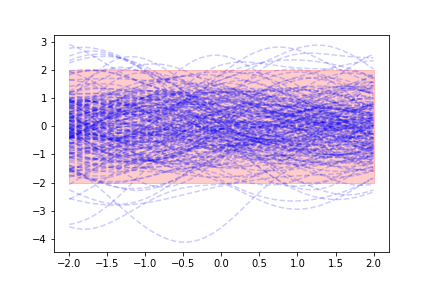
\includegraphics[width=0.45\textwidth]
		{figs/gprex1a.png}}
	\subfloat[GP posterior]{\label{gprex1b}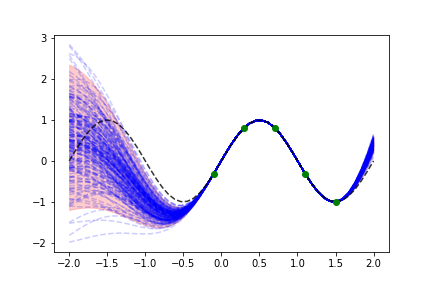
\includegraphics[width=0.45\textwidth]
		{figs/gprex1b.png}}
	
	\caption[Gaussian process regression of $f(x) = \sin(\pi x)$]{\label{gprfig}Gaussian process regression of $f(x) = \sin(\pi x)$. In (a), it is shown the prior space distribution, with samples path in blue and confidence interval in red. In (b), the posterior space distribution, after 4 measurements (in green) of $f(x)$ (black). Generating code can be found in \url{https://github.com/DFNaiff/Dissertation/blob/master/illustrations_dissertation/gp_prior_posterior}.}
\end{figure}


\subsection{Gaussian noise}
This equation can be generalized by assuming $p(y|x,M) = \mathcal{N}(y|f(x),\sigma^2_n)$. Then, letting $\epsilon \sim \mathcal{N}(0,\sigma^2_n)$, $\mathbf{y} = f(\mathbf{x})$, $\mathbf{y}^* = f(\mathbf{x}^*)$ and
\begin{equation} \label{jointGPnoise}
\left[ \begin{array}{c} 
\mathbf{y} \\
\mathbf{y}^* \end{array} \right] \sim \mathcal{N} 
\left( \left[ \begin{array}{c}
\mathbf{m}(\mathbf{x}) \\
\mathbf{m}(\mathbf{x}^*) \end{array} \right] , 
\left[ \begin{array}{c c} 
K(\mathbf{x},\mathbf{x}) + \sigma_n^2 I & K(\mathbf{x},\mathbf{x}^*) \\
K(\mathbf{x}^*,\mathbf{x}) & K(\mathbf{x}^*,\mathbf{x}^*) + \sigma^2_n I \end{array} \right]
\right).
\end{equation}
Conditioning $\mathbf{y}^*$ on $\mathbf{y}$ and, letting $K_\sigma(\mathbf{x},\mathbf{x}) := K(\mathbf{x},\mathbf{x}) + \sigma_n I$, we have
\begin{equation}\label{meancovGPR}
\begin{split}
& \mathbf{y}^* | \mathbf{x}^\star, \mathcal{D}, M = \mathbf{y}^*|\mathbf{y},M \sim \mathcal{N}(\mu^\star,\Sigma^*) \\
& \mu^\star = \mathbf{m}(\mathbf{x}^\star) + K(\mathbf{x}^\star,\mathbf{x}) K_\sigma(\mathbf{x},\mathbf{x}){-1} (\mathbf{y} - m(\mathbf{x})) \\
& \Sigma^\star = K(\mathbf{x}^\star,\mathbf{x}^\star) - K(\mathbf{x}^\star,\mathbf{x}) K_\sigma(\mathbf{x},\mathbf{x})^{-1} K(\mathbf{x}^\star,\mathbf{x}) + \sigma_n I.
\end{split}
\end{equation}
Notice \eqref{meancovGPR} reduces to \eqref{meancovGPRpure} when $\sigma^2_n = 0$. 
\subsection{General noise}
In the general case where $p(y|x,M)$ = $p(y|f(x))$, there is not a closed form solution and one must resort to explicit marginalization and Bayes' rule:
\begin{equation}\label{generalnoise}
\begin{split}
 & p(y_*|x_*,\mathcal{D}) = \\  & = 
  \int p(y_*|f(x_*)) p(f(x_*)|x_*,\mathbf{x},\mathbf{y}) df(x_*)\\ & = 
  \int p(y_*|f(x_*)) \int p(f(x_*)|x_*,f(\mathbf{x}), \mathbf{x}) p(f(\mathbf{x}) | \mathbf{x},\mathbf{y}) df(\mathbf{x}) df(x_*) \\ & \propto
  \int p(y_*|f(x_*)) \int p(f(x_*)|x_*,f(\mathbf{x}), \mathbf{x}) p(\mathbf{y}|f(\mathbf{x})) p(f(\mathbf{x})|\mathbf{x}) df(\mathbf{x})df(x_*).
 \end{split}
\end{equation}
Since $p(f(\mathbf{x})|\x) = \mathcal{N}(f(\mathbf{x})|m(\mathbf{x}),K(\mathbf{x},\mathbf{x}))$ and $p(f(x_*)|x_*,f(\mathbf{x}), \mathbf{x})$ is given by \eqref{meancovGPRpure}, these two terms may be joined together by \eqref{productgaussians}. However, this still leaves a double integral, that must be treated by approximate inference methods.

\subsection{Mean function}
Usually, the mean function $m$ is set to zero, letting the covariance function determine the whole structure of the regression. This is a reasonable assumption since, for any $f \sim GP(m,k)$, due to the sum of a Gaussian distribution and a constant being itself Gaussian with the constant added to its mean, we have $f-m \sim GP(0,k)$. Thus, fixed the model $(m,k)$, one can then do the GP regression on $f-m$ and then later add $m$. This is particularly useful if it is assumed that $f$ is modeled by some function $m$ that is known to be an incomplete model, thus complementing the regression by modeling this incompleteness by a zero mean GP.

\section{Covariance functions}

As said in the previous section, covariance functions $k$ must be PSD. This raises the question on which kind of functions are PSD, thus able to define a GP. A few functions can be easily shown to be PSD directly by their definitions, such as:
\begin{itemize}
	\item The constant function $k(x,x') = c \geq 0$, since the matrix $K_{i,j} = c$ is PSD, for all $c \geq 0$
	\item $k(x,x') = \mathbb{I}_{x = x'}$, since the corresponding matrix $K$ is the identity matrix
	\item If $\mathcal{X} = \{x_1,...,x_N\}$  is a finite set of size $N$, and $k$ is such that, for $\mathbf{x} = (x_1,...,x_N)$, 
	$K(\mathbf{x},\mathbf{x})$ is PSD, then $k$ is PSD, since for any other subset of $\mathcal{X}$, the corresponding kernel matrix will be a subset of $K$, thus also PSD \cite{hogben14}.
	\item If we have an explicit feature map $\Phi : \mathcal{X} \to \mathbb{R}^N$, then $k(x,x') = \langle \Phi(x),\Phi(x') \rangle$ is PSD \cite{Shawe_Taylor_2004}. For instance, if $\mathcal{X} = \mathbb{R}$ and $\Phi(x) = (x,x^2,\ldots,x^N)$, then $k(x,x') = \sum_{i=1}^N (x x')^i$ is PSD.
\end{itemize}
However, for many covariance functions, direct proof of being PSD is infeasible. However, there are some covariance functions that can be shown to be PSD in a indirect way, as shown below.
\subsubsection{Stationary covariance functions}
\begin{Definition}
	Let $\mathcal{X} = \mathbb{R}^d$. An covariance function is \textit{stationary} if $k(x,x') = k(x - x')$ , 
	for $k : \mathbb{R}^d \to \mathbb{R}$ \footnote{Here we overload the notation, letting the reader infer whether $k$ refers to a covariance function or an autocavariance function by the number of its arguments.}. Conversely, $k$ is a \textit{autocovariance function} if $k(x,x') = k(x - x')$ is a covariance function.
\end{Definition}
For this class of functions, we can reduce the analysis of $k$ to that of $k$. In particular, the next theorem says that one can analyze the Fourier transform of $k$ to check if it is an autocovariance function, thus $k$ being a covariance function (here, it is conveniente to consider $k$ as a function into $\mathbb{C}$).

\begin{Theorem}[Bochner's Theorem]
	A function $k : \mathbb{R}^d \to \mathbb{C}$, continuous at $0$, is an autocovariance function if and only if 
	\begin{equation}
	k(\tau) = \int_{\mathbb{R}^D} e^{2 \pi i \mathbf{s}^T \tau} d \mu (\mathbf{s}),
	\end{equation}
	where $\mu$ is a positive finite measure \cite{Stein_1999,Rasmussen06}.
	If $\mu$ has a density $S$, then $S$ an $k$ are Fourier duals of each other \cite{Chatfield_2004}.
	\begin{displaymath}
	\begin{split}
	k(\tau) & = \int_{\mathbb{R}^D} e^{2 \pi i \mathbf{s}^T \tau} S(\mathbf{s}) d\mathbf{s} \\
	S(\mathbf{s}) & = \int_{\mathbb{R}^D} e^{-2 \pi i \mathbf{s}^T \tau} k(\tau) d \tau.
	\end{split}
	\end{displaymath}
	In this case, $S$ is called the \text{spectral density} corresponding to $k$.
\end{Theorem}


One particular case of stationary functions are \textit{isotropic} functions, in which $k(\tau)$ is a function of $r = ||\tau||_2$. In this case, $S(\mathbf{s})$ is a function of $s = ||\mathbf{s}||_2$ \cite{CIS-4647}. For simplicity, those will also be referred as $k$ ans $S$. We show here some examples of isotropic covariance functions, along with their spectral densities (many others can be found in \cite{Rasmussen06}):
\begin{itemize}
	\item The squared exponential (SQE) kernel, also called RBF kernel 
	\begin{equation}\label{sqekernel}
	k_{SQE}(r;l) = \exp \left(-\frac{r^2}{l^2}\right),
	\end{equation}
	whose spectral density is given by a normal distribution
	\begin{equation}
	S(s;l) = (2 \pi l^2)^{D/2} \exp(-2 \pi^2 l^2 s^2)
	\end{equation}
	The squared exponential kernel is the most widely used in the field of Gaussian process, and kernel methods in general. However, the squared exponential kernel generates functions that are infinitely differentiable, thus being far too smooth for some applications. Moreover, the resulting kernel matrix tends to be very ill-conditioned, which results in numerical issues in applications with low noise.
	\item The \text{Matérn} class of kernels, parameterized by $\nu > 0$, given by
	\begin{equation}\label{maternkernel}
	k_{Matern,\nu}(r;l) = \frac{2^{1-\nu}}{\Gamma(\nu)} \left(\frac{\sqrt{2 \nu} r}{l} \right)^\nu
	K_\nu \left( \frac{\sqrt{2 \nu} r}{l} \right),
	\end{equation}
	where $K_\nu$ is the modified Bessel function of second kind. The corresponding spectral density 
	is a $2 \nu$-degreed multivariate t-distribution
	\begin{equation}
	S_\nu(s;l) = 2^D \pi^{D/2} \frac{\Gamma(\nu + D/2)(2 \nu)^\nu}{\Gamma(\nu)l^{2 \nu}}\left(\frac{2 \nu}{l^2} + 
	4 \pi^2 s^2\right)^{-(2 \nu+D)/2}.
	\end{equation}
	If $\nu$ is a half-integer, the kernel formula is simplified to a product of a polynomial of order $\nu - 1/2$ and an exponential. The most commonly used values of $\nu$ are:
	\begin{itemize}
		\item $\nu = 1/2$, giving $k_{Matern,1/2}(s;l) = \exp(-r/l)$.
		\item $\nu = 3/2$, giving $k_{Matern,3/2}(s;l) = \left(1 + \sqrt{3} r/l \right) \exp(-\sqrt{3}r/l)$.
		\item $\nu = 5/2$, giving $k_{Matern,5/2}(s;l) = \left(1 + \sqrt{5} r/l + 5 r^2/l^2 \right) \exp(-\sqrt{5}r/l)$.
	\end{itemize}
	In the limit $\nu \to \infty$, the Matern kernel converges to the squared exponential kernel \cite{Stein_1999}. In practice, for values of $\nu \geq 7/2$, the Matern kernel is similar enough to the squared exponential kernel to be of use, thus in practice only the three values of $\nu$ shown above are used.
	\item The spectral mixture kernel \cite{wilson2013gaussian}
	\begin{equation}\label{spectralmixturekernel}
	k_{SM}(\tau) = \sum_{q=1}^Q w_q \prod_{d=1}^D \exp(-2 \pi^2 \tau_d^2 v_{q}^{(d)})
	\cos(2 \pi \tau^{(d)} \mu_q^{(d)}),
	\end{equation}
	which is constructed explicitly as the Fourier dual of mixtures of multivariate normal densities. In \cite{wilson2013gaussian}, it is argued that the spectral mixture kernel approximates many of the kernels in \cite{Rasmussen06}, given enough mixtures $Q$.
\end{itemize}


\subsection{Derived kernels}
Although PSD functions are relatively hard to find, even with the use of Bochner's Theorem, one can prove that many compositions of base PSD functions are themselves PSD, thus providing many new classes of kernels.
Given $\mathcal{X}$ an arbitrary set, $k_1$,$k_2$ PSD functions on $\mathcal{X}$, and $k_3$ a PSD function on a set $\mathcal{Y}$, we have:
\begin{itemize}
	\item $k(x,x') := k_1(x,x') + k_2(x,x')$ is a PSD function, since, for $\mathbf{x} = (x_1,...,x_N) \in \mathcal{X}^N$, $K(\mathbf{x},\mathbf{x}) = K_1(\mathbf{x},\mathbf{x}) + K_2(\mathbf{x},\mathbf{x})$, the sum 
	of two PSD matrices, hence a PSD matrix. Similarly, $k(x,x') := k_1(x,x') k_2(x,x')$ is a PSD function, since $K(\mathbf{x},\mathbf{x}) = K_1(\mathbf{x},\mathbf{x}) \odot K_2(\mathbf{x},\mathbf{x})$ (where $A \odot B$ denotes the Hadamard product between $A$ and $B$), and, according to Schur product theorem \cite{hogben14}, $K(\mathbf{x},\mathbf{x})$ is also PSD as the Hadamard product of two PSD matrices.
	\item $k([x,y],[x',y']) = k_1(x,x') + k_3(y,y')$ is a PSD function, and so is $k([x,y],[x',y']) = k_1(x,x') k_3(y,y')$. This follows from the fact that both sum and Hadamard product of PSD matrices are PSD.
	\item For a map $f : \mathcal{Y} \to \mathcal{X}$, $k(y,y') = k_1(f(x),f(x'))$ is aPSD. This follows directly from the fact that if $y_i = f(x_i), \ i=1,...,n$, 
	$K(\mathbf{y},\mathbf{y}) = K_1(f(\mathbf{x}),f(\mathbf{x}'))$. This property allows us to construct non-stationary kernels from stationary kernels, by using input warping functions. Moreover, 
	this implies that we can substitute $r = ||\mathbf{x} - \mathbf{x}'||_2$ for $r = \sqrt{(\mathbf{x} - \mathbf{x})^T A^{-1} (\mathbf{x} - \mathbf{x})}$, where $A$ is a positive definite matrix, by setting $f(x) = A^{-1/2} x$
\end{itemize}
The last item allows us to construct kernels with general \textit{outputscale} and \textit{lengthscale} from stationary kernels. That is, if $k_0$ is an autocovariance function such that $k_0(0) = 1$, then
\begin{equation}\label{scaledkernels}
k(x-x') = \theta k\left(\frac{x_1-x'_1}{l_1},\ldots,\frac{x_D-x'_D}{l_D}\right) 
\end{equation}
is a kernel with outputscale $\theta$ and lengthscales $l_1,\ldots,l_D$. We call such kernels \textit{anisotropic} (although strictly speaking, every non-isotropic kernel is anisotropic).

\section{Model selection}
In the above discussion, the model $M = (m,k)$ was assumed to be fixed. In practice, since we have many different kernel functions, each parameterized by a continuous set of parameters (called \textit{hyperparameters}), we need a way to choose the correct model. In the noisy measurement case, we also need to deal with the noise distribution parameters. Fortunately, the Bayesian framework gives a natural way to choose the model. 

Assume $p(y|f(x)) = \mathcal{N}(f(x),\sigma_n^2)$. Then, 
\begin{displaymath}
\mathcal{D}|M,\sigma_n = \mathbf{y} | \mathbf{x},M,\sigma_n \sim 
\mathcal{N}(m(\mathbf{x}),K(\mathbf{x},\mathbf{x}) + \sigma_n \mathbf{I}).
\end{displaymath}
Therefore, the likelihood for the model is given by 
\begin{equation}\label{loglikelihoodGP}
\begin{split}
\log p(\mathcal{D}|M,\sigma_n) = & -\frac{1}{2}(\mathbf{y} - m(\mathbf{x}))^T (K(\mathbf{x},\mathbf{x}) + \sigma_n \mathbf{I})^{-1} (\mathbf{y} - m(\mathbf{x})) + \\
&-\frac{1}{2} \log \det (K(\mathbf{x},\mathbf{x}) + \sigma_n \mathbf{I}) - \frac{1}{2} N \log(2\pi).
\end{split}
\end{equation}
The important thing to notice is that the likelihood above is actually a marginal likelihood, since
\begin{equation}
p(\mathcal{D}|M,\sigma_n) = \Ev_{f \sim GP(m,k)} \left[p(\mathcal{D}|f,\sigma_n) \right].
\end{equation}
Hence, it should display the Occam's razor effect. In fact, the log-determinant term does exactly this, acting as a sort of regularizer. However, this does not mean that GP regression is protected from overfitting (see \cite{Mohammed_2017}). Moreover, since the objective function is non-convex, there may be local optima that returns spurious results.

A fully Bayesian approach to GP regression is desirable in order to incorporate fully the hyperparameter knowledge. However, when the number of data is considerably large, Monte Carlo methods becomes inefficient (although it can be used still, see for example \cite{Neal_1997,Petelin_2014}). In \cite{Osborne_2007}, an approach based on Bayesian Monte Carlo (to be presented in Chapter 4) is also explored. However, efficient marginalization of hyperparameters remains an open problem.

\section{Computational issues}
\subsection{Jittering}
If the noise $\sigma_n^2$ is zero, the matrix $K(\mathbf{x},\mathbf{x})$ may be ill-conditioned, which is usually the case for the SQE kernel. One way to mitigate this problem is to force the existence of an "artificial noise" on $K(\mathbf{x},\mathbf{x})$, that is, one substitute it for $K(\mathbf{x},\mathbf{x}) + \sigma^2_j I$, where $\sigma^2_j$ is not a real noise parameter now, but just an stabilizer. In this case, the error caused by the addition of artificial noise is considerably smaller than the error of numerical operations in ill-conditioned matrices, if they are able to be performed at all. The Cholesky decomposition (described below) also helps with the stability of inverse matrix operations.

\subsection{Scaling with data}\label{scalinggpsession}
The main issue with GP regression is that, given $N$ training points, for a fixed covariance function the evaluations in \eqref{meancovGPR} requires at least one operation with the inverse of a $N \times N$ matrix $K(\mathbf{x},\mathbf{x} + \sigma_n \mathbf{I})$, whose computational cost is of order $\mathcal{O}(N^3)$. The problem is worsened in the case of training a model, since this operation has to be done for each evaluation of $\log p(\mathcal{D}|M,\sigma_n,\theta)$ while training. 

Since $K(\mathbf{x},\mathbf{x}) + \sigma_n \mathbf{I}$ is a positive definite matrix, one can try to mitigate the computational cost by computing the Cholesky decomposition
\begin{displaymath}
K(\mathbf{x},\mathbf{x}) + \sigma_n \mathbf{I} = L L^T.
\end{displaymath}
Then, given the decomposition, the inverse operations involve inverses of triangular matrices, whose operations costs are of order $\mathcal{O}(N^2)$, while the determinant term in $\log p(\mathcal{D}|M,\sigma_n,\theta)$ can be calculated as $\log \det (L L^T) = 2 \sum_i \log L_{ii}$. However, Cholesky decomposition, although faster than other methods like the LU decomposition, still has a computational cost of $\mathcal{O}(N^3)$, hence the scaling problem still exists.

\section{Online learning}\label{onlinelearningsection}
One interesting aspect of GPs is its ability to accumulate online data in a relatively simple manner, provided we do not change its hyperparameters. Consider fixed an initial data $\mathcal{D} = \{(x_i,y_i)\}_{i=1}^N$, and a GP model $(m,k)$, if we have a kernel matrix $K_{\mathcal{D}}$, and its Cholesky factor $L_{\mathcal{D}}$, resulting in a readily accessible posterior mean function $m_\mathcal{D}(x)$ and covariance function $k_\mathcal{D}(x,x')$. Now, suppose some new data $\mathcal{D}' = \{(x'_j,y'_j)\}_{j=1}^M$ is available, and the practitioner wants to incorporate into a new posterior mean $m_{\mathcal{D} \cup \mathcal{D}'}(x,x')$ and covariance $k_{\mathcal{D} \cup \mathcal{D}'}(x,x')$. A naive manner for doing this would be constructing a new kernel matrix $K_{\mathcal{D} \cup \mathcal{D}'}$ from scratch, and compute its Cholesky factor $L_{\mathcal{D} \cup \mathcal{D}'}$, resulting in a operation cost $\mathcal{O}((M + N)^3)$. Fortunately, there is a clever way to obtain $L_{\mathcal{D} \cup \mathcal{D}'}$ from $L_\mathcal{D}$ with $\mathcal{O}(M^3 + MN^2)$ cost (assuming $K_{\mathcal{D} \cup \mathcal{D}'}$ stays positive-definite). The following argument is adapted from \cite{Osborne_2012}, where it is considered the upper Cholesky factor.

To see this, consider $\mathbf{x}_N = (x_i)_{i=1}^N$, $\mathbf{x}_M = (x'_j)_{j=1}^M$ and $\mathbf{x} = \mathbf{x}_N \cup \mathbf{x}_M$ (here $\cup$ denotes concatenation). Then, noting $K_\mathcal{D} = K(\x_N,\x_N)$, we have 
\begin{equation}
 K_{\mathcal{D}\cup\mathcal{D}'} = \left[ \begin{array}{cc}
K(\x_N,\x_N) & K(\x_N,\x_M) \\
K(\x_M,\x_N) & K(\x_M,\x_M) \end{array} \right].
\end{equation}
Then $L_{\mathcal{D}\cup\mathcal{D}'}$ must be of the form
\begin{equation}\label{formatcholexpanded}
L_{\mathcal{D}\cup\mathcal{D}'} = \left[ \begin{array}{cc}
L_\mathcal{D} & 0 \\
S & \tilde{L} \end{array} \right],
\end{equation}
with $\tilde{L}$ being lower triangular. This is because
\begin{equation}
\begin{split}
L_{\mathcal{D}\cup\mathcal{D}'} L_{\mathcal{D}\cup\mathcal{D}'}^T = \left[ \begin{array}{cc}
L_\mathcal{D} & 0 \\
S & \tilde{L} \end{array} \right] \left[ \begin{array}{cc}
L_\mathcal{D}^T & S^T \\
0 & \tilde{L}^T \end{array} \right] & = \left[ \begin{array}{cc}
L_\mathcal{D} L_\mathcal{D}^T & L_\mathcal{D} S^T \\
S L_\mathcal{D}^T & S S^T + \tilde{L} \tilde{L}^T \end{array} \right] \\
 & = \left[ \begin{array}{cc}
K(\x_N,\x_N) & K(\x_N,\x_M) \\
K(\x_M,\x_N) & K(\x_M,\x_M) \end{array} \right] = K_{\mathcal{D}\cup\mathcal{D}'}.
\end{split}
\end{equation}
This readily shows not only that $L_{\mathcal{D}\cup\mathcal{D}'}$ must be of the format in \eqref{formatcholexpanded}, but it gives a way to get $S$ and $\tilde{L}$: calculate $S= \big( L_\mathcal{D}^{-1} K(\x_N,\x_M) \big)^T$, and $\tilde{L}$ is the lower Cholesky factor of $K(\x_M,\x_M) - SS^T$, whose operations are of cost $\mathcal{O}(N^2 M)$ and $\mathcal{O}(M^3)$.          % Editar o arquivo capituloB.tex
\chapter{Bayesian Monte Carlo}
Consider the integral
\begin{equation}\label{integralbmc}
Z = \int_{\mathbb{R}^D} f(x) p(x) dx.
\end{equation}
In the following discussion, we drop  $\mathbb{R}^D$ from the integral symbol, for simplicity. If $p(x)$ is a distribution whose sampling is easy, the bottleneck for a simple Monte Carlo method for estimating $Z$ would be the evaluation cost of $f$. If evaluating $f$ is costly then, a naive Monte Carlo method often becomes infeasible. In this section, we present a GP-based method that tries to circumvent this bottleneck. 

\section{GP approximation for the integrand}
In Bayesian Monte Carlo (BMC), or Bayesian quadrature \cite{Ghahramani_2003,O_Hagan_1991} \footnote{The original name Bayesian quadrature describes more accurately the method, however the name Bayesian Monte Carlo will be used in this text. At the literature, both names can be found in roughly equal proportion}, $f$ itself is treated as a random function, and a GP prior $GP(m,k)$ is put on $f$. Therefore, given a set $\mathcal{D} = \{(x_i,f(x_i))\}_{i=1}^N$ of $N$ evaluations, the posterior random function $f_{\mathcal{D}}$ is also distributed according to a GP. In particular, since linear maps of GPs are themselves GPs \cite{Rasmussen06,Hennig_2012}, this implies that the random variable
\begin{equation}\label{bmcrv}
Z_{\mathcal{D}} = \int f_{\mathcal{D}}(x) p(x) dx
\end{equation}
is a Gaussian random variable. Since we can find the mean by 
\begin{equation}\label{evbmc}
\begin{split}
\Ev[Z_{\mathcal{D}}] = \Ev \left[\int f_{\mathcal{D}}(x) p(x) dx \right] = \int \Ev[f_{\mathcal{D}}(x)] p(x) dx,
\end{split}
\end{equation}
and the variance by,
\begin{equation}\label{varbmc}
\begin{split}
\Var(Z_{\mathcal{D}}) & = \Ev[(Z_{\mathcal{D}} - \Ev[Z_{\mathcal{D}}])^2] \\
& = \Ev \left[\left( \int (f_{\mathcal{D}}(x) - \Ev[f_{\mathcal{D}}(x)]) p(x) dx \right)^2 \right] \\
& = \int \int \Ev \left[(f_{\mathcal{D}}(x) - \Ev[f_{\mathcal{D}}(x)]) (f_{\mathcal{D}}(x') - \Ev[f_{\mathcal{D}}(x')]) \right]  p(x) p(x') dx dx' \\
& = \int \int \Cov(f_{\mathcal{D}}(x),f_{\mathcal{D}}(x')) p(x) p(x') dx dx'.
\end{split}
\end{equation}
We have a complete description of the distribution of $Z_\mathcal{D}$. Now, by substituting \eqref{meancovGPR} in \eqref{evbmc} and \eqref{varbmc}, we have 
\begin{equation}\label{evvarbmc2}
\begin{split}
& \Ev[Z_{\mathcal{D}}] = \int m(x) p(x) dx - \mathbf{z}^T K^{-1} (\mathbf{f}-m(\mathbf{x})) \\
& \Var[Z_{\mathcal{D}}] = \Gamma - \mathbf{z}^T K^{-1} \mathbf{z},
\end{split}
\end{equation}
where $\mathbf{z} = (z_1,...,z_N)^T$, with
\begin{equation}\label{zbmcdef}
z_i = \int k(x,x_i) p(x) dx,
\end{equation}
and 
\begin{equation}\label{varcoef}
\Gamma = \int \int k(x,x') p(x) p(x') dx dx'.
\end{equation}
In general, a good estimate of $Z_\mathcal{D}$ is its mean, although if there is an asymmetric loss function associated with estimating $Z_\mathcal{D}$, its variance should be taken in account.

An illustration of the Bayesian Monte Carlo approach to integration is shown in Figure \ref{bmcfig}. There, the distribution is $p(x) = \mathcal{N}(x|0,0.5)$, and $f(x) = -x^2$. The true value of the integral, and BMC estimation are shown. Notice that, in this example, for $|x|>2$ the GP estimate $m_\mathcal{D}(x)$ of $f(x)$ becomes very inaccurate. However, since low probability mass is assigned outside the interval, the BMC estimation is still close to the target.

\begin{figure}
	\centering
	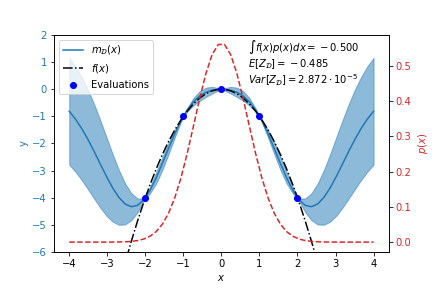
\includegraphics[width=0.7\linewidth]{figs/exbmc.png}
	\caption[Illustration of Bayesian Monte Carlo integration]{\label{bmcfig} Illustration of Bayesian Monte Carlo integration. Here, dash-dot black is $f(x)$, whose value is on the left-axis, while in blue is it's GP mean (dark), and covariance (light), given 5 evaluations (blue circles). In red is $p(x)$, whose value is on the right axis. The true value of the integral, the BMC mean and variance are shown on the top right.}
\end{figure}

\subsection{Philosophical remark}
At first one may find strange to consider $f$ as a random function, in order to give a prior for it. After all, $f$ is a known, fixed function. However, notice that $f$ is only actually known in so far as one can evaluate it, and if evaluations for $f$ are limited, so is the knowledge of it. And by the discussion in Chapter 1, any object the learner has limited knowledge about should be considered a random variable, independent of the fact that the object is actually random or not.

If this philosophical approach is not convincing, maybe it is better to just think of the BMC method as an artificial way to integrate functions, and follow the famous dictum in quantum mechanics: "Shut up and calculate" \cite{Mermin_2004}.


\section{Kernel-distribution combinations}\label{kerneldistributionbmc}
In general, neither \eqref{zbmcdef} nor \eqref{varcoef} are analytically available, just like the original integral \eqref{integralbmc}. However, evaluating the kernel function is in general cheap, so if evaluation of $f$ is expensive, there may be still computational gains in using BMC. For some particular distributions $p(x)$, combined with some suitable kernel choices, \eqref{zbmcdef} nor \eqref{varcoef} does lend analytical solutions, or can be treated in a relatively cheap manner. In the following, $m(x) = 0$ for simplicity, thus omitting the term.

\subsection{SQE kernel with Gaussian distributions}
Assume $p(x) = \mathcal{N}(x|\mu,\Sigma)$, and $k$ is a anisotropic squared exponential kernel, with vertical scale $\theta$ and length scales $l = (l_1,...,l_D)$. Notice then that, by letting $A := \text{diag}(l_1^2,...,l_D^2)$, we have 
\begin{equation} \label{rbfasnormal}
\begin{split}
k(x,x') = \theta \exp \left( -\frac{1}{2} (x - x')^T A^{-1} (x - x') \right) = & \det(2 \pi A) \mathcal{N}(x'|x,A) = \\
& \det(2 \pi A) \mathcal{N}(x|x',A).
\end{split}
\end{equation}
Then, by \eqref{productgaussians}:
\begin{equation} \label{kpexpansion1}
\begin{split}
& k(x,x') \mathcal{N}(x|\mu,\Sigma) = C(x') \mathcal{N}(x|\tilde{\mu}_{x'},\tilde{\Sigma}) \\
& C(x') = \frac{\theta}{\det(I + A^{-1} \Sigma)^{1/2}} \exp \left(-\frac{1}{2}(x' - \mu)^T (A + \Sigma)^{-1}(x' - \mu) \right) \\
& \tilde{\mu}_{x'} = (A^{-1} + \Sigma^{-1})^{-1} (A^{-1} x' + \Sigma^{-1} \mu) \\
& \tilde{\Sigma} = (A^{-1} + \Sigma^{-1})^{-1},
\end{split}
\end{equation}
and
\begin{equation} \label{kpexpansion2}
\begin{split}
& k(x,x') \mathcal{N}(x|\mu,\Sigma) \mathcal{N}(x'|\mu,\Sigma) = \hat{C} \mathcal{N}(x|\tilde{\mu}_{x'},\tilde{\Sigma}) \mathcal{N}(x'|\tilde{\mu}_{x},\tilde{\Sigma}) \\
& \hat{C} = \frac{\theta}{\det(I + 2 A^{-1} \Sigma)^{1/2}}.
\end{split}
\end{equation}
Hence, by substituting \eqref{kpexpansion1} and \eqref{kpexpansion2} into \eqref{zbmcdef} and \eqref{varcoef}, we find 
\begin{equation}\label{termsbmcgaussian}
\begin{split}
& z_i = \frac{\theta}{\det(I + A^{-1} \Sigma)^{1/2}} \exp \left(-\frac{1}{2}(x_i - \mu)^T (A + \Sigma)^{-1}(x_i' - \mu) \right) \\
& \Gamma = \frac{\theta}{\det(I + 2 A^{-1} \Sigma)^{1/2}}.
\end{split}
\end{equation}
Substituting in \eqref{evvarbmc2} we find the desired result:
\begin{equation}\label{evvarbmcgaussian}
\begin{split}
& \Ev[Z_{\mathcal{D}}] = \mathbf{z}^T K^{-1} \mathbf{f} \\
& \Var[Z_{\mathcal{D}}] = \frac{\theta}{\det(I + 2 A^{-1} \Sigma)^{1/2}} - \mathbf{z}^T K^{-1} \mathbf{z} \\
& z_i = \frac{\theta}{\det(I + A^{-1} \Sigma)^{1/2}} \exp \left(-\frac{1}{2}(x_i - \mu)^T (A + \Sigma)^{-1}(x_i' - \mu) \right) \\
& \Gamma = \frac{\theta}{\det(I + 2 A^{-1} \Sigma)^{1/2}}.
\end{split}
\end{equation}

\subsection{Mixture distributions}\label{bmcmixtures}
Consider taking expectations in respect to a mixture distribution
\begin{equation}
 p(x) = \sum_{i=1}^M \alpha_i p_i(x).
\end{equation}
From \eqref{zbmcdef} and \eqref{varcoef}, it is straightforward to see that in this case
\begin{equation}
\begin{split}
 z_i & = \sum_{i=1}^M \alpha_i \int k(x,x_i) p_i(x) dx \\
 \Gamma &= \sum_{i=1}^M \sum_{j=1}^M \alpha_i \alpha_j \int \int k(x,x') p_i(x) p_j(x') dx dx'.
\end{split}
\end{equation}
Then, provided it is possible to calculate the integrals above for each component $p_i(x)$, one can easily use mixture distributions from these coefficients.


An important case is considering mixtures of normal distributions $p(x) = \sum_{j=1}^{M} \alpha_j \mathcal{N}(x|\mu_j,\Sigma_j)$, and the squared-exponential kernel. Then, by substituting in \eqref{zbmcdef} and \eqref{varcoef}, and considering the results for normal distributions in \eqref{termsbmcgaussian}, we find 
\begin{equation}\label{bmcmixgaussians}
\begin{split}
 & z_i = \sum_{j=1}^M \alpha_j z_{i,j} \\ 
 & z_{i,j} = \frac{\theta}{\det(I + A^{-1} \Sigma_j)^{1/2}} \exp \left(-\frac{1}{2}(x_i - \mu_j)^T (A + \Sigma_j)^{-1}(x_i' - \mu_j) \right) \\
 & \Gamma = \sum_{j=1}^M \sum_{m=1}^M \alpha_j \alpha_m \Gamma_{j,m}, \\
 & \Gamma_{j,m} = \frac{\theta}{\det(I + A^{-1} (\Sigma_j+\Sigma_m))^{1/2}} \exp \left(-\frac{1}{2}(\mu_j-\mu_m)^T (A + \Sigma_j + \Sigma_m)^{-1}(\mu_j-\mu_m)\right).
\end{split}
\end{equation}

\subsection{Tensor product kernels and diagonal-covariance Gaussian distributions}\label{tensorprodbmc}
Consider tensor product kernels in $\mathbb{R}^D$ of the form
\begin{equation}
 k(x,x') = \prod_{d=1}^D k_d(x_d,x'_d),
\end{equation}
and a Gaussian distribution $p(x) = \mathcal{N}(x|\mu,\Sigma)$ with diagonal covariance $\Sigma = \text{diag}(\sigma_1^2,\ldots,\sigma_D^{d})$, so that $p(x) = \prod_{d=1}^D \mathcal{N}(x_d|\mu_d,\sigma_d^2)$. Then, 
\begin{equation}\label{prodkernelz}
\begin{split}
 z_i & = \int \prod_{d=1}^D k_d(x_d,x_{i,d}) \prod_{d=1}^D \mathcal{N}(x_d|\mu_d,\sigma_d^2) dx \\
 & = \prod_{d=1}^D \int k_d(x,x_{i,d}) \mathcal{N}(x|\mu_d,\sigma_d^2) dx,
\end{split}
\end{equation}
and 
\begin{equation}\label{prodkernelgamma}
\begin{split}
 \Gamma & = \int \int \prod_{d=1}^D k_d(x_d,x'_d) \prod_{d=1}^D \mathcal{N}(x_d|\mu_d,\sigma_d^2) \prod_{d=1}^D \mathcal{N}(x'_d|\mu_d,\sigma_d^2) dx dx' = \\
 & = \prod_{d=1}^D \int \int k_d(x,x')\mathcal{N}(x|\mu_d,\sigma_d^2)\mathcal{N}(x'|\mu_d,\sigma_d^2) dx dx'.
\end{split}
\end{equation}
Consider each individual component in \eqref{prodkernelz}. Even with none of then being analytically computable, they can easily be approximated using Gauss-Hermite quadrature, that approximates 
\begin{equation}\label{gausshermite}
\int f(x) \mathcal{N}(x|\mu,\sigma^2) dx \approx \frac{1}{\sqrt{\pi}} \sum_{k=1}^K w_k f(\sqrt{2} \sigma x_k + \mu),
\end{equation}
where $x_i$ are the roots of the physicists' Hermite polynomial
\begin{equation}
 H_K(x) = (-1)^N e^{x^2} \frac{d^K}{dx^K} e^{-x^2},
\end{equation}
and $w_k$ are the associated weights
\begin{equation}
 w_k = \frac{2^{K-1} K! \sqrt{\pi}}{K^2 (H_{K-1}(x_k))^2}.
\end{equation}
An analysis of this approximation can be found in \cite{Liu_1994}. It is important to notice that for each $K$, $\{(x_k,w_k)\}_{k=1}^K$ are fixed, unlike standard Monte Carlo methods that would require sampling from $\mathcal{N}(x|\mu,\sigma^2)$. Applying \eqref{gausshermite} to \eqref{prodkernelz}, one finds that
\begin{equation}
 z_i \approx \prod_{d=1}^D \frac{1}{\sqrt{\pi}}\sum_{k=1}^K w_k k_d(\sqrt{2} \sigma_d x_k + \mu_d,x_{i,d}),
\end{equation}
and that
\begin{equation}
\Gamma \approx \prod_{d=1}^D \frac{1}{\pi} \sum_{k,k'=1}^K w_k w_{k'} k_d(\sqrt{2} \sigma_d x_k + \mu_d,\sqrt{2} \sigma_d x_{k'} + \mu_d).
\end{equation}

By the discussion in section \ref{bmcmixtures}, one can easily extend this to mixtures of Gaussians with diagonal covariance. Therefore, one is free to use more flexible kernels than the squared exponential one, provided they are tensor product kernels. The trade-off is that $p(x)$ is a more restrictive distribution, but, as discussed next, this is not an insurmountable restriction. Moreover, the techniques presented in chapters 4 and 5 uses exactly those kinds of distributions as approximations.

\subsection{Importance reweighting for Bayesian Monte Carlo}
One can use the above results for doing integral estimations for general distributions using squared exponential kernels, without Monte Carlo integration of kernels, by an importance re-weighting trick
\begin{equation}
\int f(x) p(x) dx = \int \frac{f(x) p(x)}{q(x)} q(x) dx,
\end{equation}
where $q(x)$ may be either a normal distribution or a mixture of normals. This becomes interesting because since mixtures of normals can approximate continuous densities arbitrarily close as the number of mixtures goes to infinity \cite{Epanechnikov_1969}, thus providing good re-weighting distributions.


\section{Bayesian Monte Carlo for positive integrands}\label{positivebmc}
For many cases the integral we are interested is one arising from marginalization:
\begin{equation}
 p(\mathcal{D}) = \int L(x) p(x) dx = \int p(\mathcal{D}|x) p(x) dx.
\end{equation}
In particular, in this case $L(x)$ must be a positive function. However, applying the BMC method naively can result in rather inaccurate evaluations, due to the fact that in general, GP regression can predict negative means even when all function evaluations are positive. This way, the positivity of the GP mean for $L(x)$ is not guaranteed, resulting in possibly pathological predictions \cite{Ghahramani_2003}.

In \cite{Osborne_2012}, it is proposed to make a GP regression by putting an prior over $\log L(x) \sim GP(m,k)$. However, this means that for predictive distribution in the original space, $L(x|x_{D}) \sim \text{Lognormal}(m_\mathcal{D}(x),k_\mathcal{D}(x,x))$, which results in
\begin{equation}\label{lntranswrong}
 \Ev \left[ \int L(x|x_\mathcal{D}) p(x) dx \right] = 
 \int e^{m_\mathcal{D}(x)+\frac{1}{2}k_\mathcal{D}(x,x)} p(x) dx,
\end{equation}
which is still non-tractable integral, requiring further approximations. It is proposed in \cite{OHagan_1992} a somehow complicated heuristic to circumvent this problem, relying in a number of approximations whose accuracy is questionable, and an inner application of BMC.

In \cite{Gunter_2014}, the transformation used is the square-root transformation, so the prior for GP regression is over $\tilde{L}(x) = \sqrt{2 L(x) - \alpha}$, with $\alpha$ being a small positive scalar, resulting in $L(x|x_\mathcal{D}) = \alpha + \frac{1}{2} \tilde{L}(x|x_\mathcal{D})^2$. However, this way we have $\Ev[L(x|x_\mathcal{D})] = \alpha + \frac{k_\mathcal{D}(x,x)}{2}(1+m_\mathcal{D}(x)^2)$, hence, just like \eqref{lntranswrong}, we can't arrive at a tractable mean. In order to circunvent this, in \cite{Gunter_2014} two approaches are proposed. The first is a linearization of $\alpha + \frac{1}{2} \tilde{L}(x|x_\mathcal{D})^2$ around $m_\mathcal{D}(x)$, resulting in 
\begin{equation}
 L(x|x_\mathcal{D}) \approx L^{\mathcal{L}}(x|x_\mathcal{D}) = \alpha - \frac{1}{2} m_\mathcal{D}(x)^2 + m_\mathcal{D}(x) \tilde{L}(x),
\end{equation}
which, since it is a affine transformation of $\tilde{L}(x)$, results an approximate GP distribution for $L(\cdot|x_\mathcal{D})$:
\begin{equation}\label{sqlinearization}
\begin{split}
 & L^{\mathcal{L}}(\cdot|x_\mathcal{D}) \sim GP(m_\mathcal{D}^\mathcal{L}(x),k_\mathcal{D}^\mathcal{L}(x)) \\
 & m_\mathcal{D}^\mathcal{L}(x) = \alpha + \frac{1}{2} m_\mathcal{D}(x) \\
 & k_\mathcal{D}^\mathcal{L}(x,x') = m_\mathcal{D}(x) k_\mathcal{D}(x,x') m_\mathcal{D}(x).
\end{split}
\end{equation}
The second proposal is to approximate $L(\cdot|x_\mathcal{D})$ by a random GP-distributed function $L^\mathcal{M}(\cdot|x_\mathcal{D}) = GP(m^\mathcal{M}_\mathcal{D},k^\mathcal{M}_\mathcal{D})$, where $m^\mathcal{M}_\mathcal{D}(x)$ and $k^\mathcal{M}_\mathcal{D}(x)$ are chosen so that $L^\mathcal{M}(\cdot|x_\mathcal{D})$ is moment-matched with $L(\cdot|x_\mathcal{D})$, that is,
 $m^\mathcal{M}_\mathcal{D}(x) = \Ev[L(x|x_\mathcal{D})]$ and $k^\mathcal{M}_\mathcal{D}(x,x') = \Cov(L(x|x_\mathcal{D}),L(x'|x_\mathcal{D}))$. This results in the approximation
 \begin{equation}\label{sqmomentmatched}
  \begin{split}
  & L^{\mathcal{M}}(\cdot|x_\mathcal{D}) \sim GP(m_\mathcal{D}^\mathcal{M}(x),k_\mathcal{D}^\mathcal{M}(x)) \\
  & m_\mathcal{D}^\mathcal{M}(x) = \alpha + \frac{1}{2} (m_\mathcal{D}(x) + k_\mathcal{D}(x,x)) \\
  & k_\mathcal{D}^\mathcal{M}(x,x') = \frac{1}{2} k_\mathcal{D}(x,x')^2 + m_\mathcal{D}(x) k_\mathcal{D}(x,x') m_\mathcal{D}(x).
  \end{split}
 \end{equation}
In particular, both approaches results in tractable integrals for gaussian distributions and SQE kernels.

The idea of moment-matching is extended to a general setting in \cite{Chai_2019}, where it is considered the integral \eqref{integralbmc}, where $f$ is now a function from $\mathbb{R}^D$ to a strict subset $\mathcal{Y}$ of $\mathbb{R}$. In the case presented previously, $\mathcal{Y} = (0,\infty)$, while another important case is $\mathcal{Y} = (0,1)$. Considering an bijective map $\epsilon : \mathbb{R} \to \mathcal{Y}$, it is placed a GP prior $GP(m,k)$ over $g = \epsilon^{-1} \circ f$. Then, the posterior distribution for $f(\cdot|x_\mathcal{D}$ is approximated by a moment-matched GP with mean
$m^\mathcal{M}_\mathcal{D}(x) = \Ev[\epsilon(g(x|x_\mathcal{D}))]$ and $k^\mathcal{M}_\mathcal{D}(x,x') = 
\Cov(\epsilon(g(x|x_\mathcal{D})),\epsilon(g(x'|x_\mathcal{D})))$. In particular, for $\epsilon^{-1}(x) = \log(x)$, the same warping considered in \cite{Osborne_2012}, the moment matched mean and covariance becomes 
\begin{equation}\label{logmomentmatched}
\begin{split}
 & m^\mathcal{M}_\mathcal{D}(x) = e^{m_\mathcal{D}(x) + \frac{1}{2}k_\mathcal{D}(x,x)}\\
 & k^\mathcal{M}_\mathcal{D}(x,x') =e^{m_\mathcal{D}(x) + \frac{1}{2}k_\mathcal{D}(x,x)} e^{m_\mathcal{D}(x') + \frac{1}{2}k_\mathcal{D}(x',x')} \left(e^{k_\mathcal{D}(x,x')}-1\right).
\end{split}
\end{equation}

However, when integrated this GP does not result in a integrable mean or variance. One further proposal of \cite{Chai_2019} is to do a Taylor expansion of $m^\mathcal{M}_\mathcal{D}(x)$, 
\begin{equation}\label{taylormomentmatched}
 m^\mathcal{M}_\mathcal{D}(x) \approx 1 + m_\mathcal{D}(x) + \frac{1}{2} k_\mathcal{D}(x,x) + \frac{1}{2}\left(m_\mathcal{D}(x) + \frac{1}{2} k_\mathcal{D}(x,x)\right)^2 + \ldots,
\end{equation}
and of $k^\mathcal{M}_\mathcal{D}(x,x')$,
\begin{equation}
\begin{split}
 k^\mathcal{M}_\mathcal{D}(x,x')  \approx 1 & + k_\mathcal{D}(x,x') + \frac{1}{2} k_\mathcal{D}(x,x')^2 \\ & +
 k_\mathcal{D}(x,x') \left(m_\mathcal{D}(x) + \frac{1}{2} k_\mathcal{D}(x,x) + m_\mathcal{D}(x') + \frac{1}{2} k_\mathcal{D}(x',x')\right)^2 + \ldots\end{split},
\end{equation}
which, depending on the mean function and kernel function (for instance, zero mean and SQE kernel), is integrable when truncated \cite{Chai_2019}.

The use of function warping raises a question on how to choose the GP hyperparameters. In \cite{Chai_2019}, it is argued that for the moment-matched procedure, one should choose the hyperparameters considering the approximated GP distribution for $f$,  $GP(m^\mathcal{M},k^\mathcal{M}(x,x'))$ and the data $(\mathbf{x},f(\mathbf{x}))$, as opposed to the exact GP distribution for $g$, where it is considered $GP(m,k)$ and the data $(\mathbf{x},g(\mathbf{x}))$. The authors of \cite{Chai_2019} call the first approach \textit{$f$-space} optimization, and the second one \textit{$g$-space} optimization, and it is argued that empirically, $f$-space optimization results in better integral estimations for their test cases. \footnote{Tests with $f$-space optimization in this work weren't successful.}

\section{Choosing evaluation points}

The integral estimate variance $\Var[Z_{\mathcal{D}}]$ yields a natural metric for choosing a set of evaluation points $X_\mathcal{D} = \{x_1,...,x_N\}$. Namely, since $\Var[Z_\mathcal{D}]$ does not depend on the evaluation values $\{f(x_1),\ldots,f(x_N)\}$, one can, given a budget of $N$ evaluations, minimize the function $\alpha_{\text{OBQ}}:\mathbb{R}^{dN} \to \mathbb{R}$ given by
\begin{equation}\label{optimal_bmc}
\alpha_{\text{OBQ}}(X_\mathcal{D}) =  \Var[Z_{\mathcal{D}}](X_\mathcal{D}) = \Gamma(X_\mathcal{D}) - \mathbf{z}(X_\mathcal{D})^T K(X_\mathcal{D})^{-1} \mathbf{z}(X_\mathcal{D})
\end{equation}
However, the evaluation of this function has a $\mathcal{O}(N^3)$ cost, due to the need for matrix inversion, is not necessarily convex, and is defined on a very high dimensional space, so its minimization will be feasible only in specific cases. An easier way would be to take a greedy approach, that is, given $X_{\mathcal{D}_{m}} = \{x_1,...,x_m\}$ previously chosen evaluation points, with $m < n$, we choose $x_{m+1}$ such that the variance of $Z_{\mathcal{D}_m \cup \{x_{m+1},f(x_{m+1})\}}$ is minimized, that is, we are looking to minimize the objective function 
\begin{equation}
\alpha^m_{\text{SBQ}}(x_{m+1}) = \alpha^m_\text{OBQ}(x_{m+1};x_1,\ldots,x_m)
\end{equation}

\begin{equation}\label{sequential_bmc}
\alpha^m_{SBQ} : \mathbb{R}^d \to \mathbb{R} , \quad x_{m+1} \to \Var[Z_{\mathcal{D}^m \cup \{x_{m+1},f(x_{m+1})\}}](x_{m+1}),
\end{equation}
This algorithm is referred as Sequential Bayesian Quadrature (SBQ) in \cite{Briol_2015}, while in the same work the first objective is referred as Optimal Bayesian Quadrature (OBQ). Notice that the kernel matrix Cholesky decomposition can be updated in $\mathcal{O}(N^2)$ by the discussion in Section \ref{onlinelearningsection}, and that this operation is differentiable, since the Cholesky decomposition is differentiable \cite{Smith_1995,Murray_2016}. 

One can simplify this objective function, by substituting it for an heuristic of finding the point of maximum variance of the integrand, that is, substituting
\begin{equation}
\argmin_{x_{m+1}} \int f_{\mathcal{D} \cup \{x_{m+1}\}}(x) p(x)
\end{equation}
for 
\begin{equation}
\argmax_{x_{m+1}} \Var[f_\mathcal{D}(x_{m+1}) p(x_{m+1})] = \argmax_{x_{m+1}} k_\mathcal{D}(x_{m+1},x_{m+1}) p(x)^2
\end{equation}
This maximization objective 
\begin{equation}\label{us_bmc}
\alpha^m_{\text{US}}(x_{m+1}) = k_\mathcal{D}(x_{m+1},x_{m+1}) p(x)^2 , 
\end{equation}
in referred as \textit{uncertainty sampling} (US).


In the approaches above, since the variance of $f_\mathcal{D}(x)$ and $\mathcal{Z}_\mathcal{D}$ is independent of evaluation values, there is no active selection for evaluation points, and in principle one can choose then beforehand. This is not true anymore if one optimizes the GP hyperparameters as the evaluation points are selected, or if one considers one of the approaches to treat positive integrands, as shown in previous sections. However, the heuristic motivating the maximization of \eqref{us_bmc} can be extended for warped approaches, as proposed in \cite{Gunter_2014}. For the model \eqref{sqlinearization}, this returns the maximization objective \footnote{In these functions, WSABI refers to \textit{warped sequential active Bayesian integration}, with the letter L standing for linearization and M for moment-matched, and MMLT stands for moment-matched log transform}
\begin{equation}
 \alpha^m_{\text{WSABI-L}}(x_{m+1}) = k_{\mathcal{D}^m}^\mathcal{L}(x,x) p(x)^2 = k_{\mathcal{D}^m}(x,x) m_{\mathcal{D}^m}(x)^2 p(x)^2,
\end{equation}
while for \eqref{sqmomentmatched},
\begin{equation}
\alpha^m_{\text{WSABI-M}}(x_{m+1}) = k_{\mathcal{D}^m}^\mathcal{M}(x,x) p(x)^2 = \left(k_{\mathcal{D}^m}(x,x)^2 k_{\mathcal{D}^m}(x,x) m_{\mathcal{D}^m}(x)^2\right) p(x)^2.
\end{equation}
Finally, for the model \eqref{logmomentmatched} proposed in \cite{Chai_2019}, we arrive at:
\begin{equation}\label{mmlt1}
\alpha^m_{\text{MMLT}_1}(x_{m+1}) = e^{2 m_\mathcal{D}(x) + k_\mathcal{D}(x,x)} \left(e^{k_\mathcal{D}(x,x')}-1\right)p(x)^2.
\end{equation}

Recent work \cite{Kanagawa_2019} analyzes jointly those methods under the umbrella term \textit{adaptive Bayesian quadrature}, where their convergence rates are studied. In particular, there it is considered a version of \eqref{mmlt1} without the $p(x)$ term, resulting in the maximization objective
\begin{equation}\label{mmlt2}
\alpha^m_{\text{MMLT}_2}(x_{m+1}) = e^{2 m_\mathcal{D}(x) + k_\mathcal{D}(x,x)} \left(e^{k_\mathcal{D}(x,x')}-1\right).
\end{equation}

In the spirit of Bayesian optimization (discussed below), the maximization objectives presented, and others will be called \textit{acquisition functions}, nomenclature that implies they are criteria for acquiring new information.


\section{Bayesian Monte Carlo and Bayesian Optimization}
Bayesian Monte Carlo belongs to the general family of surrogate model or response surface methods, that are popular in engineering \cite{Booker_1999,Jones_2001,Asher_2015}. Namely, surrogate models tries to approximate a function $f$ of hard evaluation by a function $\hat{f}$ that is easy to evaluate, and try to work with it. Gaussian processes are popular as surrogate models \footnote{In engineering literature they are often called kriging}, since they offer a measure of uncertainty, are flexible, and since the original function evaluation is hard, relatively few data will be available, which mitigates the scaling problem of GPs.

In particular, an important GP-based surrogate method is Bayesian optimization \cite{Shahriari_2016,Brochu_2010,Snoek_2012}, which tries to optimize an expensive function, usually without gradient information. The idea is, from function evaluations $\mathcal{D}_N = \{(x_i,f(x_i)\}_{i=1}^N$, to construct a GP model $\hat{f}_N$, and with it, sequentially use some criteria $\alpha_f$ to choose the $x_{N+1}$ evaluation. Such functions $\alpha_f$ are called acquisition functions in the context. Bayesian optimization in particular is a popular method in machine learning, to tune training parameters of learning algorithms.



\chapter{Variational inference}
\section{Variational inference}
Variational inference \cite{Bishop_2007,Blei_2017,Murphy_2012,Zhang_2019} is an approximate inference technique that, as Laplace's approximation, tries to approximate a density $g(\theta)$ by some density $q(\theta)$, using the unnormalized density $\gu(\theta) = Z g(\theta)$. In the context of variational inference, this $q(\theta)$ will be called the \textit{variational approximation}. Usually in the context of Bayesian inference, $g(\theta) = p(\theta|\mathcal{D})$ and $\gu(\theta) = p(\mathcal{D}|\theta)p(\theta)$.

Unlike Laplace's approximation, variational inference is concerned in choosing $q(\theta)$ by minimizing a global measure of dissimilarity between the distributions $q(\theta)$ and $g(\theta)$, called a \textit{divergence}. A divergence $D$ on a space $S$ of probability densities with the same support is a function $D(\cdot || \cdot) : S \times S \to \mathbb{R}$ such that:
\begin{equation}
\begin{split}
& D(q||p) \geq 0, \, p,q \in S \\
& D(q||p) = 0 \iff p = q.
\end{split}
\end{equation}
Thus divergences are a weaker form of a distance, and in general most important classes of divergences do not satisfy neither symmetry nor the triangle inequality. The objective of variational inference is then, given the target distribution $g$, and a set of candidate distributions $\mathcal{Q}$, to use a divergence $D$ to find an approximation $q^* \in \mathcal{D}$ for $g$ such that
\begin{equation}\label{viobjective1}
 q^* = \argmin_{q \in \mathcal{Q}} D(q || g).
\end{equation}

If $g \in \mathcal{Q}$, then obviously $q^* = g$. However, $\mathcal{Q}$ is a set of distributions chosen so that its elements are easy to work with, and this is not in general the case for $g$. Usually $\mathcal{Q}$ is parameterized by a set of continuous parameters $\Lambda \subset \mathbb{R}^m$, such that $q(\theta) = q(\theta;\lambda)$. Then, the problem of minimizing \eqref{viobjective1} becomes a continuous optimization problem
\begin{equation}
 \lambda^* = \argmin_{\lambda \in \Lambda} D(q(\cdot;\lambda)||g),
\end{equation}
and $q^*(\theta) = q(\theta;\lambda^*)$

\subsection{KL divergence and evidence lower bound}
Arguably the most important divergence between probability distributions, widely used in information theory, is the \textit{Kullback-Leibner} (KL) divergence $D_{KL}$, given by \footnote{The KL divergence has origins in information theory, and for discrete distributions, it can be interpreted as the average additional information one has to transmit a receiver when you are modeling a random variable distributed according to $q$ by $p$ \cite{Murphy_2012}}
\begin{equation}
D_{KL}(q||p) = -\Ev_{\theta \sim q(\theta)} \left[ \log \frac{p(\theta)}{q(\theta)} \right].
\end{equation}
Variational inference has in general the minimization objective $D_{KL}(q||g)$, although some recent methods have been concerned with other divergence objectives  \cite{Hernandes-Lobato_2015,Yingzhen_2016,Wang_2018} \footnote{Some authors reserve the term variational inference just for the objective $D_{KL}(q||g)$}. Notice that, since $D_{KL}(q||g) \neq D_{KL}(g||q)$, minimizing $D_{KL}(q||g)$ is different from minimizing $D_{KL}(g||q)$. In fact, the later minimization objective ends up with the related \textit{expectation propagation} technique for approximate inference \cite{Bishop_2007}. In this work we are mainly concerned with the variational inference $D_{KL}(q||g)$ objective.

Since $g(\theta) = \gu(\theta)/Z$, $D_{KL}(q||g)$ can be rewritten as:
\begin{equation}
D_{KL}(q||g) = -\bigg(\Ev_{\theta \sim q(\theta)}[\log \gu(\theta)] -\Ev_{\theta \sim q(\theta)}[\log q(\theta)]\bigg) + \log Z,
\end{equation}
The quantity inside parenthesis is called the \textit{evidence lower bound} (ELBO)
\begin{equation}\label{elbodef}
\mathcal{L}_\gu(q) = \Ev_{\theta \sim q(\theta)}[\log \gu(\theta)] + \mathcal{H}(q),
\end{equation}
where $\mathcal{H}(q) := -\Ev_{\theta \sim q(\theta)}[\log(q(\theta))]$ is the differential entropy of $q$.

In general, the dependence on $\gu$ will be omitted until Section \ref{vbmc_section}, and the ELBO will be denoted as $\mathcal{L}(q)$. Minimizing $D_{KL}(q||g)$ is equivalent to maximizing $\mathcal{L}(q)$. This way, there is no need to calculate the normalization factor $Z$, thus markedly improving the flexibility of the method, and the goal becomes
\begin{equation}
q^* = \argmax_{q \in \mathcal{Q}} \mathcal{L}(q).
\end{equation}
The ELBO is so called because, considering again $p(\theta|\mathcal{D})$, we have that 
\begin{equation}
\begin{split}
\log p(\mathcal{D}) & = \log \Ev_{\theta \sim p(\theta)} [p(\mathcal{D}|\theta)] \\
& = \log \Ev_{\theta \sim q(\theta)} \left[\frac{p(\mathcal{D}|\theta) p(\theta)}{q(\theta)} \right] \\
& \geq \Ev_{\theta \sim q(\theta)} \left[ \log \frac{p(\mathcal{D}|\theta) p(\theta)}{q(\theta)} \right] = \mathcal{L}(q).
\end{split}
\end{equation}
So the ELBO provides a lower bound for the evidence of the model. This means that, when doing model selection between various models $M_1$,\ldots,$M_t$, one can find their corresponding variational distributions $q^*_{M_1},\ldots,q^*_{M_t}$ and $\mathcal{L}(q^*_{M_t}),\ldots,\mathcal{L}(q^*_{M_t})$, and then choose the model $M$ with the maximum $\mathcal{L}(q^*_{M})$, as a proxy for \eqref{modelselectionobjective}. Notice that this is a heuristic, and there is no guarantee that the model with maximum ELBO is actually the one with maximum evidence.

\subsubsection{Qualitative interpretations}
One possible interpretation for maximizing the ELBO is that maximizing the first ELBO term 
\begin{equation}\label{elboterm1}
 \Ev_{\theta \sim q(\theta)}[\log \gu(\theta)],
\end{equation}
is the algorithm \enquote{trying} to make $q$ have a high probability density wherever $\gu$ has a high unnormalized density, while maximizing the second ELBO term,
\begin{equation}
 \mathcal{H}(q) = -\Ev_{\theta \sim q(\theta)}[\log q(\theta)],
\end{equation}
acts as a sort of regularizer preventing $q$ to degenerate to a point mass at the maximum of $\gu$.

It is informative to understand qualitatively which kind of approximations of $g$ variational inference will seek. Suppose some algorithm minimizes $D_{KL}(q || g)$ for $q \in \mathcal{Q}$. Since the algorithm \enquote{wants} to make the integrand $q(\theta) (\log q(\theta) - \log g(\theta))$ small, where $g(\theta)$ is close to zero, the $-\log g(\theta)$ term will quickly become large, unless $q(\theta)$ is also close to zero there. However, where $g(\theta)$ is reasonable far away from zero, the algorithm will not \enquote{feel} as much pressure to match $q(\theta)$ to the same value, provided that the algorithm assign large values for $q(\theta)$ where $g(\theta)$ is already large. Then, variational inference will tend to underestimate the region where $g(\theta)$ is large. By contrast, expectation propagation will have the reverse behavior, overestimating the region where $g(\theta)$ is far from zero \cite{Bishop_2007}. This is shown in Figure \ref{vixepfigure}.

\begin{figure}
	\centering
	\subfloat[$D_{KL}(q||g)$ ]{\label{vixep1a}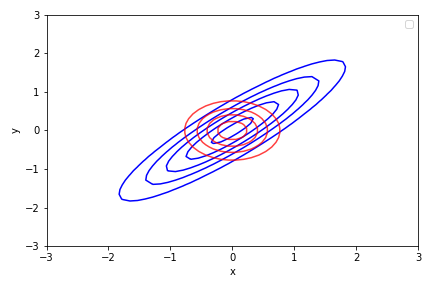
\includegraphics[width=0.3\textwidth]
		{figs/klil3a.png}}
	\subfloat[$D_{KL}(g||q)$]{\label{vixep1b}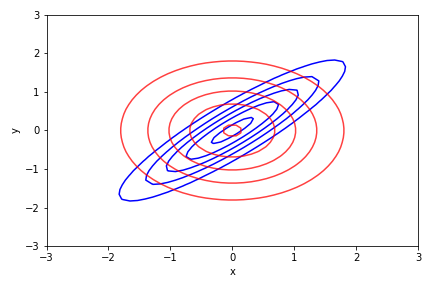
\includegraphics[width=0.3\textwidth]
		{figs/klil3b.png}}


	\caption[Difference of behavior when minimizing $D_{KL}(q||g)$ and $D_{KL}(g||q)$]{\label{vixepfigure} Difference of behavior when minimizing $D_{KL}(q||g)$ (a) and when minimizing $D_{KL}(g||q)$ (b). Here the true distribution (in blue) is approximated by a multivariate normal distribution with diagonal covariance (in red). Example inspired by \cite{Bishop_2007}. Generating code can be found in \url{https://github.com/DFNaiff/Dissertation/blob/master/illustrations_dissertation/kl_illustrative_2.py}.}
\end{figure}

\section{Mean field variational inference}
Traditionally, variational inference has mainly been concerned with factorized variational approximations of the form $q(\theta;\lambda) = \prod_{i=1}^D q_i(\theta_i;\lambda_i)$, called \textit{mean field approximation}. The use of such variational posterior greatly simplifies the optimization of ELBO by coordinate descent. 

To see this, consider a single term $j$ of the variational approximation $q(\theta) = \prod_{i=1}^D q_i(\theta)$. The ELBO for $q(\theta)$ is:
\begin{equation} \label{mfviexpansion}
\begin{split}
\mathcal{L}(q) & = \int \log \gu(\theta) \prod_{i=1}^D q_i(\theta_i) d \theta - \int \left(\sum_{j=1}^D \log q_i(\theta_i) \right) \prod_{i=1}^D q_i(\theta_i) d \theta \\
	     & = \int q_j(\theta_j) \left( \int \log \gu(\theta) \prod_{i \neq j} q_i(\theta_i) d \theta_i \right) d\theta_j + \sum_{i=1}^D \mathcal{H}(q_i) \\
	     & = \int q_j(\theta_j) \log \phi_j (\theta_j) d\theta_j + \mathcal{H}(q_j) + \sum_{i\neq j} \mathcal{H}(q_i),
\end{split}
\end{equation}
With
\begin{displaymath}
\log \phi_j(\theta_j) := \int \log(\gu(\theta)) q_{-j}(\theta_{-j}) d\theta_{-j} = \Ev_{\theta_{-j} \sim q_{-j}} [ \log \gu(\theta) ],
\end{displaymath}
using the notation $q_{-j}(\theta_{-j}) = \prod_{i\neq j}q_i(\theta_i)$.
Now, assuming $\exp ( \log \phi_j(\theta_j))$ to be integrable over the support of $g(\theta)$, fix every $q_i$ for $i \neq j$, so that the only term to be maximized is $q_j$. Then, maximizing \eqref{mfviexpansion} in respect to $q_j$ is equivalent to maximizing the ELBO between $q_j$ and $\exp \left(\log \phi_j(\theta_j)\right) $. Since there are not any constraints in the choice for $q_j$
\begin{equation} \label{mfviqj}
q^{*}_j(\theta_j;q_{-j}) \propto \exp \Ev_{\theta_{-j} \sim q_{-j}} [ \log \gu(\theta)].
\end{equation}
This readily gives an algorithm to find $q^* = \prod q^*_j$: initialize $q_1,\ldots,q_D$ in a appropriate manner, and then optimize cyclically \eqref{mfviqj}. 

Convergence is guaranteed due to the convexity of the bound with respect to each factor \cite{Bishop_2007,Boyd_2004}. This algorithm interacts well with target densities whose conditional distributions $g(\theta_j|\theta_{-j})$ belongs to the exponential family, that is, 
\begin{equation}\label{exponential_family}
 g(\theta_j|\theta_{-j}) = h(\theta_j) \exp \left( \eta_j(\theta_{-j})^T t(\theta_j) - a(\eta_j(\theta_{-j})) \right),
\end{equation}
\eqref{mfviqj} reduces to \cite{Blei_2017} 
\begin{equation}
 q^*_j(\theta_j;q_{-j}) \propto h(\theta_j) \exp \left( \Ev_{\theta_j \sim q_{-j}} [\eta_j(\theta_{-j})]^T t(\theta_{-j}) \right),
\end{equation}
thus if $\nu_j = \Ev_{\theta_{-j} \sim q_{-j}}[\eta_j(\theta_{-j})]^T$ is available analytically, the coordinate descent becomes relatively simple.

Research to extend mean field variational inference to large datasets or dimensionality exists \cite{Hensman_2012,Hoffman_2013,Zhang_2019}, however factorized limitations are limited, particularly in its independence assumption. Moreover, many distributions are not in the exponential family, which is the focus of the mean field method, so more generic methods are desirable.

\section{Generic variational inference}
Some recent advances in variational inference \cite{Zhang_2019} are concerned with expanding both the set of possible variational approximations $\mathcal{Q}$ and approximating general classes of posterior distributions $g(\theta)$. 

Considering again $\mathcal{Q}$ to be parameterized by a continuous set of parameters $\Lambda$, and using the overloaded notation $\mathcal{L}(\lambda) = \mathcal{L}(q(\cdot;\lambda))$, return to the optimization problem 
\begin{equation}
\begin{split}
\lambda^* = \argmax_{\lambda \in \Lambda} \mathcal{L}(\lambda) & = \argmax_{\lambda \in \Lambda} \left( \Ev_{\theta \sim q(\theta;\lambda)}[\log \gu(\theta)] + \mathcal{H}(q(\cdot;\lambda)) \right)\\
& =  \argmax_{\lambda \in \Lambda} \Ev_{\theta \sim q(\theta;\lambda)}\left[\log \left(\frac{\gu(\theta)}{q(\theta;\lambda)}\right)\right]
\end{split}
\end{equation}
In general the expectations involved cannot be calculated analytically. However, if one represents $\nabla \mathcal{L}(\lambda)$ as expectations, then by using Monte Carlo methods it is possible to use stochastic gradients methods \cite{Robbins_1951,Kingma_2014,Qian_1999,Ruder_2016} to maximize $\mathcal{L}(\lambda)$ \footnote{In this aspect, modern variational inference research benefits greatly from deep learning research, the later relying heavily on stochastic gradient descent, driving much of the recent development of these algorithms.}.

\subsection{REINFORCE}
One proposal for doing this is given in \cite{Wingate_2013} and \cite{Ranganath_2014}, where $\nabla \mathcal{L}(\lambda)$ is rewritten as \footnote{A quick derivation of this approximation is done in the Appendix \ref{appendixreinforce}.}
\begin{equation}\label{reinforce}
\nabla \mathcal{L}(\lambda) = \Ev_{\theta \sim q(\theta;\lambda)} \left[ \log \frac{\gu(\theta)}{q(\theta;\lambda)} \nabla_{\lambda} \log q(\theta;\lambda) \right], 
\end{equation}
and is approximated with its Monte Carlo estimator 
\begin{equation}\label{reinforcemc}
\nabla \mathcal{L}(\lambda) \approx \frac{1}{K} \sum_{i \in [K], \theta_i \sim q(\theta;\lambda)} \log \frac{\gu(\theta_i)}{q(\theta_i;\lambda)} \nabla_{\lambda} \log q(\theta_i;\lambda),
\end{equation}
where $[K] = \{1,\ldots,K\}$. In practice, this estimation suffers from high variance, which may hinder optimization. In \cite{Wingate_2013}, \eqref{reinforce} is substituted for 
\begin{equation}
\nabla \mathcal{L}(\lambda) = \Ev_{\theta \sim q(\theta;\lambda)} \left[ \left( \log \left( \frac{\gu(\theta)}{q(\theta;\lambda)}\right) + C\right) \nabla_{\lambda} \log q(\theta;\lambda) \right], 
\end{equation}
where $C$ is an arbitrary constant, which is adjusted to control variance \footnote{The reason that this constant can be added is because $\int C \nabla_\lambda \log q(\theta;\lambda) q(\theta;\lambda) d\theta = C \int \nabla_\lambda p(\theta;\lambda) d\theta = C \nabla_\lambda \int p(\theta;\lambda) d\theta = 0$.}. In \cite{Ranganath_2014}, the variance is controlled by Rao-Blackwellization and control variates instead. Other variance reduction methods for this gradient formulation are proposed in \cite{Titsias_2015} and \cite{Ruiz_2016}.

\subsection{Reparameterization trick}\label{reparameterizationsection}
An alternative to calculate the gradient of $\mathcal{L}(\lambda)$ as an expectation is known as the \textit{reparameterization trick} \cite{Kingma_2013}, which is a general technique for calculating gradients of expectations of continuous random variables.

To explain the general ideia, assume $X_\lambda$ is a continuous random variable distributed according to $f(x;\lambda)$, and one wants to calculate the gradient (in relation to $\lambda$) of
\begin{equation}\label{reparamderiv1}
\Ev_{X_\lambda} \left[ h(X_\lambda) \right] = \int h(x) f(x;\lambda) dx.
\end{equation}
We approximate \eqref{reparamderiv1} by Monte Carlo
\begin{equation}\label{reparamderiv2}
\Ev_{X_\lambda} \left[ h(X_\lambda) \right] \approx \sum_{i=1}^N h(x_{i,\lambda}), \quad x_{i,\lambda} \sim f(x;\lambda).
\end{equation}
Now suppose that there is some random variable $Y$, \textit{not depending on $\lambda$}, with density $r(y)$, such that $X_\lambda = s(Y;\lambda)$ (for instance, if $X_{\mu,\sigma} \sim \mathcal{N}(\mu,\sigma^2)$, then being $Y \sim \mathcal{N}(0,1)$, we have that $X_{\mu,\sigma} = s(Y;\mu,\sigma) = \sigma Y + \mu$). In this case, the Monte Carlo estimator \eqref{reparamderiv2} is rewritten as
\begin{equation}
\Ev_{X_\lambda} \left[ h(X_\lambda) \right] \approx \sum_{i=1}^N h(s(y_i,\lambda)), \quad y_i \sim r(y),
\end{equation}
which is an expression \textit{whose gradient in relation to $\lambda$ can be taken}, and is the Monte Carlo estimator of
\begin{equation}
\int h(s(y;\lambda)) r(y) dy = \Ev_Y [h(s(Y;\lambda))]
\end{equation}

Formally, by letting $A$ be the support of $Y$ and $B_\lambda$ be the support of $X_\lambda$, if $s(y;\lambda)$ if bijective with injective derivative:
\begin{equation}
\begin{split}
\Ev_{X_\lambda \sim f(x;\lambda)} [h(x)] & = \int_{B_\lambda} h(x) q(x;\lambda) dx \\
& = \int_A h(s(y;\lambda)) q(s(y;\lambda);\lambda) |\text{det} (s'(y;\lambda))| dy \\
& = \int_A h(s(y;\lambda)) r(y) dy = \Ev_{Y \sim r(y)} [h(s(y;\lambda))],
\end{split}
\end{equation}
which shows that the reparameterization trick is valid.

To apply this to $\mathcal{L}(\lambda)$, assume $\theta_\lambda \sim q(\theta;\lambda)$ is such that $\theta_\lambda = s(\epsilon;\lambda)$, with $\epsilon \sim r(\epsilon)$. Then, applying reparameterization, we have
\begin{equation}\label{mcreparameterization}
\begin{split}
 \nabla \mathcal{L}(\lambda) & = \nabla \left(\Ev_{\theta \sim  q(\theta;\lambda)}\left[\log \frac{\gu(\theta)}{q(\theta;\lambda)}\right] \right) \\
 & =\nabla \left( \Ev_{\epsilon \sim r(\epsilon)} \left[\log \frac{ \gu(s(\epsilon;\lambda))}{q(s(\epsilon;\lambda);\lambda)}\right]\right) \\
 & \approx \nabla_\lambda \left( \frac{1}{K} \sum_{i \in [K], \epsilon_i \sim r(\epsilon)} \log \frac{ \gu(s(\epsilon_i;\lambda))}{q(s(\epsilon_i;\lambda);\lambda)} \right)
\end{split}
\end{equation}
In \cite{Zhang_2019}, it is argued that the observed lower variance of this estimation methods, if compared to the one given by \eqref{reinforce}, may be due to the fact that reparameterization trick takes in account the gradient of the target distribution, instead of just the gradient of the variational distribution as in \eqref{reinforce}. Moreover, in cases that the entropy of $q(\cdot;\lambda)$ can be estimated analytically, the reparameterization trick can be applied only to $\gu(\theta)$, leading to lower variance. Finally, it is important to notice that this format is more readily integrated in an automatic differentiation package, since it suffices to calculate the sum inside the gradient and backpropagate it in relation to $\lambda$.

\iffalse
These recent advances in the field, allowing the application of variational inference for a general variety of target distributions, has resulted in the technique return to some popularity, with recent probabilistic programming language focusing on it, such as Pyro \cite{Bingham_2018} and Edward \cite{Tran_2016}.
\fi

\section{Mixtures of gaussians for variational approximations}\label{mixgaussiansvi}

The idea of using mixture distributions for variational inference dates back to the late 90s \cite{Bishop_1997,Jaakkola_1998}, originally developed for a limited number of target distributions, and later is explored for approximating general distributions in \cite{Gershman_2012,Salimans_2012}, leading to recent work in it \cite{Acerbi_2018,Arenz_2018,Guo_2016,Jankowiak_2019,Miller_2016}. The technique presented here uses the reparameterization trick, in a vein similar to the one presented in \cite{Miller_2016}. In general, the mixture distribution considered is one of Gaussian distributions (as it is in this work), although many of those extends to more general mixtures.

More formally, consider as the set of candidate proposals 
\begin{equation}
\mathcal{Q}_k := \left\{\sum_{i=1}^k w_i f(\cdot;\lambda_i) \middle| f(\cdot;\lambda_i) \in \mathcal{Q}_1, 1 \leq i \leq k; (w_1,...,w_k) \in \Delta_k \subset \mathbb{R}^k \right\},
\end{equation}
wher $\Delta_k$ denotes the probability simplex $\{(x_1,\ldots,x_k) \in {\mathbb{R}^+}^k| \sum_{i=1}^k x_k = 1\}$, and $\mathcal{Q}_1 = \{f(\cdot;\lambda) | \lambda \in \Lambda \subset \mathbb{R}^m\}$ is a parameterized set of distributions. In the mixture of multivariate normals case,
\begin{equation}
\mathcal{Q}_1 := \{f(\cdot ; \mu,\Sigma) = \mathcal{N}(\cdot;\mu,\Sigma) | \mu \in \mathbb{R}^d,\Sigma \in \mathbb{R}^{d \times d}, \Sigma \geq 0\} 
\end{equation}
is the set of multivariate normal distributions. In many cases, it is interesting to restrict $\mathcal{Q}_1$ further so that $\Sigma$ is diagonal.
Mixtures of distributions are interesting as variational approximations since their expectations are easily available 
\begin{equation}
\Ev_{X \sim \sum_i w_i f_i} [h(X)] = \sum_i w_i \Ev_{X_i \sim f_i} [h(X_i)],
\end{equation}
as well as their covariances
\begin{equation}
\begin{split}
& \Cov_{X \sim \sum_i w_i f_i}(X) = \sum_i w_i \left( \Sigma_i +   \mu_i \mu_i^T \right) - \mu \mu^T, \\
& \Sigma_i = \Cov_{X_i \sim f_i}(X_i), \quad \mu_i = \Ev_{X_i \sim f_i}[X], \quad \mu = \Ev_{X \sim \sum_i w_i f_i} [X].
\end{split}
\end{equation}
Furthermore, samples of mixtures can be easily generated from the base distributions, by choosing mixture $i$ with probability $w_i$, and then sampling $X$ from $f(\cdot;\lambda_i)$ \footnote{Batching this process in order to sample many variables, escaping loops in interpreted languages with support for numerical operations (such as Python with Numpy) requires some care, but it is possible in few lines.}. Furthermore, letting $\mathcal{Q}_\infty = \cup_{i=1}^\infty \mathcal{Q}_i$ and $\mathcal{Q}_1$ be these set of Gaussian distributions, $\mathcal{Q}_\infty$ is dense in the set of continuous distributions \cite{Epanechnikov_1969}, so in this case any continuous distribution can be approximated arbitrarily close, in principle.

Considering mixtures of Gaussians, for fixed $k$, in order to find the parameters
\begin{displaymath} 
\lambda = (w_1,\mu_1,\Sigma_1,\ldots,w_k,\mu_k,\Sigma_k)
\end{displaymath}
of 
\begin{equation}
 q^*_k = \argmax_{q_k \in \mathcal{Q}_k} \mathcal{L}(q_k),
\end{equation}
one needs first to find suitable parameterizations for $\Sigma_i$ and $\mathbf{w} := (w_1,...,w_k)$. For the covariance matrix, one can either consider only diagonal matrices
\begin{equation}
\Sigma_i = \text{diag}(\sigma^2_{i,1},\ldots,\sigma^2_{i,D}),
\end{equation}
or consider matrices of the form
\begin{displaymath}
 \Sigma_i = \u_i \u_i^T + \text{diag}(\sigma^2_{i,1},\ldots,\sigma^2_{i,D}),
\end{displaymath}
or use more advanced parameterizations such as the ones found in \cite{Pinheiro_1996}. Let $\sigma_i$ be the parameters for $\Sigma_i$, so that $\Sigma_i = \Sigma_i(\sigma_i)$. For $\mathbf{w}$, using some monotone bijective differentiable function $\phi : \mathbb{R} \to \mathbb{R}^+$ (for example, $\phi = \exp$), one can then consider the corresponding differentiable map $\Phi : \mathbb{R}^k \to \Delta_k$ as 
\begin{equation}
\Phi(\nu_i) = \frac{\phi(\nu_i)}{\sum_{i=1}^k \phi(\nu_k)} = w_i(\nu_i).
\end{equation}

The parameter of interest $\lambda$ becomes $(\nu_1,\mu_1,\sigma_1,\ldots,\nu_k,\mu_k,\sigma_k)$, and
\begin{equation}
q_k(\theta) = \sum_{i=1}^k w_i(\nu_i) f_{\mathcal{N}(\mu_i,\Sigma(\sigma_i))}(\theta).
\end{equation}
Thus, the ELBO objective becomes
\begin{equation}\label{elbomixturegaussians}
\begin{split}
\mathcal{L}(\lambda) & = \int \log \gu(\theta) q_k(\theta) d\theta - \int \log (q_k(\theta)) q_k(\theta) d \theta \\
& = \sum_{i=1}^k w_i(\nu_i) \Ev_{\theta_i \sim \mathcal{N}(\mu_i;\Sigma(\sigma_i))}\left[\log \frac{ \gu(\theta_i)}{q_k(\theta_i;\lambda)}\right].
\end{split}
\end{equation}

One can adapt the reparameterization trick to rewrite $\mathcal{L}(\lambda)$ in a manner suitable to stochastic gradient optimization. First notice that any gaussian random variable $X \sim \mathcal{N}(\mu,\Sigma)$ can be written as $X = \mu + A Z$, where $Z \sim \mathcal{N}(0,I)$ and $A$ is some matrix such that $\Sigma = A A^T$. For instance, $A$ can be the lower Cholesky factor of $\Sigma$, if the parameterization of $\Sigma$ only supports positive-definite matrices. Then $A(\sigma)$ is differentiable \cite{Smith_1995,Murray_2016}, and $s(\epsilon;\mu_i,\sigma_i) = \mu_i + A(\sigma) \epsilon$, and \eqref{elbomixturegaussians} is approximated by Monte Carlo,
\begin{equation}\label{mcmixturegaussians}
\begin{split}
\mathcal{L}(\lambda) & = \sum_{i=1}^k w_i(\nu_i) \Ev_{\epsilon \sim \mathcal{N}(0,I)}\left[\log \frac{ \gu(s(\epsilon;\mu_i,\sigma_i))}{q_k(s(\epsilon;\mu_i,\sigma_i);\lambda)}\right] \\
& \approx \sum_{i=1}^k w_i(\nu_i) \left( \frac{1}{K_i} \sum_{k \in [K_i], \epsilon_{i,j} \sim \mathcal{N}(0,I)} \log \frac{ \gu(s(\epsilon_{i,j};\mu_i,\sigma_i))}{q_k(s(\epsilon_{i,j};\mu_i,\sigma_i);\lambda)} \right),
\end{split}
\end{equation}
which is an expression that can be differentiated to find an approximation for $\nabla \mathcal{L}(\lambda)$.

In principle there is no way to know how many mixtures are necessary to return a good approximation. However, one can,for each $i \in \mathbb{N}$, starting with $i = 1$, sequentially find $q^*_i$ close to $\argmax_{q_i \in \mathcal{Q}_i} \mathcal{L}(q)$, and go to sequentially from $Q_i$ to $Q_{i+1} \supset Q_i$, until the variational approximation is good enough. However, this procedure runs into computational issues, namely the number of optimization parameters scale linearly with the number of mixtures $k$, in a non-convex problem with non-trivial gradient evaluation, whose cost also scales linearly with $k$. Hence, the cost of improving the mixtures this way quickly becomes rather large. We next present an approach that mitigates this problem, at the cost of making a greedy approximation, thus potentially more inefficient in the number of mixtures.

\subsection{Boosting mixtures of gaussians}\label{boostedvi_section}
Boosting \cite{Freund_1997,Freund_1999,Friedman_2000} is a standard technique in machine learning, usually used in classification problems, which tries to combine slighty better than chance algorithms, or \textit{weak learners} in a reliable, accurate algorithm (a \textit{strong learner}). The general framework is transferred to the problem of variational inference in concurrent works by \cite{Miller_2016} and \cite{Guo_2016}, using increasing mixtures distributions.

In this setting, start first with some distribution $q_1 \in \mathcal{Q}_1$. Then, recursively, given a proposal $q_{i-1}^*$,  it is considered the proposal set
\begin{equation}
\begin{split}
\mathcal{Q}_{i} = \mathcal{Q}_{i}(q_{i-1}) = \{ (& 1-w_{i}) q_{i-1} + w_{i}  f(\cdot;\mu_{i},\Sigma_{i}) | \\  & w_i \in [0,1], \mu_i \in \mathbb{R}^d, \Sigma_i \in \mathbb{R}^{d \times d}, \Sigma_i \geq 0\},
\end{split}
\end{equation}
and then some $q_i$ is chosen from $\mathcal{Q}_i$, in a manner that $\mathcal{L}(q_i)$ is reasonably greater than the previous value $\mathcal{L}(q_{i-1})$. One straightforward approach is to seek $\lambda_i (w_{i}^*,\mu_{i}^*,\Sigma_{i}^*)$ such as the maximization objective becomes
\begin{equation}\label{miller_objective}
 \mathcal{L}_{i}(\lambda_{i}) := \mathcal{L}((1-w_{i}) q_{i-1} + w_{i}  f(\cdot;\mu_{i},\Sigma_{i})),
\end{equation}
which is the procedure proposed in \cite{Miller_2016}. In \cite{Guo_2016}, it is shown that the KL divergence satisfies the conditions estabilished by \cite{Tong_Zhang_2003} that ensures if
\begin{equation}
 \mathcal{L}((1-w_i){i-1} + w_i f_i) \geq \sup_{f \in Q_1,w\in[0,1]} \mathcal{L}((1-w)q_{i-1} + w f) - \epsilon_i,
\end{equation}
as $\epsilon_i \to 0$, then
\begin{equation}
 \lim_{i \to \infty} \sup_{q \in Q_\infty} L(q) - \mathcal{L}(q_i) = 0,
\end{equation}
provided that every $q \in \mathcal{Q}_1$ is bounded from below. In \cite{Guo_2016}, it is shown that the KL divergence satisfies those two conditions, if every $q \in \mathcal{Q}_1$ is assumed to be bounded from below by a positive constant. Although this is not the case for Gaussian distributions, it is argued that since in actual implementations the practitioner works with a bounded set of interest, the result holds in practice.

\subsection{Gradient boosting mixture of gaussians}\label{gradboostsection}
Another boosting proposal, due to \cite{Guo_2016}, is to instead of trying to optimize jointly $(w_{i}^*,\mu_{i}^*,\Sigma_{i}^*)$ at each step, choosing first $f_{i} = f(\cdot;\mu_{i},\Sigma_{i})$, and then choose $w_i$ as to maximize:
\begin{equation}\label{boosting_objective_alpha}
\begin{split}
 \mathcal{L}_{i}(w_{i}) & := \mathcal{L}((1-w_{i}) q_{i-1} + w_{i}  f_{i}) \\
 & = \int \log \frac{\gu(\theta)}
				 {(1-w_{i}) q_{i-1}(\theta) + w_{i} f_{i}(\theta)} ((1-w_{i}) q_{i-1}(\theta) + w_{i} f_{i}(\theta)) d\theta.
 \end{split}
\end{equation}
Since the KL divergence is convex in $q$, the ELBO is concave, so minimizing $w$ is easy, provided we can easily calculated $\mathcal{L}'_i(w_i)$. Since we have 
\begin{equation}\label{boosting_objective_dalpha}
\begin{split}
 \mathcal{L}'_{i}(w_{i}) & = 
	 \int \frac{\partial}{\partial w_{i}} \left( \log  \frac{\gu(\theta)}
	 {(1-w_{i}) q_{i-1}(\theta) + w_{i} f_{i}(\theta)} ((1-w_{i}) q_{i-1}(\theta) + w_{i} f_{i}(\theta))\right) d\theta \\
	 & = \int \log (\gu(\theta)) (f_{i}(\theta) - q_{i-1}(\theta)) d\theta - \\
	 & \qquad{} \int \log((1-w_{i}) q_{i-1}(\theta) + w_{i} f_{i}(\theta)) (f_i(\theta) - q_{i-1}(\theta)) d\theta,
\end{split},
\end{equation}
we can then approximate the derivative by Monte Carlo
\begin{equation}
\begin{split}
\mathcal{L}'_i(w_i) = & \frac{1}{J} \sum_{j \in [J] \theta_{j} \sim f_i} \left(\log(\gu(\theta_j)) - \log((1-w_{i}) q_{i-1}(\theta_j) + w_{i} f_{i}(\theta_j))\right) \\
& -\frac{1}{K} \sum_{\theta_{k} \in [K], \theta_k \sim q_{i-1}} \left(\log(\gu(\theta_k)) - \log((1-w_{i}) q_{i-1}(\theta_k) + w_{i} f_{i}(\theta_k))\right),
\end{split}
\end{equation}
and using it to maximize $\mathcal{L}'_i(w_i)$.

The question becomes then how to choose $f_i$. In \cite{Guo_2016}, the technique of gradient boosting \cite{Friedman_2001} is borrowed for this purpose, so that $f_i$ is chosen as to minimize $\nabla D_{KL} (q_{i-1}||g)  \cdot f$, where $\nabla D_{KL}(q || g)$ is the functional derivative of $D_{KL}(q || g)$ as a function of $q$. For $D_{KL}(q || p)$, we can use Taylor expansion to find the functional derivative
\begin{equation}
\begin{split}
 D_{KL}(q + \delta h || p) & = \int (q + \delta h) \log \frac{q + \delta h}{p} \\
					  & = \int q \left(\log \frac{q}{p} + \frac{\delta h/p}{q/p} + \mathcal{O}(\delta^2) \right) + \delta \int h \log \frac{q}{p} + \mathcal{O}(\delta^2) \\
					  & = D(q||p) + \delta \int \left(1 + \log \frac{q}{p}\right) h + \mathcal{O}(\delta^2).
\end{split}			  
\end{equation}
Here the argument $\theta$ is omitted to simplify the expression. Hence 
\begin{equation} \label{idealklgrad}
\begin{split}
f_i = \argmin_{f} \nabla D_{KL}(q_{i-1} || g) \cdot f & = \argmin_{f} \int \left(1 + \log \frac{q_{i-1}(\theta)}{g(\theta)}\right) f(\theta) d \theta = \\
& = \argmin_{f} \int \log \frac{q_{i-1}(\theta)}{g(\theta)} f(\theta) d\theta.
\end{split}
\end{equation}

Since the parameterization for $f_i(\theta)$ allows degeneration to a point mass at $\argmin_{\theta} \log (q_{i-1}(\theta) / g(\theta))$, and this point mass optimizes \eqref{idealklgrad}, further constraints over $f_i(\theta)$ are needed for getting a non-degenerate new basis function. In \cite{Guo_2016} \eqref{idealklgrad} is regularized by the logarithm of the $L_2$ norm of $f_i(\theta)$
\begin{equation}
f_i =  \argmin_{f} \left( \int \log \frac{q_{i-1}(\theta)}{g(\theta)} f(\theta) d\theta +  \frac{\lambda}{2} \log ||f||_2^2 \right)
\end{equation}
while in \cite{Locatelo_2018}, \eqref{idealklgrad} is regularized by negative of the entropy of $f$, as a proxy for the regularization of its $L_\infty$ norm. Since for $f(\theta) = \mathcal{N}(\theta|\mu,\Sigma)$, $\log ||f||_2^2 = -\frac{1}{2} \log |\Sigma| - \frac{1}{2} \log(2\pi)$ and $-\mathcal{H}(f) = -\frac{1}{2} \log |\Sigma| - \frac{1}{2} \log(2\pi e)$, both approaches are equivalent for mixture of Gaussians, yielding the maximization objective in relation to $\mu_i,\Sigma_i$:
\begin{equation}\label{relbogaussian}
\begin{split}
 \text{RELBO}(\mu_i,\Sigma_i) = & \int \log(\gu(\theta)) \mathcal{N}(\theta|\mu,\Sigma) d\theta - \int \log(q_{i-1}(\theta)) \mathcal{N}(\theta|\mu,\Sigma) d\theta + \\
 & \frac{\lambda}{4} \log |\Sigma|,
 \end{split}
\end{equation}
where $\lambda$ is a regularization constant (the name RELBO comes from \cite{Locatelo_2018}). This constant may be set either as a fixed value or decaying as $i$ increases, as to permit increasingly narrower distributions as the algorithm runs. For example, in \cite{Locatelo_2018} $\lambda$ is set as $1/\sqrt{i+1}$. \footnote{In \cite{Guo_2016} it is argued that this objective is still somewhat hard to maximize, so it is proposed an heuristic based on a local Laplace approximation. This heuristic was previously explored by the author of this work, however it ran into implementation issues, and moreover, it does not exactly attend the desiderata in this work, namely as few function evaluations as possible}. Finally, the gradients of \eqref{relbogaussian} in relation to $\mu_i,\Sigma_i$ can be estimated by the reparameterization trick. 

The resulting pseudo-algorithm is shown in Figure \ref{vbalgorithm}.
\begin{Algorithm}
\begin{algorithmic}[1]\label{vbalgorithm}
\Procedure{VariationalBoosting}{$\log \gu,\mu_0$,$\Sigma_0$}
\LineComment{$\mu_0,\Sigma_0$ the are initial boosting values}
\State $w_0 := 1.0$
\For{$t=1,...,T$}
	\State $\mu_{t},\Sigma_{t} := \argmax RELBO(\mu_{t},\Sigma_{t})$ \Comment{Using reparameterization}
	\State $w_{t} := \argmax \mathcal{L}_i(w_i)$ \Comment{Using $\mathcal{L}'_t(w_t)$ for gradient descent}
	\For{$j=0,...,t-1$}
		\State $w_{j} \gets (1-w_t)w_j$
	\EndFor
\EndFor
\State \Return $\{(\mu_t,\Sigma_t,w_t)\}_{t=1}^T$
\EndProcedure
\end{algorithmic}
\caption{\label{vbalgorithm}Variational boosting algorithm.}
\end{Algorithm}

\section{Using Bayesian Monte Carlo in Variational Inference}\label{vbmc_section}

All the approaches previously presented suffers from one major flaw: the need for a large number of evaluations of the unnormalized posterior $\gu$ by Monte Carlo methods, in order to have a good estimation of the gradient. This is the same problem of integration that Bayesian Monte Carlo tries to solve, so one can try to use this technique when $\gu$ is expensive to evaluate. In \cite{Acerbi_2018}, it is developed a method called Variational Bayesian Monte Carlo (VBMC) that hinges on exactly this idea.

Consider a parameterized variational proposal $q(\theta;\lambda)$, and the corresponding ELBO for $\gu(\theta)$:
\begin{displaymath}
 \mathcal{L}(\lambda) = \mathcal{L}_\gu(\lambda) = \int \log \gu(\theta) q(\theta;\lambda) d\theta - \int \log(q(\theta;\lambda)) q(\theta;\lambda) d\theta.
\end{displaymath}
As in Chapter 4, setting as prior for $\log \gu(\theta)$ the Gaussian process $GP(m,k)$, and given set of evaluations $\mathcal{D}_0 = \{(x_i,f(x_i))\}_{i=1}^N$, $\mathcal{L}_\gu(\lambda)$ can be replaced by the Gaussian distributed random variable
\begin{equation}\label{vbmc_rvs}
\begin{split}
\mathcal{L}_\mathcal{D}(\lambda) := \mathcal{L}_{\gu_\mathcal{D}}(\lambda) &:= Z_\mathcal{D}(\lambda) - \int \log(q(\theta;\lambda)) q(\theta;\lambda) d\theta, \\
Z_\mathcal{D}(\lambda) & := \int \log \gu_\mathcal{D}(\theta) q(\theta;\lambda) d\theta,
\end{split}
\end{equation}
with mean
\begin{equation}
\begin{split}
\bar{\mathcal{L}}_\mathcal{D}(\lambda) := \Ev \left[ \mathcal{L}_{\log \gu_\mathcal{D}}(\lambda) \right] & = \Ev[Z_\mathcal{D}(\lambda)] - \int \log(q(\theta;\lambda)) q(\theta;\lambda) d\theta \\
& = \int \Ev[\log \gu_\mathcal{D}(\theta)] q(\theta;\lambda) d\theta - \int \log(q(\theta;\lambda)) q(\theta;\lambda) d\theta\\
& = \mathcal{L}_{\Ev[\log \gu_\mathcal{D}]} (\lambda), \\
\end{split}
\end{equation}
and variance
\begin{equation}
\Var(\mathcal{L}_\mathcal{D}(\lambda)) = \Var(Z_\mathcal{D}(\lambda)),
\end{equation}
and $\Ev[Z_\mathcal{D}(\lambda)]$ and $\Var[Z_\mathcal{D}(\lambda)]$ being given by \eqref{evvarbmc2}.
This approach enjoy the same benefits as the BMC approach:
\begin{itemize}
	\item If the evaluation of $\gu$ is expensive, it is not feasible to perform a Monte Carlo estimation of $\int \log \gu(\theta) q (\theta;\lambda) d \theta$ at each step in optimizing the ELBO.
	\item The function $\gu$ does not need to be differentiable, and its evaluations may be noisy (although this last case is not considered in this work, the extension is straightforward).
\end{itemize}
In case $q(\theta;\lambda)$ is a mixture of $i$ Gaussians $q_i(\theta;\lambda)$, as in \cite{Acerbi_2018}, the methods presented in \ref{mixgaussiansvi} and the one in Chapter 4, by the discussion in Section \ref{kerneldistributionbmc}, given a suitable kernel $k$, $\Ev[Z_\mathcal{D}(\lambda)]$ and $\Var[Z_\mathcal{D}(\lambda)]$ can be easily treated. In \cite{Acerbi_2018}, $k$ is the SQE kernel \eqref{sqekernel} with outputscale $r_0$ and lengthscales $l_1,\ldots,l_D$, which by \eqref{bmcmixgaussians} makes $\Ev[Z_\mathcal{D}(\lambda)]$ and $\Var[Z_\mathcal{D}(\lambda)]$ both analytical.

The entropy term $-\int \log(q(\theta;\lambda)) q(\theta;\lambda) d\theta$ does not have in general a closed form, and must still be treated. Approximating $-\log(q(\theta;\lambda))$ by BMC is possible, but since this term changes with $\lambda$, this will be costly. However, since $\log q(\theta;\lambda)$ is easy to evaluate, by construction, the entropy term can be treated with the reparameterization trick without much additional cost. Other possible approach to deal with this term, when using mixture of Gaussians, is to use one of the approximations proposed in \cite{Huber_2008}. 

An important point is that, since, by in the first equation of \eqref{evvarbmc2}, only $\mathbf{z}$ and $\int m(\theta) q(\theta;\lambda) d\theta$ depends on $q(\theta;\lambda)$, one can rewrite
\begin{equation}
\begin{split}
\int \Ev[\log \gu_\mathcal{D}(\theta)] q_k(\theta;\lambda) d\theta & = M(\lambda) + \mathbf{z}^T \mathbf{w} \\
\mathbf{w} & = K^{-1} \mathbf{y} \\
M(\lambda) & = \int m(\theta) q(\theta;\lambda) d\theta \\
\mathbf{z}_i & = \int k(x,x_i) q(\theta;\lambda) dx.
\end{split}
\end{equation}
This way, with $\mathbf{w}$ being previously computed, the computation of $\bar{\mathcal{L}}_\mathcal{D}(\lambda)$ can be calculated in $\mathcal{O}(N)$ time for each $\lambda$, while $\Var(\mathcal{L}_\mathcal{D}(\lambda))$ can be calculated in $\mathcal{O}(N^2)$. The new variational objective becomes then simply $\bar{\mathcal{L}_\mathcal{D}}(\lambda)$.

\subsection{Quadratic mean function}\label{quadmeanfnsection}
With the objective $\bar{\mathcal{L}}_\mathcal{D}(\lambda)$, the actual distribution that is being approximated by mixture of Gaussians is proportional to $\exp \Ev[\log \gu_\mathcal{D}(\theta)]$. From the variational inference approximation's point of view, the only information that it has on the original distribution $\gu$ is by its GP approximation. 

This raises some issues: if the mean function of the GP prior $m(\theta)$ is either zero or a constant, and the kernel is one that decays to zero as $|x - x'|$ goes to infinity, such as \eqref{sqekernel}, \eqref{maternkernel} or \eqref{spectralmixturekernel}, then $\exp \Ev[\log \gu_\mathcal{D}(\theta)]$ is not integrable, so it cannot define an unnormalized probability distribution. Hence, care must be taken with the mean function $m(\theta)$.

One approach is to simply let $m(\theta)$ have a very low value, so that in practice it resembles enough a probability distribution so that, for a reasonable number of mixtures $k$, convergence issues does not appear. This is the default approach used in the developed algorithm presented in Chapter 4. An alternative approach, used in \cite{Acerbi_2018}, is to change the mean function so that $\exp(m(\theta))$, thus $\exp \log \Ev[\log \gu_\mathcal{D}(\theta)]$ is an unnormalized probability distribution, while having the integral $\int m(\theta) q_k(\theta) d \theta$ being analytically tractable. In \cite{Acerbi_2018}, the following mean function is proposed:
\begin{equation}\label{vbmc_quadratic_mean}
 m_{Q}(\theta;l,c) = - \frac{1}{2} \sum_{i=1}^D \frac{(\theta_i - c_i)^2}{l_i^2},
\end{equation}
which then both makes $\exp(m_Q(\theta;l,c))$ integrable and yields, for $q_i(\theta)$ being a mixture of Gaussians, 
\begin{equation}
 \int m_{Q}(\theta;l,c) q_k(\theta) d\theta = 
 	-\frac{1}{2} \sum_{j=1}^k \sum_{i=1}^D \left[\frac{(c_i - \mu_{k,i})^2}{l_i^2} + \frac{\Sigma_{k,i,i}}{l_i^2} \right].
\end{equation}
This comes immediately from the expectation of quadratic forms of normal distribution formula \cite{Petersen_2012}. 

\subsection{Remarks on acquisition functions for VBMC}
As in Bayesian Monte Carlo, a question that arises is one of active sampling. Notice that, fixed evaluations $\mathcal{D}$, and assuming a fixed set of mixtures of $k$ Gaussians $\mathcal{Q}_k$, associated with a fixed set of parameters $\Lambda_k$, and letting
\begin{equation}
\lambda^*(\mathcal{D}) = \argmin_{\lambda} \mathcal{L}_\mathcal{D}(\lambda),
\end{equation}
the final ELBO is a random variable $\mathcal{L}_{\mathcal{D}}(\lambda^*(\mathcal{D}))$, which is normally distributed with variance $\Var(Z_\mathcal{D}(\lambda^*))$. Since we want to have a high degree of certainty about the variational approximation's quality, one wants the final ELBO objective to have as lower variance as possible, since it is a measure of its uncertainty.

In this setting, one option would be, in a greedy approach, to choose $x_{N+1}$, so that, expanding $\mathcal{D}$ to $\mathcal{D}'(x,\log \gu(\theta_{N+1})) = \mathcal{D} \cup \{(x_{N+1},\log \gu(\theta_{N+1}))\}$, it minimizes the variance of $\mathcal{L}_{\mathcal{D'}}(\lambda^*(\mathcal{D'}))$. Since $\log \gu(\theta_{N+1})$ is not known in advance, one could substitute this instead for
\begin{equation}
\begin{split}
 & \Ev_\mathcal{D'} \left[ \Var(Z_{\mathcal{D'}}(\lambda^*(\mathcal{D'})) \right] \\
 & \mathcal{D}' = \mathcal{D} \cup \{(\theta_{N+1},\log \gu_\mathcal{D}(\theta_{N+1}))\}.
 \end{split}
\end{equation}
However, it is not clear how to work with this random variable, and minimize a measure of its uncertainty. However, this intuition helps with constructing heuristic acquisition functions to seek $\theta_{N+1}$.

\subsubsection{Uncertainty sampling and prospective prediction}
One option in order to tackle this problem is to consider the current variational proposal $q_k(\theta;\lambda)$ fixed, and consider the minimization objective
\begin{equation} 
 \alpha^\mathcal{D}_\text{VR}(\theta_{N+1}) = \Var\left(Z_{\mathcal{D}'(\theta_{N+1})}(\lambda)\right).
\end{equation}
However, since this is an expensive minimization objective, a proxy for this approach is to consider the integrand of
\begin{displaymath}
 \int \log \gu_\mathcal{D}(\theta) q_k(\theta;\lambda) d\theta,
\end{displaymath}
and seek the integrand maximum variance instead, resulting in the \textit{uncertainty sampling} maximization objective
\begin{equation}\label{us_vbmc}
 \alpha^\mathcal{D}_{\text{US}}(\theta_{N+1}) = k_\mathcal{D}(\theta_{N+1},\theta_{N+1}) q_k(\theta_{N+1};\lambda)^2.
\end{equation}

The above objective puts much weight in the current variational proposal, which may hinder exploration. Considering that future proposals will seek regions with high posterior density, the other objective proposed in \cite{Acerbi_2018} is formed by multiplying $\alpha^\mathcal{D}_{\text{US}}(\theta_{N+1})$ by an exploration factor for high posterior denstiies  $\exp(m_\mathcal{D}(\theta_{N+1}))$. This result in the \textit{prospective prediction} maximization objective,
\begin{equation}\label{prospective_vbmc}
\alpha^\mathcal{D}_{\text{PROP}}(\theta_{N+1}) = k_\mathcal{D}(\theta_{N+1},\theta_{N+1}) \exp(m_\mathcal{D}(\theta_{N+1}))q_k(\theta_{N+1};\lambda)^2.
\end{equation}
It is reported in \cite{Acerbi_2018} that the prospective prediction objective results in better approximations than the uncertainty sampling one. The objectives \eqref{us_vbmc} and \eqref{prospective_vbmc}, along with some newly proposed ones (\eqref{soft_prospective_vbmc},\eqref{mmlt_vbmc} and \eqref{mmltprop_vbmc}), are used in the algorithm developed in this work, to be shown in the next chapter.





\chapter{Boosted Variational Bayesian Monte Carlo}

In this chapter, it is presented a modification of the Variational Bayesian Monte Carlo approach presented in Section \ref{vbmc_section}, using ideas of boosting presented in \ref{boostedvi_section}, along with some other minor modifications of the previous approach.

\section{Boosting Variational Bayesian Monte Carlo}

The idea underlying this approach is rather simple: instead of using a GP surrogate model for doing variational inference with mixtures of Gaussians as in \ref{vbmc_section}, use it for variational inference with the gradient boosting approach discussed in section \ref{boostedvi_section}.

To expand on this, consider again the algorithm in Figure \ref{vbalgorithm}. In line 5, the objective \eqref{relbogaussian} (here called \textit{$f$-step}) consists of three terms
\begin{displaymath}
 \begin{split}
 \text{RELBO}(\mu_i,\Sigma_i) = & \int \log(\gu(\theta)) \mathcal{N}(\theta|\mu,\Sigma) d\theta \\
 & - \int \log(q_{i-1}(\theta)) \mathcal{N}(\theta|\mu,\Sigma) d\theta \\
 & + \frac{\lambda}{4} \log |\Sigma|,
 \end{split}
\end{displaymath}
while in line 6, for the objective \eqref{boosting_objective_alpha} (here called \textit{$w$-step}), the gradient $\mathcal{L}'_i(w_i)$ consists of
\begin{displaymath}
\begin{split}
 \mathcal{L}'_i(w_i) = & \int \log (\gu(\theta)) f_{i}(\theta) \\ 
 & -\int \log(\gu(\theta)) q_{i-1}(\theta)\\
 & + \int \log((1-w_{i}) q_{i-1}(\theta) + w_{i} f_{i}(\theta)) (f_i(\theta) - q_{i-1}(\theta)) d\theta
\end{split}
\end{displaymath}

Then, in the same vein of the VBMC method, set a $GP(m,k)$ prior for $\log \gu$, and given evaluations $\mathcal{D}_0 = \{(x_i,f(x_i))\}_{i=1}^N$, substitute $\log \gu$ for $\Ev \log \gu_\mathcal{D}$. Since all the terms involving $\log \gu$ are expectations of either Gaussian distributions or mixture of Gaussian distributions, then one can approximate those by Bayesian Monte Carlo, as seen in \eqref{evvarbmcgaussian} and \eqref{bmcmixgaussians}, resulting in the maximization objective for the $f$-step:
\begin{equation}\label{relbo_vbmc}
\begin{split}
\text{RELBO}_\mathcal{D}(\mu_i,\Sigma_i) = & \int \Ev[\log \gu_\mathcal{D}(\theta)] \mathcal{N}(\theta|\mu_i,\Sigma_i) d\theta - \\ &\int \log(q_{i-1}(\theta)) \mathcal{N}(\theta|\mu_i,\Sigma_i) d\theta
+ \frac{\lambda}{4} \log |\Sigma_i|,
\end{split}
\end{equation}
and the maximization objective for the $w$-step
\begin{equation}\label{lalpha_vbmc}
\begin{split}
 \mathcal{L}_{i,\mathcal{D}}(w) = & \int \log \gu_\mathcal{D}(\theta)
 ((1-w_{i}) q_{i-1}(\theta) + w_{i} f_{i}(\theta)) d\theta - \\
 & \int \log ((1-w_{i}) q_{i-1}(\theta) + w_{i} f_{i}(\theta)) ((1-w_{i}) q_{i-1}(\theta) + w_{i} f_{i}(\theta)) d\theta \\
\end{split}
\end{equation}
with gradient
\begin{equation}
\begin{split}
\mathcal{L}'_{i,\mathcal{D}}(w) =& \int \Ev [\log \gu_\mathcal{D}(\theta)] f_{i}(\theta) - \int \Ev [\log \gu_\mathcal{D}(\theta)] q_{i-1}(\theta) + \\
& \int \log((1-w_{i}) q_{i-1}(\theta) + w_{i} f_{i}(\theta)) (f_i(\theta) - q_{i-1}(\theta)) d\theta,
\end{split}
\end{equation}
where
\begin{equation}
f_i(\theta) = \mathcal{N}(\theta|\mu_i,\Sigma_i), \quad q_{i-1}(\theta) = \sum_{k=0}^{i-1} w_k \mathcal{N}(\theta|\mu_k,\Sigma_k)
\end{equation}
The integrals not involving $\log \gu_\mathcal{D}$ can be easily approximated by the reparameterization trick, while $\log |\Sigma|$ is trivial to compute. This readily results in an algorithm for variational inference, given fixed evaluations points $\{x_n\}_{n=1}^N$, shown in Figure \ref{naivebvbmc}. Here it is named \textit{Naive Boosted Variational Bayesian Monte Carlo} (Naive BVBMC).
\begin{Algorithm}
\begin{algorithmic}[1]
	\Procedure{NaiveBVBMC}{$\log \gu,\mu_0$,$\Sigma_0$,$\{x\}_{n=1}^N$}
	\LineComment{$\mu_0,\Sigma_0$ the are initial boosting values}
	\For{$n=1,...,N$}
	\State $y_n := \log \gu(x_n)$
	\EndFor
	\State $\mathcal{D} := \{(x_n,y_n)\}_{i=1}^N$
	\State GPModel := PosteriorGP($m$,$k_{RBF}$,$\mathcal{D}$)
	\State GPModel.MaximizeLogLikelihood() \Comment{Using \eqref{loglikelihoodGP}}
	\State $\Ev[\log \gu_\mathcal{D}(\theta)]$ := GPModel.$m_\mathcal{D}$
	\State $w_0 := 1.0$
	\For{$t=1,...,T$}
	\LineComment{Using BMC and reparameterization}
	\State $\mu_{t},\Sigma_{t} := \argmax RELBO_\mathcal{D}(\mu_{t},\Sigma_{t})$
	\State $w_{t} := \argmax \mathcal{L}_{t,\mathcal{D}}(w_i)$ \Comment{Using $\mathcal{L}'_{t,\mathcal{D}}(w_t)$ for gradient descent}
	\For{$j=0,...,t-1$}
	\State $w_{j} \gets (1-w_t)w_j$
	\EndFor
	\EndFor
	\State \Return $\{(\mu_t,\Sigma_t,w_t)\}_{t=1}^T$
	\EndProcedure
\end{algorithmic}
\caption{\label{naivebvbmc} Naive boosted variational bayesian monte carlo}
\end{Algorithm}
\subsection{Practical issues}
The algorithm in Figure \ref{naivebvbmc} run into some practical issues, described below, that requires fixes of an heuristic nature. Here we present the heuristics that were used to make the algorithm stable. The resulting algorithm in found in \ref{bvbmcalgorithm}.

\subsubsection{RELBO stabilization}
By letting $r_\mathcal{D}(\theta) := \exp \Ev \log_\mathcal{D}(\theta)$, consider again the maximization objective \eqref{relbo_vbmc}, rewritten as
\begin{equation}
 \text{RELBO}_\mathcal{D}(\mu_i,\Sigma_i) = \int \log \left(\frac{r_\mathcal{D}(\theta)}{q_{i-1}(\theta)} \right) \mathcal{N}(\theta;\mu_i,\Sigma_i) d \theta + \log |\Sigma_i|.
\end{equation}
Assume $\Sigma_i$ fixed for now, so that the only term being optimized is $\mu_i$. Then, what the maximizer "wants" to do is set $\mu_i$ in a place that $\mathcal{N}(\theta;\mu_i,\Sigma_i)$ allocates probability mass where $\log r_\mathcal{D}(\theta)/q_{i-1}(\theta)$ is large. Now, consider the tail behavior of this quantity. We have that $q_{i-1}(\theta) \approx C_1 \exp(-||A_1(\theta-c_1)||_2^2)$ on the tail, while either $r_\mathcal{D}(\theta) \approx \exp(-C)$, if $m(\theta) = -C$, or $r_\mathcal{D}(\theta) \approx \exp(-||A_2(\theta-c_2)||_2^2)$, in case of $m(\theta) = -||A_2(\theta-c_2)||_2^2$. In the first case, then $\log r_\mathcal{D}(\theta)/q_{i-1}(\theta) \to \infty$ as $\theta \to \infty$, while in the second case, whether this happens depends on the relation between $A_1$ and $A_2$. However, if $\log r_\mathcal{D}(\theta)/q_{i-1}(\theta) \to \infty$ as $\theta \to \infty$, then the maximizer will try to get $\mu_i$ to $\infty$, thus resulting in bad proposals, that ends up with negligible weights $w_i$.

One approach to deal with this problem is to replace the term $\log r_\mathcal{D}/q_{i-1}(\theta)$ by $\log r_\mathcal{D}/(q_{i-1}(\theta)+\delta_D)$, where $\delta_D$ is a small positive constant. This approach is similar to the one in \cite{Guo_2016}, where a regularizer is added to both numerator and denominator, although it is done in the approximate heuristic proposed there. Thus, the $f$-step maximization objective becomes

\begin{equation}
\text{RELBO}^{\delta_D}_\mathcal{D}(\mu_i,\Sigma_i) = \int \log \left(\frac{r_\mathcal{D}(\theta)}{q_{i-1}(\theta)+\delta_D} \right) \mathcal{N}(\theta;\mu_i,\Sigma_i) d \theta + \log |\Sigma_i|.
\end{equation}

In the current work, $\delta_D = e^{-20}$ by default.

\subsubsection{Output scaling}\label{outputscaling}
One issue that arises with unnormalized log-densities is that one has no control on its scale. Fortunately, scaling the output can be done easily. Given data $\mathcal{D} = \{(x_i,y_i)\}_{i=1}^N$, suppose one makes a linear transformation $\tilde{y}_i = \frac{y_i-b}{a}$, and, letting $\tilde{\mathcal{D}} = \{x_i,\tilde{y}_i\}$, consider the GP posterior $f_{\tilde{\mathcal{D}}} \sim GP(m_{\tilde{\mathcal{D}}},k_{\tilde{\mathcal{D}}})$. Then, the random function $a f_{\tilde{\mathcal{D}}} + b$ is GP distributed, and
\begin{equation}
\int (a f_{\tilde{\mathcal{D}}} + b)(x) p(x) dx 
\end{equation}
is a GP random variable, with
\begin{equation}
\Ev \left[\int (a f_{\tilde{\mathcal{D}}} + b)(x) p(x) dx \right] = a \Ev \left[ \int f_{\tilde{\mathcal{D}}}(x) p(x) dx \right] + b,
\end{equation}
and variance 
\begin{equation}
\Var \left(\int (a f_{\tilde{\mathcal{D}}} + b)(x) p(x) dx \right) = a^2 \Var \left( \int f_{\tilde{\mathcal{D}}}(x) p(x) dx \right).
\end{equation}
This implies that one can do BMC, hence also VBMC and BVBMC using affinely scaled output variables, without difficulty.

Two heuristic for scaling were implemented, the \textit{normalize} heuristic, given by
\begin{itemize}
	\item Letting $y_i = \log g(x_i)$, calculating the sample mean $m_y = \frac{1}{N} \sum_{i=1}^N y_i$ and the (unbiased) sample standard deviation $\sigma_y = \sqrt{\frac{1}{N-1} \sum_{i=1}^N (y_i-m_y)}$.
	\item Transforming the output $\tilde{y}_i = (y_i-m_y)/\sigma_y$.
	\item Train a GP (along with hyperparameters) on $\tilde{\mathcal{D}} = \{x_i,\tilde{y}_i\}_{i=1}^N$.
	\item Substituting, when needed, $\log g_\mathcal{D}(x)$ (and their integrals) for $\sigma_y \log g_\mathcal{\tilde{D}}(x) + \mu_y$
\end{itemize}
and the \textit{zeromax} heuristic, where
\begin{itemize}
	\item Letting $y_i = \log g(x_i)$, calculating the sample maximum $m_y = \max\{y_i\}_{i=1}^N$ and making $\sigma_y = 1$.
	\item Do the other steps as in \textit{normalize} heuristic.
\end{itemize}
In toy problems presented in the next section, both heuristics worked well, but for more complex problems the \textit{zeromax} heuristic was found to be more stable.

\subsubsection{Component initialization}
A question that still wasn't addressed is on how to choose the first boosting component. Two options were tested:
\begin{itemize}
	\item Initializing the first mixture component with zero mean and a large covariance.
	\item Choosing the first component by maximizing the ELBO between the component and GP surrogate.
\end{itemize}
In general, the second method was chosen in this work, although performance in both cases was comparable.

\subsubsection{Component pruning}
When running the BVBMC algorithm, many mixture components may end up with negligible weights. This may both increase the computational cost of the algorithm, and hinder the performance of joint parameter updating (explained in \ref{jointparameterupdating}). In order to diminish this problem, an weight threshold $\beta$ may be established, so that, if $(w_1,\ldots,w_N)$ are the current mixture weights, every $i$-th mixture components with $w_i < \beta$ is removed, with the remainder weights being renormalized to one. This pruning may be done either every iteration, or only when doing joint parameter updating (for which pruning proved necessary).

\subsubsection{Mean functions}\label{meansection}
As discussed in Section \ref{quadmeanfnsection}, one option for the mean function set $m(\theta) = m_Q(\theta;l,c)$ as in \eqref{vbmc_quadratic_mean}. However, one issue that arose in this work is that optimizing $l,c$ by maximizing the log-likelihood often resulted in very large values (in absolute value) for $l$ and $c$, destabilizing the algorithm.

In this light, a different approach for the mean is proposed, by letting
\begin{equation}
m_F(\theta) = C
\end{equation}
where $C$ is a large negative constant, that is \textit{fixed before hyperparameter optimization}. Strictly speaking, in this case $\exp \Ev[\log \gu_\mathcal{D}(\theta)]$ is not anymore a probability distribution. However, if $C$ is sufficiently low, it resembles a probability distribution enough so that the algorithm works well in practice.

Since $C$ is not set by optimizing the log-likelihood, one must decide on how to set it. If the data was scaled beforehand using \textit{zeromax}, some good options that worked well in practice were $C = -10,-20,-30$. For scaling using \textit{normalize}, the following way to set $C$ is proposed:
\begin{equation}
C = \tilde{y}_{\min} - K_{C}(\tilde{y}_{\max} - \tilde{y}_{\min}),
\end{equation}
where $\tilde{y}_{\max}$ and $\tilde{y}_{\min}$ are the maximum and minimum of the normalized output values, and $K_C > 0$ is a constant. In this work, $K_C = 1$ was found to be a good choice.

\subsubsection{Periodic joint parameter updating}\label{jointparameterupdating}
Sometimes, boosting may get \enquote{stuck}, in the sense that the variational proposal takes too long to improve. In that case, one may desire to periodically update all variational parameters in the sense of the original VBMC algorithm. However, since this optimization is expensive, it should be used sparsely, for example every 10 boosting steps, or every 3 steps when boosting does not show improvement, when checking the ELBO.

\subsubsection{Other kernel functions}
As discussed in Section \ref{tensorprodbmc}, tensor product of one-dimensional kernels can be easily integrated with Bayesian Monte Carlo with diagonal covariance Gaussian distributions. In this light, by letting $k_{\text{Matern},\nu}(|x-x'|;l)$ be the 1-d Matérn kernel, the product of Matérn kernels is defined
\begin{equation}
 k_{\text{PMat},\nu}(x,x';\theta,l) = \theta \prod_{d=1}^D k_{\text{Matern},\nu}(|x_i-x_i'|;l_d).
\end{equation}
It must be noted that the product of Matérn kernels is \text{not} the Matérn kernel for $d > 1$, although it is a stationary kernel.

In experiments, the product of Matérn kernels tended to be more stable than the squared exponential kernel, particularly for $\nu = 1/2,3/2$, although for $\nu = 5/2$ the cases where it became unstable were rare. This may be due to the fact that the squared exponential kernels assumes far too much smoothness in its defined GP, hence estimating large oscillations outside the domain of interest, resulting in spurious multimodality.

\subsection{Other acquisition functions for active evaluation}
One problem that may arises in prospective prediction is that the term $\exp(m_\mathcal{D}(\theta_{N+1}))$ may become unstable for high values. Hence, one change proposed in this work is to substitute $\exp$ for the function $\text{softplus}(x) = \log(1+\exp(x))$, resulting in the \textit{soft prospective prediction}
\begin{equation}\label{soft_prospective_vbmc}
\alpha^\mathcal{D}_{PP}(\theta_{N+1}) = k_\mathcal{D}(\theta_{N+1},\theta_{N+1}) \text{softplus}(m_\mathcal{D}(\theta_{N+1}))q_k(\theta_{N+1};\lambda)^2.
\end{equation}
Another option is to disregard the current proposal altogether, and instead noticing that, ideally, the proposal is going to approximate the unnormalized posterior $\gu = \exp \log \gu$. Hence, one can take as an inspiration the warping approach in Section \ref{positivebmc} and use the \textit{moment-matched log transform} objective 
\begin{equation}\label{mmlt_vbmc}
\alpha^m_{MMLT}(x_{m+1}) = e^{2 m_\mathcal{D}(x) + k_\mathcal{D}(x,x)} \left(e^{k_\mathcal{D}(x,x')}-1\right).
\end{equation} 
Finally, one can adapt the uncertainty sampling approach to the warped approach, resulting in the \textit{prospective moment-matched log transform} objective
\begin{equation}\label{mmltprop_vbmc}
\alpha^m_{MMLT_P}(x_{m+1}) = e^{2 m_\mathcal{D}(x) + k_\mathcal{D}(x,x)} \left(e^{k_\mathcal{D}(x,x')}-1\right)q_k(\theta_{N+1};\lambda)^2.
\end{equation}
In general, the best performing acquisition functions were \eqref{prospective_vbmc} and \eqref{mmlt_vbmc}, and best results were obtained alternating between the two, either cyclically or randomly.

\begin{Algorithm}
\begin{algorithmic}[1]
	\Procedure{BoostedVBMC$_0$}{$\log \gu,\mu_0$,$\Sigma_0$,$\{x\}_{n=1}^N$,$\delta_D$}
	\LineComment{$\mu_0,\Sigma_0$ the are initial boosting values}
	\For{$n=1,...,N$}
	\State $y_n := \log \gu(x_n)$
	\EndFor
	\State $\mathcal{D}_0 := \{(x_n,y_n)\}_{i=1}^N$
	\State Make $\tilde{\mathcal{D}}$ from $\mathcal{D}$. Hold $m_y$ and $\sigma_y$. \Comment{Section \ref{outputscaling}}
	\State GPModel := PosteriorGP($m$,$k$,$\mathcal{D}$)
	\State GPModel.MaximizeLogLikelihood() \Comment{Using \eqref{loglikelihoodGP}}
	\State $\Ev[\log \gu_\mathcal{D}(\theta)]$ := GPModel.$m_\mathcal{D}$
	\State $\alpha_0 := 1.0$
	\State $(\mu_0,\Sigma_0)\ \gets \argmax \mathcal{L}_\mathcal{D}(\lambda)$ \Comment{Section \ref{outputscaling}}
	\For{$t=1,...,T$}
		\State $x' := \argmax \alpha^m(x)$ \Comment{Some acquisition function}
		\State $y' = \log \gu(x')$
		\State $\tilde{y}' = \frac{y - m_y}{\sigma_y}$
		\State $\tilde{\mathcal{D}} \gets \tilde{\mathcal{D}} \cup \{(x',\tilde{y}')\}$
		\LineComment{Using BMC and reparameterization}
		\State $\mu_{t},\Sigma_{t} := \argmax RELBO^{\delta_D}_\mathcal{D}(\mu_{t},\Sigma_{t})$
		\State $w_{t} := \argmax \mathcal{L}_{t,\mathcal{D}}(w_i)$ \Comment{Using $\mathcal{L}'_{t,\mathcal{D}}(w_t)$ for gradient descent}
		\For{$j=0,...,t-1$}
			\State $w_{j} \gets (1-w_t)w_j$
		\EndFor
		\If{conditions met}
			\State $\lambda = \{(\mu_j,\Sigma_j,w_j)\}_{j=1}^t \gets \argmax \mathcal{L}_\mathcal{D}(\lambda)$ \Comment{Section \ref{jointparameterupdating}}
		\EndIf
	\EndFor
	\State \Return $\{(\mu_t,\Sigma_t,w_t)\}_{t=1}^T$
	\EndProcedure
	\caption{\label{bvbmcalgorithm}Boosted Variational Bayesian Monte Carlo}
\end{algorithmic}
\end{Algorithm}

\section{Implementation}
The algorithm was implemented in Python, mainly using the PyTorch package \cite{Paszke_2017}. The reason for using PyTorch is that it combines strong automatic differentiation capabilities, allowing to avoid computing derivatives by hand, with easy usability when compared to other packages with similar strenghts such as TensorFlow. Since derivatives are necessary for the many inner optimization procedures in the algorithm,automatic differentiation greatly facilitated development. 

Code can be found in \url{https://github.com/DFNaiff/BVBMC}. An example usage of the package is shown in Figure \ref{bvbmcpackexample}, with associated densities shown in \ref{bvbmcpackfigs}. \footnote{The author intends to change the package name used in development, \textit{variational\_boosting\_bmc}, to something akin to \textit{bvbmc}, but the change wasn't made at this document writing.}

\begin{figure}\label{bvbmcpackexample}
	\begin{lstlisting}
	#Import necessary packages
	import torch #PyTorch package
	from variational_boosting_bmc import VariationalBoosting #BVBMC package
	
	#Approximating unnormalized 2-d Cauchy
	def logjoint(theta):
		return torch.sum(-torch.log(1+theta**2))
	
	#Set up parameters
	dim=2 #Dimension of problem
	samples = torch.randn(20,dim) #Initial samples
	mu0 = torch.zeros(dim) #Initial mean
	cov0 = 20.0*torch.ones(dim) #Initial covariance
	acquisition = "prospective" #Acquisition function
	
	#Initialize algorithm
	vb = VariationalBoosting(dim,logjoint,samples,mu0,cov0)
	vb.optimize_bmc_model() #Optimize GP model
	vb.update_full() #Fit first component
	
	#Training loop
	for i in range(100):
		_ = vb.update() #Choose new boosting component
		vb.update_bmcmodel(acquisition=acquisition) #Choose new evaluation
		vb.cutweights(1e-3) #Weights prunning
		if ((i+1)%20) == 0:
			vb.update_full(cutoff=1e-3) #Joint parameter updating
	
	vb.save_distrib("finaldistrib") #Save distribution
	\end{lstlisting}
	\caption[Usage of the BVBMC Python package.]{\label{bvbmcpackexample}Usage of the BVBMC Python package, approximating a product of Cauchy distributions.}
\end{figure}

\subsection{Backpropagation}
Usually, in an algorithm with so many optimization steps, one would either have to worry about carefully keeping control of gradients, or resort to gradient free optimization. However, backpropagation \cite{Goodfellow_2016}, a technique from the class of automatic differentiation algorithms, allows the computer to provide arbitrary derivatives of functions, provided the forward history of the function is tracked.

A formal discussion on backpropagation is beyond the scope of this work. A good reference can be found in \cite{Goodfellow_2016}. Greatly simplifying, backpropagation hinges on the fact that almost every function in a computer comes from composition, so the chain rule can be applied. So, if the forward history of the composition is stored in a suitable data structure (a \textit{computational graph}), then, given the derivatives of those unit compositions, chain rule can be applied to get any derivative, without ever needing for then to being calculated by hand.

Backpropagation is ubiquitous in deep learning , and almost all packages dealing with neural networks implement some form of it. In fact, most of then are backpropagation packages, in which neural networks are build on top of it. Some of the most popular are Theano \cite{Theano_2016}, TensorFlow \cite{Abadi_2015} and PyTorch \cite{Paszke_2017}. Of those, PyTorch is the one with easiest usability, so it was chosen to implement the BVBMC package.

The usefulness of backpropagation and their related packages in general escapes the community outside deep learning. An important exception is in development of probability programming languages (PPL), whose many are built on top of deep learning packages, as in PyMC3 \cite{Salvatier_2016}, Edward \cite{Tran_2016} and Pyro \cite{Bingham_2018}, built on top of Theano, TensorFlow and PyTorch, respectively.

\begin{figure}
	\centering
	\subfloat[True density]{\label{fig11a}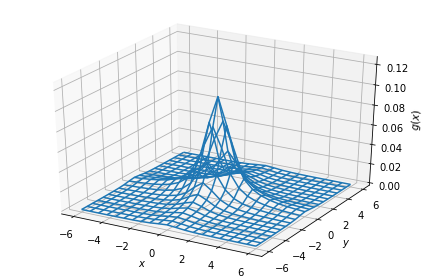
\includegraphics[width=0.4\linewidth]
		{figs/examplebvbmctrue.png}}
	\subfloat[Estimated density]{\label{fig11b}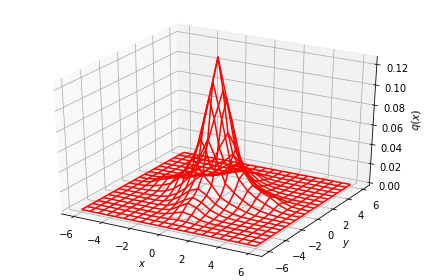
\includegraphics[width=0.4\linewidth]
	{figs/examplebvbmcestimated.png}}

	\caption[\label{bvbmcpackfigs}True density and estimated density found by running code in Figure \ref{bvbmcpackexample}]{\label{bvbmcpackfigs}True density (left) and estimated density (right), found by running code in Figure \ref{bvbmcpackexample}. Generating code can be found in \url{https://github.com/DFNaiff/Dissertation/blob/master/illustrations_dissertation/examplebvbmc.py}.}
\end{figure}

\chapter{Experiments}
In this chapter, BVBMC is applied in a number of examples, as to show the algorithm behavior in different scenarios. The examples consists of estimating continuous probability densities in up to $10$ dimensions \footnote{In more than $10$ dimensions, performance was very poor. What was seen is that the algorithm got \enquote{stuck} in its first component proposal, and could not find new components to be proposed with acceptable weights.}.

\section{1-d Mixture of Gaussians}

As a showcase example, a one-dimensional mixture of Gaussians is considered
\begin{displaymath}
 f(x) = \sum_{i=1}^{12} w_i \mathcal{N}(x;\mu_i,\sigma^2_i),
\end{displaymath}
with $w_i = \frac{1}{12}$, $\mu_i \sim \mathcal{N}(0,\sqrt{5})$ and $\sigma^2_i = 1$. This results in a many-peaked distribution, with mean $\mu_0=-1.6585$ and variance $\sigma^2_0 = 25.0316$, whose density is shown in Figure \ref{target1dmixture}. 

In each example, the quality of the approximation by the BVBMC algorithm is measured, by calculating both the difference between the estimated mean $\mu$ and the true mean $\mu_0$, in $\log_{10}|\mu - \mu_0|$, and the difference between the estimated variance $\sigma^2$ and the true variance $\sigma^2_0$, in $\log_{10}(|\sigma^2-\sigma^2_0|/|\sigma^2_0|)$. Code for this section can be found in \url{https://github.com/DFNaiff/Dissertation/tree/master/tests_dissertation/illustrative}. 

\begin{figure}
	\centering
	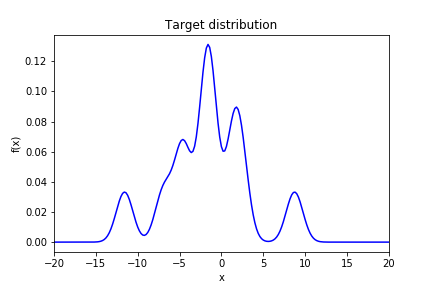
\includegraphics[width=0.7\linewidth]{figs/targetexil1a.png}
	\caption{\label{target1dmixture} Target distribution.}
\end{figure}

\subsection{Passive evaluation}
In the first two examples, the target evaluations of $\log f(x)$ were done in a uniform grid from $-20$ to $20$ with $51$ points, resulting in the GP replicating almost exactly the target distribution. This is done to illustrate the algorithm's capacity to generate good approximate distributions, if the GP approximates closely the (unnormalized) target distribution. Output scaling was done by normalizing, as discussed in Section \ref{outputscaling}. The GP mean was chosen to be constant, setting it with the heuristic corresponding to the \textit{normalize} scaling, as discussed in Section \ref{meansection}.

\subsubsection{Influence of kernel in approximation}
It was tested the kernel influence on the final approximation. For this, the tested kernels were $k_{\text{PMat},1/2}$, $k_{\text{PMat},2/2}$, $k_{\text{PMat},5/2}$ and $k_{\text{SQE}}$. The algorithm was run for 50 iterations, with joint parameter updating done every 10 steps. The results are shown in Figure \ref{kernelcomparison}.

There is an interesting behavior to be seen, in that the GP approximation for the kernels $k_{\text{PMat},1/2}$ and  $k_{\text{PMat},3/2}$ were considerably more accurate than with kernels $k_{\text{PMat},5/2}$ and $k_{\text{SQE}}$. However, this accuracy in the GP approximation does not reflect in a better posterior approximation, that are seen with $k_{\text{PMat},5/2}$ and $k_{\text{SQE}}$. This may be due to the fact that the first two kernels makes for GP approximations that are too rough, making it difficult to be approximated by the BVBMC algorithm.

\begin{figure}
	\centering
	\subfloat[$k_{\text{PMat},1/2}$, moments.]{\label{fig11a}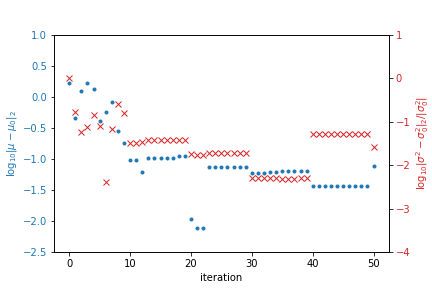
\includegraphics[width=0.4\linewidth]
		{figs/dmcil1fk12.png}}
	\subfloat[$k_{\text{PMat},1/2}$, final result.]{\label{fig11b}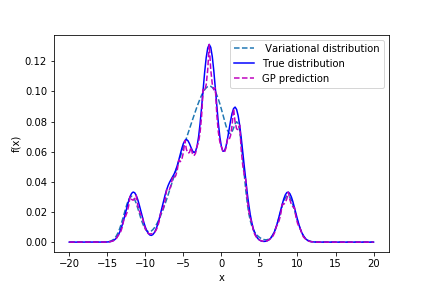
\includegraphics[width=0.4\linewidth]
	{figs/convgraphil1fk12.png}}

	\subfloat[$k_{\text{PMat},3/2}$, moments.]{\label{fig11a}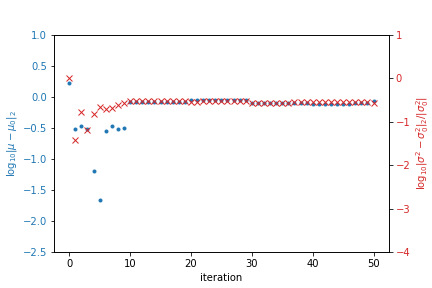
\includegraphics[width=0.4\linewidth]
	{figs/dmcil1fk32.png}}
\subfloat[$k_{\text{PMat},3/2}$, final result.]{\label{fig11b}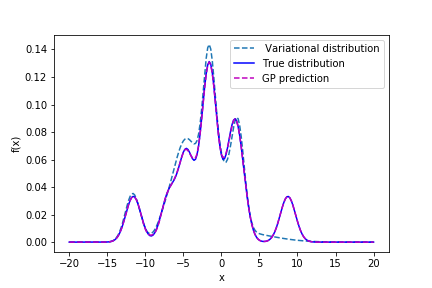
\includegraphics[width=0.4\linewidth]
	{figs/convgraphil1fk32.png}}

	\subfloat[$k_{\text{PMat},5/2}$, moments.]{\label{fig11a}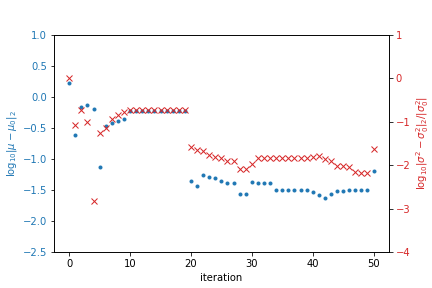
\includegraphics[width=0.4\linewidth]
	{figs/dmcil1fk52.png}}
\subfloat[$k_{\text{PMat},5/2}$, final result.]{\label{fig11b}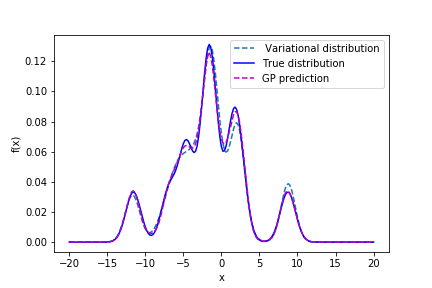
\includegraphics[width=0.4\linewidth]
	{figs/convgraphil1fk52.png}}

	\subfloat[$k_{\text{SQE}}$, moments.]{\label{fig11a}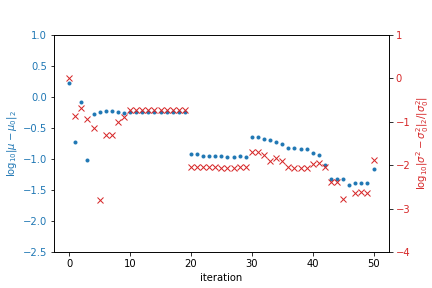
\includegraphics[width=0.4\linewidth]
	{figs/dmcil1fkSQE.png}}
\subfloat[$k_{\text{SQE}}$, final result.]{\label{fig11b}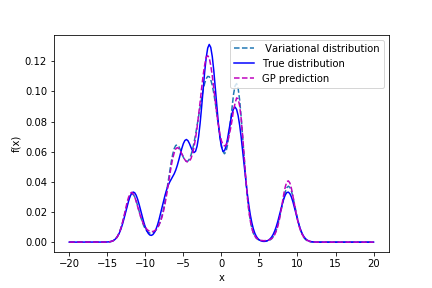
\includegraphics[width=0.4\linewidth]
	{figs/convgraphil1fkSQE.png}}
	\caption[Accuracy analysis for different kernels.]{\label{kernelcomparison} Accuracy analysis for different kernels. Each row corresponding to one kernel, in order being $k_{\text{PMat},1/2}$, $k_{\text{PMat},2/2}$, $k_{\text{PMat},5/2}$ and $k_{\text{SQE}}$. The first column (MC) shows the accuracy of mean (blue), and variance (red), while the second column shows the the predicted density, the true density and the GP approximation of the density.}
\end{figure}

\subsubsection{Influence of training routine in approximation}
Next, it was tested the difference that the training routine makes on both accuracy and algorithm running time. For this, using the same setting as above with kernel $k_{\text{PMat},5/2}$, three training routines were tested:
\begin{itemize}
	\item Running the algorithm for 50 iterations, with joint parameter updating done every step (training routine A).
	\item Running the boosting algorithm for 50 iterations, with joint parameter updating done every 10 steps (training routine B).
	\item Running the boosting algorithm for 50 iterations, with no joint parameter updating (training routine C).
\end{itemize}

The results are shown in Figure \ref{trainingcomparison}.  It can be seen that training routine B performs considerably better than routine A and routine C, while training routine A and training routine B has comparable final performance, with routine A converging in fewer iterations. As of running time, it can be see that for training routine A it increases quadratically in relation to the number of iterations, while for training routine C it increases linearly. As for training routine B, the running time increases linearly except to jumps corresponding to joint parameter updating, with each jump size growing with the iteration.

It is interesting to pause and consider the behavior of training routine B, since in the next set of examples this were the routine used, with some differences of number of iterations and intervals between joint parameter updating. Notice that boosting improves considerably accuracy up to the first joint parameter updating, in 10 iterations, and after this many intervals between two joint parameter updating essentially shows no improvements. This suggests that a smarter training routine, involving boosting only in the initial steps may be desirable. This idea was not explored further in this dissertation.

\begin{figure}
	\centering
	\subfloat[Routine A, moments]{\label{fig11a}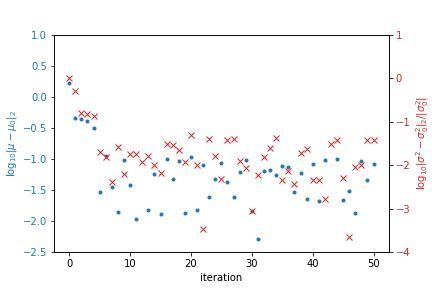
\includegraphics[width=0.35\linewidth]
		{figs/dmcil1ati1.png}}
	\subfloat[Routine A, final result.]{\label{fig11b}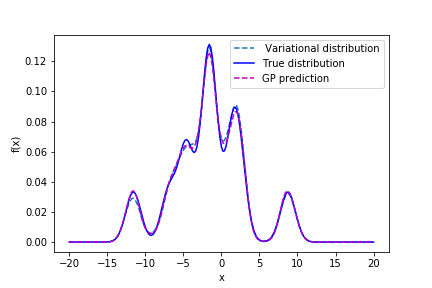
\includegraphics[width=0.35\linewidth]
		{figs/convgraphil1ati1.png}}
	\subfloat[Routine A, running time.]{\label{fig11b}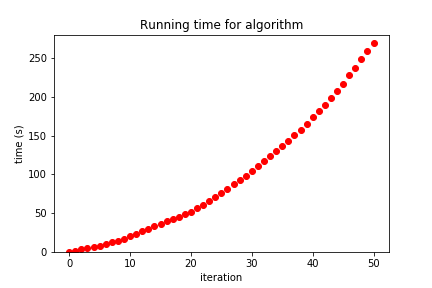
\includegraphics[width=0.35\linewidth]
	{figs/timegraphil1ati1.png}}

	\subfloat[Routine B,moments.]{\label{fig11a}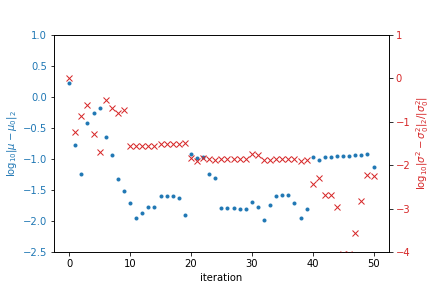
\includegraphics[width=0.35\linewidth]
		{figs/dmcil1ati10.png}}
	\subfloat[Routine B, final result.]{\label{fig11b}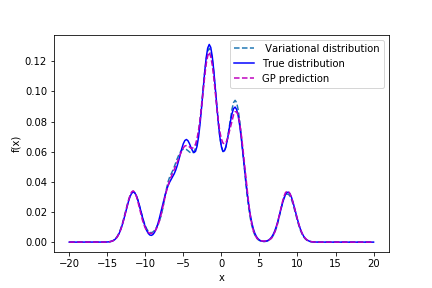
\includegraphics[width=0.35\linewidth]
		{figs/convgraphil1ati10.png}}
	\subfloat[Routine B, running time.]{\label{fig11b}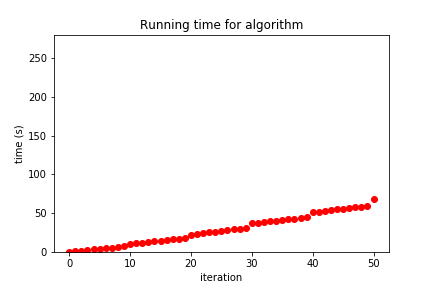
\includegraphics[width=0.35\linewidth]
	{figs/timegraphil1ati10.png}}

	\subfloat[Routine C, moments.]{\label{fig11a}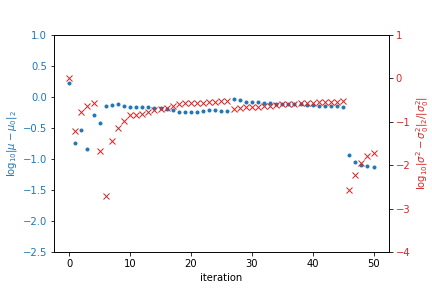
\includegraphics[width=0.35\linewidth]
		{figs/dmcil1ati1000.png}}
	\subfloat[Routine C, final result.]{\label{fig11b}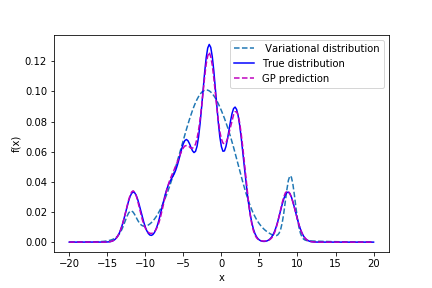
\includegraphics[width=0.35\linewidth]
		{figs/convgraphil1ati1000.png}}
	\subfloat[Routine C, running time.]{\label{fig11b}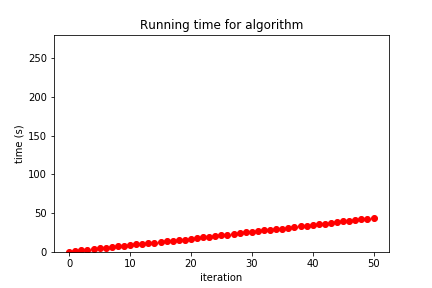
\includegraphics[width=0.35\linewidth]
	{figs/timegraphil1ati1000.png}}

	\caption[Accuracy analysis for different training routines.]{\label{trainingcomparison} Accuracy analysis for different training routines. Each row corresponding to training routine A, B and C, respectively. The first column shows the accuracy of mean (blue) and (red), the second column show the difference between the predicted density, the true density and the GP approximation of the density, and the third column shows the algorithm running time at each step.}
\end{figure}

\subsection{Active evaluation}
In this example, it is considered how BVBMC performs with active evaluation. For all examples, $5$ initial evaluation points are sampled randomly, with distribution $\mathcal{N}(0,\sqrt{10})$. Subsequently, at each iteration an evaluation point is chosen according to the running acquisition function. Four acquisition functions were tested: uncertainty sampling (US, \eqref{us_vbmc}), prospective prediction (PROP, \eqref{prospective_vbmc}), moment-matched log transform (MMLT, \eqref{mmlt_vbmc}), and prospective moment-matched log transform (MMLT$_P$, \eqref{mmltprop_vbmc}). The results are shown in Figure \ref{acquisition}. There it can be seen that all acquisition function performed well, although the GP approximation is better for the PROP and MMLT acquisitions.

\begin{figure}
	\centering
	\subfloat[US, moments.]{\label{fig11a}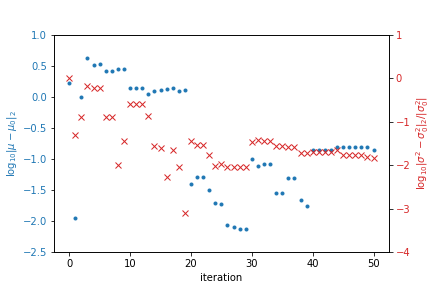
\includegraphics[width=0.35\linewidth]
		{figs/dmcil1g_aq_uncertainty_sampling.png}}
	\subfloat[US, final result.]{\label{fig11b}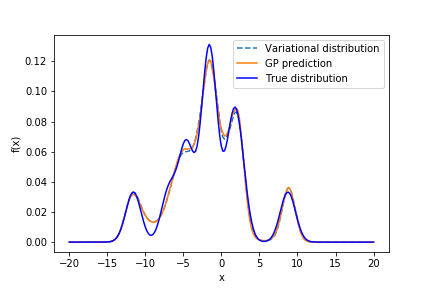
\includegraphics[width=0.35\linewidth]
		{figs/convgraphil1g_aq_uncertainty_sampling.png}}
	\subfloat[US, sampling.]{\label{fig11b}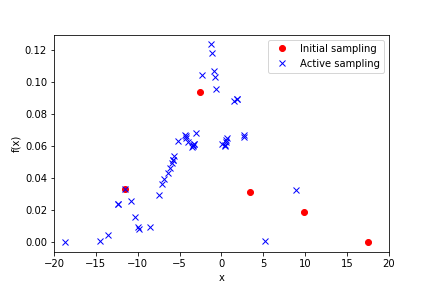
\includegraphics[width=0.35\linewidth]
		{figs/explopattern1g_aq_uncertainty_sampling.png}}
	
	\subfloat[PROP, moments.]{\label{fig11a}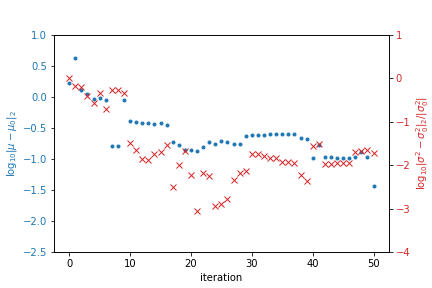
\includegraphics[width=0.35\linewidth]
	{figs/dmcil1g_aq_prospective.png}}
\subfloat[PROP, final result.]{\label{fig11b}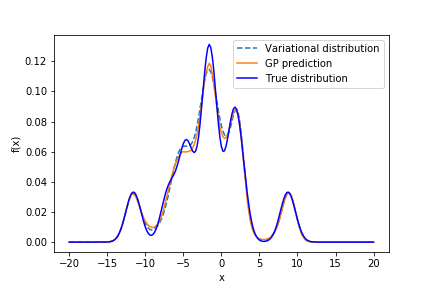
\includegraphics[width=0.35\linewidth]
	{figs/convgraphil1g_aq_prospective.png}}
\subfloat[PROP, sampling.]{\label{fig11b}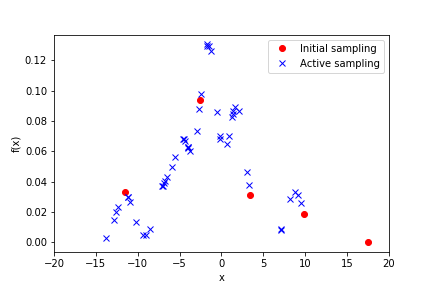
\includegraphics[width=0.35\linewidth]
	{figs/explopattern1g_aq_prospective.png}}
	
	\subfloat[MMLT, moments.]{\label{fig11a}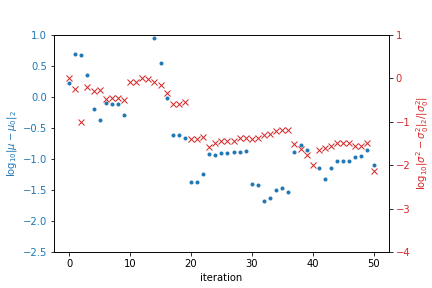
\includegraphics[width=0.35\linewidth]
	{figs/dmcil1g_aq_mmlt.png}}
\subfloat[MMLT, final result.]{\label{fig11b}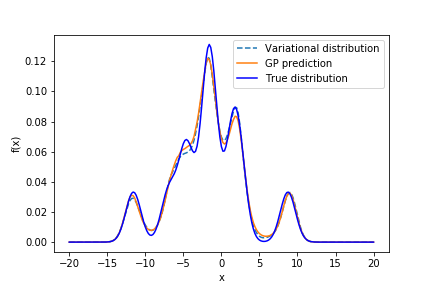
\includegraphics[width=0.35\linewidth]
	{figs/convgraphil1g_aq_mmlt.png}}
\subfloat[MMLT, sampling.]{\label{fig11b}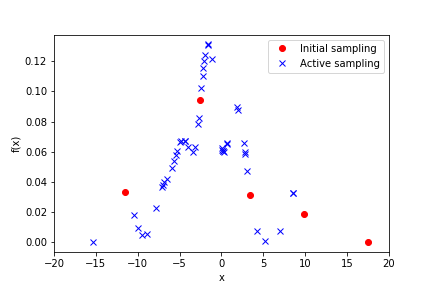
\includegraphics[width=0.35\linewidth]
	{figs/explopattern1g_aq_mmlt.png}}

	\subfloat[MMLT$_P$, moments.]{\label{fig11a}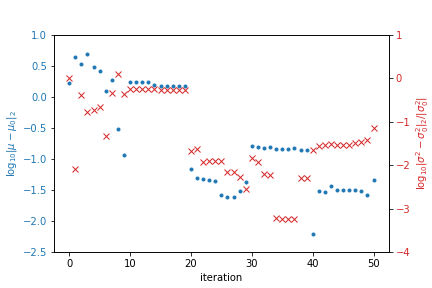
\includegraphics[width=0.35\linewidth]
	{figs/dmcil1g_aq_mmlt_prospective.png}}
\subfloat[MMLT$_P$, final result.]{\label{fig11b}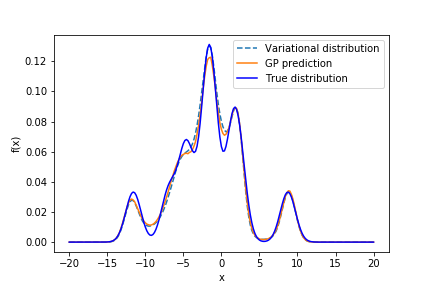
\includegraphics[width=0.35\linewidth]
	{figs/convgraphil1g_aq_mmlt_prospective.png}}
\subfloat[MMLT$_P$, sampling.]{\label{fig11b}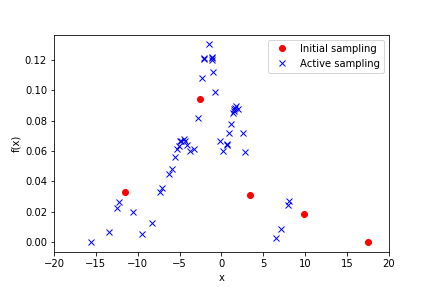
\includegraphics[width=0.35\linewidth]
	{figs/explopattern1g_aq_mmlt_prospective.png}}
	
	\caption[Accuracy analysis for different acquisition function.]{\label{acquisition} Convergence analysis for different acquisition function. Each row corresponds to acquisitions US, PROP, MMLT and MMLT$_P$, respectively. The first column shows the accuracy of mean and covariance, the second column show the difference between the predicted density, the true density and the GP approximation of the density, and the third column shows the places where the function was evaluated.}
\end{figure}

\newpage
\section{N-d toy examples}
In this section, we consider the algorithm performance on a set of toy examples, the same ones considered in \cite{Acerbi_2018}. Code for this section can be found in \url{https://github.com/DFNaiff/Dissertation/tree/master/tests_dissertation/toy}.

Three classes of test cases were considered:
\begin{itemize}
\item \textit{Lumpy}, a mixture of multivariate Gaussians
\begin{equation}
f(x) = \sum_{i=1}^{12} w_i \mathcal{N}(x;\mu_i,\Sigma_i),
\end{equation}
with $(w_1,\ldots,w_{12}) \sim \text{Dir}(1,\ldots,1)$, $\mu_i \sim \text{Unif}([0,1]^D)$ and $\Sigma = \text{diag}(\sigma_1^2,\ldots,\sigma_n^2)$, with $\sigma_i^2 \sim \text{Unif}(0.2,0.6)$. This distribution tests the algorithm performance in presence of possible multimodalities.

\item \textit{Cigar}, a anisotropic Gaussian distribution
\begin{equation}
f(x) = \mathcal{N}(x;0,\Sigma),
\end{equation}
where $\Sigma = Q \Lambda Q^T$, with $\Lambda = (10.0,0.1,\ldots,0.1)$, and $Q$ sampled from the uniform measure in the special orthogonal group. This distribution tests the algorithm performance in presence of large anisotropy.

\item \textit{Student-t}, a product of t distributions 
\begin{equation}
f(x) =  \prod_{d=1}^D \mathcal{T}(x_i;\nu_i),
\end{equation}
with $\nu_i \sim \text{Unif}(2.5,2+0.5D)$. This distribution tests the algorithm performance in presence of heavy tails \footnote{For both \textit{Cigar} and \textit{Student-t}, BVBMC was applied to an unnormalized density.} \footnote{Originally, $\nu_i = 2.5$ for every $i$, which assured reasonably heavy tails at every dimension. However, for comparison with \cite{Acerbi_2018}, this later case is not shown here}.
\end{itemize}

For each case, dimensions $D = 2,6,10$ where tested, and the BVBMC algorithm was run for $100$ iterations, with $10D$ initial samples. The GP kernel used were $k_{\text{PMat},\nu=2.5}$, with active evaluation at each iteration, according to an acquisition function randomly chosen between the pair $(\alpha_\text{PROP},\alpha_\text{MMLT})$. Every 20 steps, joint parameter updating was done, and pruning was done at each iteration, with $\beta = 10^{-3}$.

The algorithm performance was compared by checking the divergence between the true mean $\mu_0$ and the estimated mean $\mu$, in $\log_{10}||\mu - \mu_0||_2$, and between the true covariance $\Sigma_0$ and estimated covariance $\Sigma$, in $\log_{10}||\Sigma - \Sigma_0||_F/||\Sigma_0||_F$, where $||\cdot||_F$ denotes the Frobenius norm. The results are shown in Figure \ref{ndtoy}. For comparison with results given by the VBMC algorithm, shown in \cite{Acerbi_2018}, the "Gaussianized" symmetric KL divergence (gsKL) between the true distribution and estimated distribution is computed, which is defined as the symmetric KL divergence between two multivariate distributions with mean and covariance equals to the true distribution and the estimated distribution, respectively \footnote{In \cite{Acerbi_2018}, what is done are 15 evaluations for each case, and the median is taken. A better approach here would be doing the same thing for BVBMC, however due to time constraints this couldn't be done.}. The results are shown in Table \ref{toytable}. There it can be seen that, in general performance between BVBMC and VBMC was comparable, excluding the experiment with the \textit{Cigar} distribution with $D=10$, in which VBMC performed much better, and $D=2$, in which BVBMC performed better. \footnote{It should be noted that the BVBMC algorithm have used fewer evaluations, namely $120$,$160$ and $200$ for $D=2,6,10$, respectively, than the VBMC algorithm, which used $200$,$400$,$600$, for $D=2,6,10$. In this toy example this doesn't make a large computational difference, however in applications where likelihood evaluation is expensive it does.}

\begin{table}[]
	\begin{tabular}{l|l|l|l|l|l|l|}
		\cline{2-7}
		& \multicolumn{2}{l|}{Lumpy} & \multicolumn{2}{l|}{Cigar} & \multicolumn{2}{l|}{Student-t} \\ \cline{2-7} 
		& BVBMC         & VBMC        & BVBMC         & VBMC        & BVBMC         & VBMC        \\ \hline
		\multicolumn{1}{|l|}{D=2}  & $3.12 \times 10^{-3}$        & $6.5 \times 10^{-4}$         & $8.12 \times 10^{-3}$           & $2.1 \times 10^{-1}$         & $2.9 \times 10^{-1}$          & $2.0 \times 10^{-3}$         \\ \hline
		\multicolumn{1}{|l|}{D=6}  & $6.59 \times 10^{-2}$         & $ 3.5 \times 10^{-2}$         & $5.56 \times 10^{-1}$           & $ 1.07 \times 10^{-1}$        & $1.14 \times 10^{-1}$           & $2.3 \times 10^{-1}$         \\ \hline
		\multicolumn{1}{|l|}{D=10} & $1.19 \times 10^{-1}$           & $ 4.2 \times 10^{-1}$         & $1.29 $           &  $ 1.0 \times 10^{-1}$        & $2.56 \times 10^{-1}$           & $ 2.7 \times 10^{-1}$        \\ \hline
	\end{tabular}
	\caption{gsKL divergence between true distribution and estimated distribution. The values for VBMC were taken from the graphs in \cite{Acerbi_2018}.}\label{toytable}
\end{table}

\begin{figure}
	\centering
	\subfloat[Lumpy, means accuracy.]{\label{fig11a}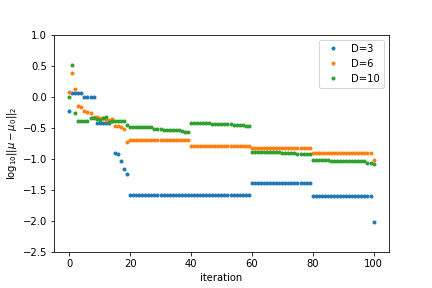
\includegraphics[width=0.5\linewidth]
		{figs/ex1b_mean.png}}
	\subfloat[Lumpy, covariances accuracy.]{\label{fig11b}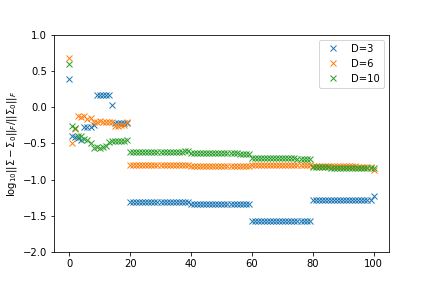
\includegraphics[width=0.5\linewidth]
		{figs/ex1b_cov.png}}

	
	\subfloat[Cigar, means accuracy.]{\label{fig11a}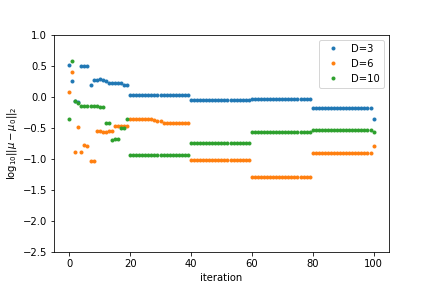
\includegraphics[width=0.5\linewidth]
		{figs/ex4b_mean.png}}
	\subfloat[Cigar, covariances accuracy.]{\label{fig11b}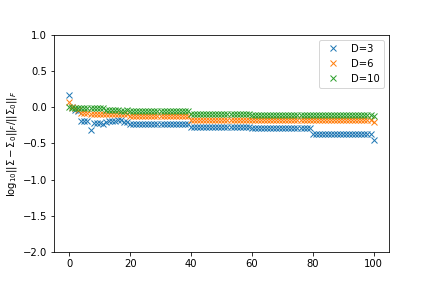
\includegraphics[width=0.5\linewidth]
		{figs/ex4b_cov.png}}

	\subfloat[Student-t, means accuracy.]{\label{fig11a}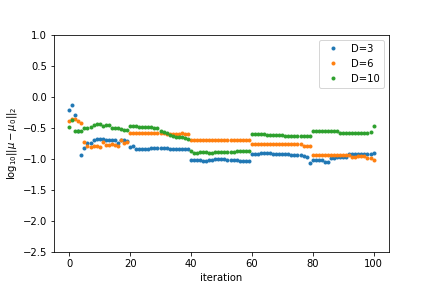
\includegraphics[width=0.5\linewidth]
	{figs/ex5b_mean.png}}
\subfloat[Student-t, covariances accuracy.]{\label{fig11b}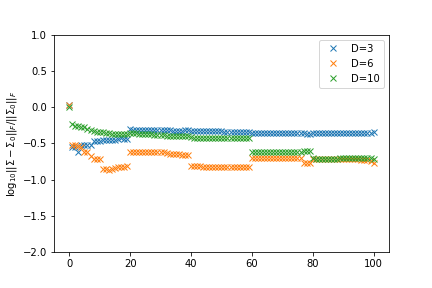
\includegraphics[width=0.5\linewidth]
	{figs/ex5b_cov.png}}

	
	\caption[Accuracy analysis for different N-d examples.]{\label{ndtoy} Accuracy analysis for different N-d examples. Each row corresponding to \textit{Lumpy}, \textit{Cigar} and \textit{Student-t}, respectively. The first column shows the accuracy of means, while the second column shows the accuracy of covariances.}
\end{figure}

\section{Contamination source estimation}
In this example, a contamination source location problem was considered, inspired by a problem in \cite{Bilionis_2013}. This problem is a toy example of an actual inverse problem, that is, given some sensor measurements of a contaminated field (the contamination may be, for instance, radiation), find where the contaminant as located, as well as its nature. Code for this section can be found in \url{https://github.com/DFNaiff/Dissertation/tree/master/tests_dissertation/source1d}.

The example consider a one-dimensional domain $B = [0,1]$, in which a contamination source $q(x,t)$ is inserted from $t=0$ to $t=t_s$. This source is modeled as
\begin{equation}
q(x,t) = q_0 \exp \left(-\frac{(x-x_0)^2}{2 \rho^2} \right) \mathbf{1}_{[0,t_s)}(t).
\end{equation}
The contaminant itself is assumed to follow the diffusion equation 
\begin{equation}
\frac{\partial}{\partial t} u(x,t) = \frac{\partial^2}{\partial x^2} u(x,t) + q(x,t), \quad x \in \text{int} B.
\end{equation}
Moreover, the initial contamination is considered to be $0$, while the walls are considered insulated, resulting in the boundary and initial value conditions
\begin{equation}
u(x,0) = 0, \; \frac{\partial}{\partial x} u(0,t) = \frac{\partial}{\partial x} u(1,t) = 0.
\end{equation}
It must be noticed that, for general domain length $L$ and diffusion coefficient $k$, using adimensionalization one can reduce the general problem to the above.

In this setting, at each wall $x=0,1$, four measurements of $u$ are made, for $t_m \in T_m = \{0.075,0.15,0.225,0.3,0.4\}$, resulting in the data 
\begin{displaymath}
 \mathcal{D} = \{\hat{u}(x_m,t_m)\}_{x_m \in \{0,1\},t_m \in T_m}.
\end{displaymath}
Moreover, the measurements are assumed to be noisy, with $\hat{u}(x_m,t_m) = u(x_m,t_m) + \epsilon$, $\epsilon \sim \mathcal{N}(0,\sigma^2)$. The noise parameter $\sigma^2$ is assumed to follow a prior $\text{InvGamma}(\alpha,\beta)$. This allows us to marginalize out $\sigma^2$, letting $\hat{u}(x_m,t_m)$ be distributed according to the generalized t-distribution \footnote{If $T_0$ follows a (standardized) t-distribution, with $nu$ degrees of freedom, then $T = \sigma T_0 + \mu$ follows a generalized t-distribution denoted by $\mathcal{T}(\mu,\sigma^2,\nu)$} with $2\alpha$ degrees of freedom $\mathcal{T}(u(x_m,t_m),\beta/\alpha,2 \alpha)$. 

The setting above results in a 4-dimensional inference problem, for the variables $(x_0,t_s,q_0,\rho)$, with likelihood
\begin{equation}
 p(\mathcal{D}|x_0,t_s,q_0,\rho) = \prod_{x_m \in \{0,1\},t_m \in T_M} \mathcal{T}(\hat{u}(x_m,t_m);u(x_m,t_m),\beta/\alpha,2 \alpha).
\end{equation}
Given priors for $x_0$,$t_s$,$q_0$ and $\rho$, the associated posterior distribution for the parameters becomes 
\begin{equation}\label{posteriorsource}
p(x_0,q_0,t_s,\rho|\mathcal{D}) \propto p(\mathcal{D}|x_0,q_0,T_s,\rho) p(x_0)p(q_0)p(\rho)p(t_s).
\end{equation}

A synthetic data $\mathcal{D}$ was generated, with the parameters given in Table \ref{sourcetable}, first row. The measurement noise was $\sigma^2 = 10^{-2}$, and the equation was simulated using a finite differences routine. The priors for the values to be inferred were set as \footnote{The Half-Cauchy distribution was used here as to represent a non-informative prior.}
\begin{equation}
\begin{split}
& p(x_0) = \text{Unif}(x_0;0,1) \\ 
& p(t_s) = \text{Unif}(t_s;0,0.4) \\
& p(q_0) = \text{HalfCauchy}(q_0;10) \\ 
& p(\rho) = \text{HalfCauchy}(\rho;0.1)
\end{split}
\end{equation}
In \eqref{posteriorsource}, $u(x,t)$ is also calculated by finite differences.

\begin{table}[h]
	\centering
	\begin{tabular}{l|l|l|l|l|}
		\cline{2-5}
		& $x_0$ & $t_s$ & $q_0$  & $\rho$ \\ \hline
		\multicolumn{1}{|l|}{True}  & 0.230 & 0.300 & 6.366  & 0.050  \\ \hline
		\multicolumn{1}{|l|}{BVBMC mean} & 0.328 & 0.213 & 5.435  & 0.140  \\ \hline
		\multicolumn{1}{|l|}{EMCEE mean} & 0.352 & 0.206 & 10.228 & 0.218  \\ \hline
		\multicolumn{1}{|l|}{BVBMC HDP 70\%} & $(1.1 \cdot 10^{-4},0.43)$ & $(0.12, 0.36)$ & $(1.0, 6.7)$ & $(2.7 \cdot 10^{-3}, 0.1)$  \\ \hline
		\multicolumn{1}{|l|}{EMCEE HDP 70\%} & $(3.4 \cdot 10^{-4}, 0.45)$ & $(0.08, 0.33)$ & $(0.4,10.3)$ & $(2.1 \cdot 10^{-3}, 0.1)$  \\ \hline
	\end{tabular}
	\caption{\label{sourcetable} Comparison of the true parameter of the problem (first row), the estimated means using BVBMC (second row) and EMCEE (third row), and 70\% highest posterior density interval for BVBMC and EMCEE.}
\end{table}

The BVBMC algorithm assumes that the distribution to be estimated has support in $\mathbb{R}^D$. This is not the case for the problem above, since $x_0$ and $t_s$ have both bounded support, while $q_0$ and $\rho$ have positive support. In order to apply the BVBMC algorithm, inference was made on the warped variables $\tilde{x}_0,\tilde{t}_s,\tilde{q}_0,\tilde{\rho}$, all of them with support in $\mathbb{R}$, such that  \footnote{The 0.4 factor here is due to the fact that $t_s$ lies between 0 and 0.4.}:
\begin{equation}
\begin{split}
 & x_0 = \text{sigmoid}(\tilde{x}_0) \\
 & t_s = 0.4 \times \text{sigmoid}(\tilde{t}_s)  \\
 & q_0 = \exp(\tilde{q}_0) \\
 & \rho = \exp(\tilde{\rho}), \\
\end{split}
\end{equation}
with
\begin{equation}
\text{sigmoid}(x) = \frac{1}{1+e^{-x}}.
\end{equation}
This results in the posterior distribution for the warped variables
\begin{equation}
 p(\tilde{x}_0,\tilde{t}_s,\tilde{q}_0,\tilde{\rho}|\mathcal{D}) \propto p(x_0,q_0,t_s,\rho|\mathcal{D}) \text{sigmoid}'(\tilde{x}_0) \text{sigmoid}'(\tilde{t}_s) \exp(\tilde{q}_0) \exp(\tilde{\rho})
\end{equation}

The BVBMC algorithm was applied to the problem, with the following setup:
\begin{itemize}
	\item The kernel used was $k_{\text{PMat},3/2}$ (both $k_{\text{PMat},5/2}$ and $k_{\text{SQE}}$ were also tested, with mixed results).
	\item The algorithm was initialized with 40 samples from the prior. After this, before the training loop, 40 more evaluations points were chosen by using the $\alpha_{MMLT}$ acquisition function.
	\item The algorithm was then run for 100 iterations, with an evaluation point chosen at each iteration, with the acquisition function chosen randomly between $\alpha_\text{{MMLT}}$ and $\alpha_\text{{PROP}}$. At each 20 iterations, the parameters were jointly optimized.
\end{itemize}

The predicted mean is shown in Table \ref{sourcetable}, second row. It can be seen that the estimated source location was relatively accurate, compared to the original one, while estimates for $\rho$ and $q_0$ where reasonable, and the estimate for $t_s$ did not deviate far from the prior mean. The resulting marginal univariate and bivariate distributions are shown in Figure \ref{sourcevbhistogram}.

\begin{figure}
	\centering
	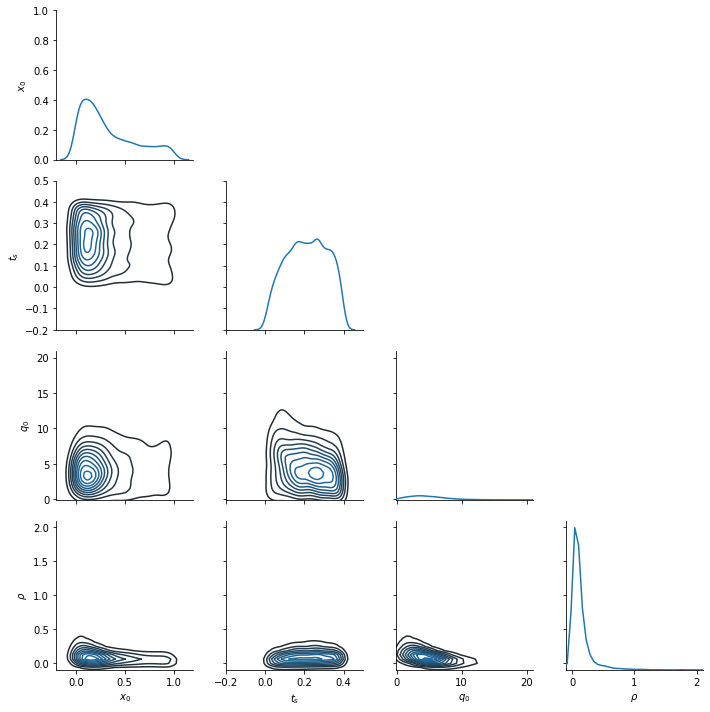
\includegraphics[width=0.8\linewidth]{figs/sourceproblemhistogramsvb.png}
	\caption[KDE plots of estimated marginals with BVBMC. On diagonal.]{KDE plots of estimated marginals with BVBMC. On diagonal, marginal univariate distributions for $x_0$,$t_s$,$q_0$ and $\rho$ are shown, while off-diagonal, the corresponding bivariate marginals for each pair is shown.}
	\label{sourcevbhistogram} 
\end{figure}

For comparison, the EMCEE algorithm \cite{Foreman_Mackey_2013}, which is a MCMC algorithm usually used for problems in astrophysics, was also tested. The EMCEE ran with $10$ walkers and $10000$ steps for each walker, using burn-in in the first $1000$ steps. The resulting estimated means is shown in Table \ref{sourcetable}, third row. It can be seem that in general the estimates were in the BVBMC algorithm, except for $q_0$, in which BVBMC seems to be more precise. The resulting marginal univariate and bivariate distributions are shown in Figure \ref{sourcevbhistogram}, showing some resemblance with the results found in BVBMC.

\begin{figure}
	\centering
	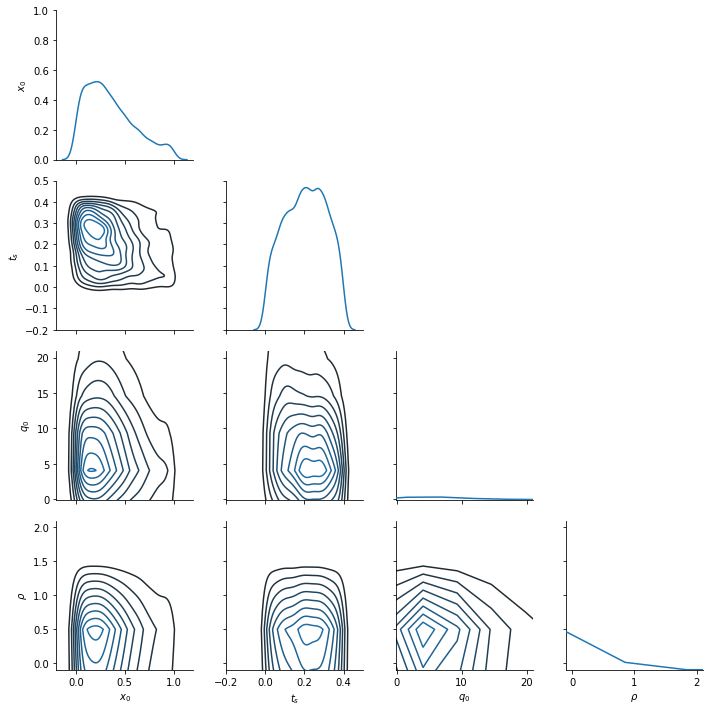
\includegraphics[width=0.8\linewidth]{figs/sourceproblemhistogramsemcee.png}
	\caption[KDE plots of estimated marginals with EMCEE. On diagonal.]{KDE plots of estimated marginals with EMCEE. On diagonal, marginal univariate distributions for $x_0$,$t_s$,$q_0$ and $\rho$ are shown, while off-diagonal, the corresponding bivariate marginals for each pair is shown.}
	\label{sourceemceehistogram} 
\end{figure}

\section{Checking performance}
In practice, one does not know the true posterior for doing comparison, and there must be some way to check whether BVBMC arrived at a good posterior.

Two sources of error may arise in the BVBMC estimate and the true posterior: Whether the variational proposal does not approximate well the GP surrogate model, or the GP surrogate model does not approximate well the true  unnormalized posterior. The first case may be checked using some rough estimate of the KL divergence between the variational proposal and the surrogate model, and is implemented in the method \textit{kl\_vb\_bmc} of the associated package. 

Checking whether the GP surrogate model resembles the true model may be harder. One option is to use leave-one-out testing \cite{Rasmussen06}, but one must consider that one does not care about accuracy in places where the unnormalized posterior does not contribute in probability mass. A heuristic to address this problem was not developed by the author.




\chapter{Future challenges and conclusion}
Here, we present some possible directions to extend the presented method to other applications.

\section{Reparameterization trick with Gaussian Processes}
The Bayesian Monte Carlo approach for approximating the integral terms
\begin{displaymath}
 \int \Ev[\log(\gu_\mathcal{D}(\theta))] q_i(\theta)
\end{displaymath}
suffers from the fact that the GP kernel and the distribution $q_i$ are limited, since
\begin{displaymath}
 \int k(\theta,\theta_i) q_i(\theta) d\theta
\end{displaymath}
must be tractable. One manner to circumvent this is by abandoning the BMC approach to integration, and insteading using the reparameterization trick presented in Section \ref{reparameterizationsection}, turning the BVBMC approach closer in spirit to the one in \ref{gradboostsection}.

One disadvantage is that evaluations of Gaussian Process, although cheap, are not extremely cheap, specially for large datasets, so reparameterization may be considerably slower.

\section{Extending BVBMC to pseudo-marginal likelihoods}
Consider that, as in Section \ref{pseudomarginalsection}, that $\gu(\theta) = Z p(\theta|\mathcal{D}) = p(\mathcal{D}|\theta) p(\theta)$ is truly unavailable, and even the pseudo-marginals $\hat{\gu}(\theta) = Z \hat{p}(\theta|\mathcal{D})$ are expensive to calculate.

Gaussian processes accommodates, for evaluation points $\{\theta_i\}_{i=1}^N$, the noisy estimates $\{\hat{\gu}(\theta_i)\}_{i=1}^N$ of $\{\gu(\theta_i)\}_{i=1}^N$. If one were doing GP regression on $\gu(\theta)$, one could assume that $p(\hat{\gu}|\gu)$ is roughly Gaussian, due to the central limit theorem, and use \eqref{meancovGPR} as surrogate model.

However, in BVBMC (and VBMC), one uses the GP surrogate model on $\log \gu(\theta)$. This implies that, letting $\epsilon = \hat{\gu}(\theta) - \gu(\theta)$ be the noise random variable, one have the model for $\log \bar{\gu}(\theta)$
\begin{equation}
 \log \bar{\gu}(\theta) = \log \left(e^{\log \gu(\theta)} + \epsilon \right),
\end{equation}
which is a complicated noise model, to be treated as in \eqref{generalnoise}. Furthermore, one cannot even assume this noise term to be controlled, since, by doing a rough Taylor expansion:
\begin{equation}
\log \bar{\gu}(\theta) = \log \gu(\theta) + e^{-\log \gu(\theta)} \epsilon
\end{equation}
which results in a very large noise for low values of $-\log \gu(\theta)$. One future work could be on how to address this problem.

\section{Scaling BVBMC to a larger number of evaluations}
Given the scaling problems of GP discussed in Section \ref{scalinggpsession}, for unnormalized posteriors $\gu(\theta)$ that can be evaluated in tens of thousands, but that evaluations in hundred of thousands or millions is hard, naive use of BVBMC runs into problems.

A possibility is two use sparse Gaussian Processes, that are briefly reviewed in the Appendix \ref{sparsegpchapter}. However, their integration with BVBMC ran into problems, so further research would be needed.

Of course, one could drop the use of GPs and use other surrogate function methods as done in \cite{Bliznyuk_2012,Marzouk_2007}. However, it should be noted that local approximation methods may not work with variational inference, because of its global approximation nature.

\section{Conclusion}
The method presented in this work, although still immature, has shown promise for use in Bayesian inference, where the likelihood function is expensive of evaluate, that are common in inverse problems.

The associated package in \url{https://github.com/DFNaiff/BVBMC}, built on top of PyTorch, is intended to be easy to use, so a practitioner can quickly employ it in their own problems, if they wish so.


 
%\chapter{Conclusion}

NOTA: ESTOU COM DIFICULDADE PARA ESSA CONCLUSAO.

The method presented in this work, although still immature, has shown promise for use in Bayesian inference, where the likelihood function is expensive of evaluate, that are common in inverse problems.

The associated package, built on top of PyTorch, is accessible and easy of use, and it is made so that a practitioner can quickly employ it in their own problems, if they wish so.           % Editar o arquivo introducao.tex

\bibliography{post-text/referencias}          % Editar o arquivo "referencias.bib"
\bibliographystyle{plain}

\clearpage

\appendix
%Obs.: No sistema operacional Windows, ao modificar este arquivo usando WinEdt, pode gerar erro do tipo:

%Error: Unicode char \u8: not set up for use with LaTeX.

%Se esse erro acontecer no WinEdt, modifique o Apêndice no Texmaker, rode nele e depois no WinEdt.


% Se não tiver Apêndice, deixar este arquivo em branco.

\chapter{SPARSE GAUSSIAN PROCESSES}\label{sparsegpchapter}

Given the scaling problem of GP methods, many sparsifications proposals were proposed, and the subject is a very fruitful area of research. We present below some of those approaches, although there are many other (for a recent review, see \cite{Haitao_2018}). In the following, $\sigma_n > 0$, for reasons that will be clear.

\section{Nystrom extension}
One approach is to simply approximate the matrix $K_\delta(\mathbf{x},\mathbf{x}) = K(\mathbf{x},\mathbf{x}) + \delta_n I$ in an manner that the matrix inversion (or Cholesky decomposition) becomes cheaper. One approach is to find an low-rank approximation of $K(\mathbf{x},\mathbf{x}) = U W U^T$, where $U$ is $n \times m$ and $W$ $m \times m$, and $m \ll n$. Then, one can find both the inverse and Cholesky decomposition of $V W V^T + \delta_n I$ with $\mathcal{O}(m^3)$ computational cost (\ref{matrixinversionlemma}).

The optimal $m$-rank approximation of $K(\mathbf{x},\mathbf{x})$, in both spectral norm and Frobenius norm is given by
\begin{displaymath}
\tilde{K} := \sum_{i=1}^l \lambda_i \mathbf{v}_i \mathbf{v}_i^T = V_l \Lambda_l V_l^T,
\end{displaymath} 
where $\lambda_1 \geq \ldots \geq \lambda_m \geq \lambda_{m+1} \geq \ldots \geq \lambda_n$ are the eigenvalues of $K(\x,\x)$, and $\mathbf{v}_1,\ldots \mathbf{v}_n$ are the corresponding eigenvalues (\cite{Eckart_1936}, coupled with the fact that for positive-semidefinite matrices the eigenvalue an singular value decomposition are the same). Then, $||K(\x,\x) - \tilde{K}||_2 = \lambda_{m+1}$. Unfortunately, this optimal low-rank approximation itself requires calculating the spectral decomposition of $K(\x,\x)$, which by itself has $\mathcal{O}(N^3)$ cost. So one has instead to find some cheap method to calculate a reasonable low-rank approximation of $m$.

The technique of Nystrom extensions was first introduced in \cite{Williams01usingthe}, and has found applications in kernel methods, as seen in \cite{Fowlkes_2004}, \cite{Wang_2009}. A $m$-rank Nystrom extension of a matrix $A$ $n \times n$ is formed by selecting $m$ (ordered) sub-indices from $\{1,\ldots,n\}$ (call it $I$), and then by letting $C$ be the $n \times m$ matrix formed by selecting the corresponding columns of $A$ and $W$ be the $m \times m$ matrix formed by selecting the intersection between the corresponding columns and corresponding rows of $A$, that is, 
\begin{displaymath}
C_{i,j} = A_{i,I_j}, \quad W_{i,j} = A_{I_i,I_j}.
\end{displaymath}
Then the corresponding Nystrom extension $\tilde{A}$ of $A$ is given by $A = C W^\dagger C^T$, where $W^\dagger$ is the pseudo-inverse of $W$. The simplest Nystrom extension technique is the naive Nystrom extension, where the $m$ sub-indices randomly without replacement from $\{1,\ldots,m\}$. With high probability, the optimal rank $k$ approximation of $A$ can be obtained by choosing $m = \mathcal{O}(k \log k)$ \cite{Gittens_2011}. In particular, if the spectrum of $A$ decays quickly, the naive Nystrom extension will result in a good low-rank approximation. This is usually the case for the kernel matrix $K(\x,\x)$, thus making this technique an attractive choice  at first. However, when applied to GP regression, one problem is that the predicive variance is not guaranteed to be positive, thus making the use of the Nystrom extension problematic \cite{Candela_2005}. Still, many sparsification techniques such as the ones shown below, end up using a version of it, with some correction ensuring that the posterior prediction is a valid distribution.


\section{Prior approximations}
The idea of prior approximations for sparsification of Gaussian Process is an unified view given by \cite{Candela_2005} that includes previous approaches offered in \cite{Smola_2001,Seeger_2003,Snelson_2006} To understand it, first note that one can over (dropping $M$ for convenience) an alternative derivation of the distribution for $p(\mathbf{f}^*|\mathbf{y})$ given in section 2.1, by expanding: 
\begin{equation} \label{GPRalternative}
p(\mathbf{f}^*|\mathbf{y}) = \int p(\mathbf{f},\mathbf{f}^*|\mathbf{y}) d \mathbf{f} 
= \frac{1}{p(\mathbf{y})} \int p(\mathbf{y}|\mathbf{f}) p(\mathbf{f},\mathbf{f}^*) d \mathbf{f}.
\end{equation} 
With the prior $p(\mathbf{f},\mathbf{f}^*)$ given by \eqref{jointGP}, assuming $m = 0$ for simplicity. Then, as shown in \ref{alternativegpsection}, one arrives at the exact same equation in \eqref{meancovGPR}. Then, since the matrix $K_{f,f}$ comes from $p(\mathbf{f},\mathbf{f})$, one approach to reduce the costs of its inverse is to approximate it.

To construct those approximations, first consider some new fictitious evaluation points, called \textit{inducing points} $\mathbf{x}_u = (x_{u,1},\ldots,x_{u,m})$, that may or may not include the training points, and the corresponding evaluations $\mathbf{u} = (f(x_{u,1}),...,f(x_{u,m}))^T$. Now, given the inducing points, one can write 
\begin{equation}
p(\mathbf{f},\mathbf{f}^*) = \int p(\mathbf{f},\mathbf{f}^*|\mathbf{u}) p(\mathbf{u}) d \mathbf{u},
\end{equation}
where $p(\mathbf{u}) = \mathcal{N}(\mathbf{u}|\mathbf{0},K_{u,u})$. Now, it is made the assumption that $\mathbf{f}$ and $\mathbf{f}^*$ are independent given $\mathbf{u}$, thus $p(\mathbf{f},\mathbf{f}^*|\mathbf{u}) \approx p(\mathbf{f}|\mathbf{u})p(\mathbf{f^*}|\mathbf{u})$. Without using further approximations for $p(\mathbf{f}|\mathbf{u})$ and $p(\mathbf{f^*}|\mathbf{u})$:
\begin{equation}
\begin{split}
& p(\mathbf{f}|\mathbf{u}) = \mathcal{N}(\mathbf{f}|K_{f,u} K_{u,u}^{-1} \mathbf{u}, K_{f,f} - K_{f,u} K_{u,u}^{-1} K_{u,f}) \\
& p(\mathbf{f}^{*}|\mathbf{u}) = \mathcal{N}(\mathbf{f}^{*}|K_{*,u} K_{u,u}^{-1} \mathbf{u}, K_{*,*} - K_{*,u} K_{u,u}^{-1} K_{u,*}).
\end{split}
\end{equation}
Using the notation $Q_{a,b} := K_{a,u} K_{u,u}^{-1} K_{u,b}$ and $K_{(f,*),u} := K((\mathbf{x},\mathbf{x}^*),\mathbf{u})$:
\begin{equation}
\left[ \begin{array}{c} 
\mathbf{f} \\

\mathbf{f^*} \end{array} \right] | \mathbf{u} \sim \mathcal{N} 
\left( \left[ \begin{array}{c}
K_{(f,*),u} (K_{u,u}+\sigma^2 I)^{-1} \mathbf{u} \end{array} \right] , 
\left[ \begin{array}{c c} 
K_{f,f} - Q_{f,f} & 0 \\
0 & K_{*,*} - Q_{*,*} \end{array} \right]
\right).
\end{equation}

By using the equation \ref{margingaussian}, we then find:
\begin{equation}\label{exactapproxinducing}
\begin{split}
\left[ 
\begin{array}{c} 
\mathbf{f} \\
\mathbf{f^*} 
\end{array}\right] \sim & \mathcal{N} 
\left( 0 , 
\left[ 
\begin{array}{c c} 
K_{f,f} - Q_{f,f} & 0 \\
0 & K_{*,*} - Q_{*,*} 
\end{array} \right] + K_{(f,*),u} K_{u,u}^{-1} K_{(f,*),u}^T
\right). \\
& \mathcal{N} 
\left( 0 , 
\left[ 
\begin{array}{c c} 
K_{f,f} - Q_{f,f} + Q_{f,f}& Q_{f,*} \\
Q_{*,f} & K_{*,*} - Q_{*,*} + Q_{*,*}
\end{array} \right]\right).
\end{split}
\end{equation}

By using \eqref{exactapproxinducing} in \eqref{GPRalternative}, we get:
\begin{equation}
\mathbf{f}^*|\mathbf{y} \approx \mathcal{N}(\mathbf{f}|Q_{*,f}(K_{f,f} + \sigma^2 I)^{-1} \mathbf{y},K_{*,*} - Q_{*,f}(K_{f,f} + \sigma^2 I)^{-1} Q_{f,*}).
\end{equation}

Nothing is really gained by considering the exact posteriors $p(\mathbf{f}|\mathbf{u})$ and $p(\mathbf{f}^*|\mathbf{u})$, since  still have the inverse of $K_{f,f} + \sigma^2 I$. Thus, there is need for further approximations, in turn to simplify the covariance matrix of $\mathbf{f}|\mathbf{u}$, thus simplifying $K_{f,f} + \sigma^2 I$ into something manageable for inversion. The main approximations of this kind are shown below. Notice that if the inducing points $\x_u$ are a subset of $\x$, then $Q_{f,f}$ is in fact a Nystrom extension of $K_{f,f}$.


\subsubsection{Subset of regressors}
The subset of regressors approximation for GPs was first proposed in \cite{Smola_2001}, adapting an idea from \cite{Silverman_1985}. It originally considered the generative model for \text{any} $\f^*$ (including the training values $\f$):
\begin{equation}
\f^* = K_{*,u} \mathbf{w}_u, \quad \mathbf{w}_u \sim \mathcal{N}(0,K^{-1}_{u,u}).
\end{equation}
In particular, this implies that $\u = K_{u,u} \mathbf{w}_u$, hence, within the prior approximation framework, the SoR technique approximates $\mathbf{f}|\mathbf{u}$ and $\mathbf{f}^*|\mathbf{u}$ by deterministic functions of their means, that is:
\begin{equation}
\begin{split}
& p(\mathbf{f}|\mathbf{u}) \approx q_{SoR}(\mathbf{f}|\mathbf{u}) = \mathcal{N}(\mathbf{f}|K_{f,u} K_{u,u}^{-1} \mathbf{u},0) \\
& p(\mathbf{f}|\mathbf{u}) \approx q_{SoR}(\mathbf{f}^*|\mathbf{u}) = \mathcal{N}(\mathbf{f}^{*}|K_{*,u} K_{u,u}^{-1} \mathbf{u},0).
\end{split}
\end{equation}
Then:
\begin{equation}
q_{SoR}(\mathbf{f},\mathbf{f}^*) = \mathcal{N} 
\left( 0 , 
\left[ 
\begin{array}{c c} 
Q_{f,f}& Q_{f,*} \\
Q_{*,f} & Q_{*,*}
\end{array} \right]\right),
\end{equation}
which results in the approximation $p(\mathbf{f}|\mathbf{y}) \approx q_{SOR}(\mathbf{f}|\mathbf{y})$:
\begin{equation}
q_{SOR}(\mathbf{f}^*|\mathbf{y}) = \mathcal{N}(\mathbf{f}|Q_{*,f}(Q_{f,f} + \sigma^2 I)^{-1} \mathbf{y},Q_{*,*} - Q_{*,f}(Q_{f,f} + \sigma^2 I)^{-1} Q_{f,*}).
\end{equation}

Since the marginal distribution of $\mathbf{f}$ is approximated by $\mathbf{Q_{f,f}}$, there is also an approximation for the likelihood of $\mathcal{D}$:
\begin{equation}
\log p(\mathcal{D}|M) \approx \log p(\mathbf{y}|M_{SoR},\mathbf{x}_u) = \log \mathcal{N}(\mathbf{y}|0,Q_{f,f} + \sigma^2 I).
\end{equation}
Notice that, since the matrix $Q_{f,f} = K_{f,u} K_{u,u}^{-1} K_{u,f}$ has low rank, one can use the matrix inversion lemma \ref{matrixinversionlemma} to calculate the inverse of $Q_{f,f} + \sigma^2 I$ with $\mathcal{O}(m^3)$ computational cost. If $m \ll n$, this gives a considerable gain in computation.

As noted in \cite{Smola_2001} subset of regressors approximation suffers from overconfident predictive variances, since the prior approximations for both training and testing points are degenerate, so caution must be taken with those.

\subsection{Deterministic Training Conditional}

The Deterministic Training Condition approximation, also called Projected Latent Variables when first proposed by \cite{Seeger_2003}, or Projected Process Approximation in \cite{Rasmussen06}, was originally proposed as a likelihood approximation for the training observations:
\begin{equation}
p(\y|\f) \approx \mathcal{N}(K_{f,u} K_{u,u}^{-1} \u, \sigma^2 I).
\end{equation}

In the prior approximation framework, an equivalent formulation can be made from by making a deterministic approximation the training points $\mathbf{f}|\mathbf{u}$, leaving $\mathbf{f}^*|\mathbf{u}$ unchanged, unlike the SoR method resulting in:
\begin{equation}
\begin{split}
& p(\mathbf{f}|\mathbf{u}) \approx q_{DTC}(\mathbf{f}|\mathbf{u}) = \mathcal{N}(\mathbf{f}|K_{f,u} K_{u,u}^{-1} \mathbf{u},0) \\
& p(\mathbf{f}|\mathbf{u}) \approx q_{DTC}(\mathbf{f}^*|\mathbf{u}) = \mathcal{N}(\mathbf{f}^{*}|K_{*,u} K_{u,u}^{-1} \mathbf{u},K_{*,*} - Q_{*,*}),
\end{split}
\end{equation}
resulting in the joint prior approximation:
\begin{equation}
q_{DTC}(\mathbf{f},\mathbf{f}^*) = \mathcal{N} 
\left( 0 , 
\left[ 
\begin{array}{c c} 
Q_{f,f}& Q_{f,*} \\
Q_{*,f} & K_{*,*}
\end{array} \right]\right),
\end{equation}
which results in the posterior approximation 
\begin{equation}\label{dtcprediction}
q_{DTC}(\mathbf{f}^*|\mathbf{y}) = \mathcal{N}(\mathbf{f}|Q_{*,f}(Q_{f,f} + \sigma^2 I)^{-1} \mathbf{y},K_{*,*} - Q_{*,f}(Q_{f,f} + \sigma^2 I)^{-1} Q_{f,*}),
\end{equation}
and the same data likelihood as in the subset of regressors case.
\begin{equation}\label{dtcobjective}
\log p(\mathcal{D}|M) \approx \log p(\mathbf{y}|M_{DTC},\mathbf{x}_u) = \log \mathcal{N}(\mathbf{y}|0,Q_{f,f} + \sigma^2 I)
\end{equation}

The DTC approximation improves considerably the predictive variances over the SoR approximation, while retaining the same predictive means. However, it has an inconsistency property in the fact that, for the training values $\f$, the covariance between then is computed differently whether they are considered as training values (in this case being $Q_{f,f}$) or as test values on the same points as the training points (being $K_{f,f}$), hence \cite{Candela_2005} claiming that it does not correspond exactly to a Gaussian Process. In practice, the advantage of it in relation of the DTC approximation compensates for this theoretical issue.


\subsection{Fully Independent Training Conditional and Fully Independent Conditional}

In the Fully Independent Training Conditional, originally proposed by \cite{Snelson_2006} with the name Sparse Gaussian Processes using Pseudo-Inputs, there is also an likelihood approximation as in the original formulations of the DTC approximation: 
\begin{equation}
p(\y|\f) \approx \mathcal{N}(K_{f,u}K_{u,u}^{-1} \u, \text{diag}(K_{f,f} - Q_{f,f}) + \sigma^2 I)
\end{equation}

In the prior approximation framework, the FITC approximates $p(\mathbf{f}|\mathbf{u})$ by the product of its marginal distributions, thus making an independence approximation for the training points, resulting in

\begin{equation}
p(\mathbf{f}|\mathbf{u}) \approx q_{FITC}(\mathbf{f}|\mathbf{u}) = \prod_{i=1} p(f_i|\mathbf{u}) = \mathcal{N}(\mathbf{f}|K_{f,u} K_{u,u}^{-1} \mathbf{u},\text{diag}(K_{f,f} - Q_{f,f})), 
\end{equation}
keeping $\f|\u$ unchanged as in the DTC approximation, 
resulting in the joint prior approximation:
\begin{equation}
q_{FITC}(\mathbf{f},\mathbf{f}^*) = \mathcal{N} 
\left( 0 , 
\left[ 
\begin{array}{c c} 
Q_{f,f} + \text{diag}(K_{f,f} - Q_{f,f})& Q_{f,*} \\
Q_{*,f} & K_{*,*}
\end{array} \right]\right),
\end{equation}
If there is only one evaluation point $\mathbf{f}^* = (\mathbf{f}_1)$, the FITC approximation can be seen as a diagonal correction of the DTC approximation for $p(\mathbf{f},\mathbf{f}^*|\mathbf{u})$. The FITC results in the posterior approximation
\begin{equation}\label{fitcpred}
\begin{split}
q_{FITC}(\mathbf{f}^*|\mathbf{y}) = \mathcal{N}(\mathbf{f}| Q_{*,f}(Q_{f,f} + D)^{-1} \mathbf{y}, K_{*,*} - Q_{*,f}(Q_{f,f} + D_f)^{-1} Q_{f,*}),
\end{split}
\end{equation}

Where $D_f := \sigma^2 I + \text{diag}(K_{f,f} - Q_{f,f})$. Hence the matrix inversion term is still tractable by the matrix inversion lemma. Finally, the likelihood approximation for $\mathbf{y}$ is given by:
\begin{equation}
\log p(\mathcal{D}|M) \approx \log p(\mathbf{y}|M_{FITC},\mathbf{x}_u) = \log \mathcal{N}(\mathbf{y}|0,Q_{f,f} + D_f).
\end{equation}

The FITC approximation also has the same inconsistency property as the DTC approximation. In \cite{Snelson_2006} it is proposed instead to approximate also the test points $\f^*|\u$ prior by $\prod_{i}  p(f^*_i|u)$, recovering the consistency property, resulting in the Fully Independent Conditional (FIC) approximation:

\begin{equation}
\begin{split}
q_{FIC}(\mathbf{f}^*|\mathbf{y}) = \mathcal{N}(\mathbf{f}|&Q_{*,f}(Q_{f,f} + D)^{-1} \mathbf{y}, \\
& Q_{*,*} + D_* - Q_{*,f}(Q_{f,f} + D_f)^{-1} Q_{f,*}),
\end{split}
\end{equation}
where $D_* := \text{diag}(K_{*,*} - Q_{*,*})$.
For a single test point, the FITC approximation and the FIC approximation returns exactly the same predictive distribution. In practice, the FITC approximation is used far more often than the FIC one.

\section{Posterior approximation via variational free energy}

Another popular approach to sparsification is given in \cite{Titsias_2009}, different in spirit from the ones presented above. To understand the idea of posterior approximations, consider:
\begin{equation}
p(\f^*|\y) = \int p(\f^*|\f) p(\f|\y) d \f
\end{equation}
We have 
\begin{equation*}
\begin{split}
p(\f|\y) & = \mathcal{N}(\f|K_{f,f}(K_{f,f} + \sigma^2 I)^{-1} \y,K_{f,f} - K_{f,f}(K_{f,f} + \sigma^2 I)^{-1} K_{f,f}) \\
& = \mathcal{N}(\f|\mu,A),
\end{split}
\end{equation*}
and
\begin{equation}
p(\f^*|\f) = \mathcal{N}(\f^*|K_{*,f}(K_{f,f} + \sigma^2 I)^{-1} \y,K_{*,*} - K_{*,f}(K_{f,f} + \sigma^2 I)^{-1} K_{f,*}).
\end{equation}
We then have, by \eqref{margingaussian}:
\begin{equation} \label{gpmarginy}
p(\f^*|\y) := \mathcal{N}(\f|K_{*,f}K^{-1}_{*,*} \mu,K_{*,*} - K_{*,f}(K_{f,f}^{-1}-K_{f,f}^{-1} A K_{f,f}^{-1}) K_{f,*}),
\end{equation}
which by the definition of $\mu$ and $A$ above yields the usual posterior distribution. 

Now consider again inducing point $\x_u$ with corresponding values $\f_u$, assuming that $\f$ and $\f^*$ are independent given $\f_u$. Notice that this implies $\f^*$ and $\y$ independent given $\f_u$, since $\y$ only depends on $\f$. Then, marginalizing on the inducing values:
\begin{equation}
p(\f^*|\y) \approx q(\f^*) =  \int p(\f^*|\f_u,\y) p(\f_u|\y) d\f_u = \int p(\f^*|\f_u) p(\f_u|\y) d\f_u.
\end{equation}
Therefore, changing $\f$ for $\f_u$, \eqref{gpmarginy} still holds. Since the true posterior $p(\f_u|\y)$ includes the inverse of $K_{f,f} + \sigma^2 I$, one option is to approximate $p(\f_u|\y)$ by a distribution $\phi(\f_u)$, also Gaussian with mean $\mu$ and covariance $A$, so that 
\begin{equation} \label{qumargin}
q(\f^*) = \int p(\f^*|\f_u) \phi(\f_u) = \int q(\f^*,\f_u),
\end{equation} 
in an manner that \eqref{gpmarginy} yields an sparse approximation.

One way to do this is to seek approximating the posterior $p(\f|\y)$ itself by some distribution $q(\f)$, involving $\phi(\f_u)$ on the training evaluations. As a proxy for this objective, the VFE method seeks to approximate the posterior for training and inducing values $p(\f,\f_u|\y)$ by $q(\f,\f_u)$, which, by \eqref{qumargin} is of form $q(\f,\f_u) = p(\f|\f_u) \phi(\f_u)$. Crucially, this augmented posterior depends on the inducing points $\x_u$ through $p(\f|\f_u)$, making then parameters of this approximate distribution, but not of the prior model $p(\f)$.

A natural way to find $q(\f,\f_u)$ is by minimizing the Kullback-Leibner divergence between $q(\f,\f_u)$ and $p(\f,\f_u|\y)$ 
\begin{displaymath}
KL(q(\f,\f_u)||p(\f,\f_u|\y) = - \int \int q(\f,\f_u) \log \frac{p(\f,\f_u|\y)}{q(\f,\f_u)} d\f d\f_u,
\end{displaymath}
which is equivalent to maximizing the evidence lower bound, or variational free energy (using $p(\f,\f_u|\y) \propto p(\y|\f) p(\f|\f_u) p(\f_u)$)
\begin{equation}
\begin{split}
F_V(q(\f,\f_u)) = F_V(\x_u,\phi) & = \int \int p(\f|\f_u) \phi(\f_u) \log \frac{p(\y|\f) p(\f|\f_u) p(\f_u)}{p(\f|\f_u) \phi(\f_u)} d \f d \f_u \\
& = \int \phi(\f_u) \left( \int p(\f|\f_u) \log p(\y|\f) d \f + \log \frac{p(\f_u)}{\phi(\f_u)} \right) d\f_m.
\end{split}
\end{equation}

This quantity is maximized by maximizing
\begin{equation}\label{vfeobjective}
F_V(\x_u) = \log \mathcal{N}(\mathbf{y}|0,Q_{f,f} + \sigma^2 I) - \frac{1}{2 \sigma^2} \text{tr}(K_{f,f} - Q_{f,f}),
\end{equation}
and setting $\phi(\f_u) = \mathcal{N}(\f_u|\mu^\dagger,A^\dagger)$, with
\begin{equation}\label{vfeobjective2}
\begin{split}
& \mu^\dagger = \sigma^{-2} K_{u,u} (K_{u,u} + \sigma^{-2} K_{u,f} K_{f,u})^{-1} K_{u,f} \y \\
& A^\dagger = K_{u,u} (K_{u,u} + \sigma^{-2} K_{u,f} K_{f,u})^{-1} K_{u,u}.
\end{split}
\end{equation}
The proof is given in \ref{vfemaxsection}. Substituting back in \eqref{gpmarginy}, we arrive at 
\begin{equation}\label{vfeprediction}
\begin{split}
& q_{VFE}(\f^*|\y) := \mathcal{N}(\f|\m_{VFE}^*,\Sigma_{VFE}^*) \\
& \m_{VFE}^* = \sigma^{-2} K_{*,u} (K_{u,u} + \sigma^{-2} K_{u,f} K_{f,u})^{-1} K_{u,f} \y \\
& \Sigma_{VFE}^* = K_{*,*} - Q_{*,*} + K_{*,u} (K_{u,u} + \sigma^{-2} K_{u,f} K_{f,u})^{-1} K_{u,*}.\\
\end{split}
\end{equation}
It can be show (\ref{vfeequipsection}) that these predictions correspond exactly to the DTC prediction. Thus, the VFE approach differs only in how the inducing points and kernel hyperparameters are trained, by maximizing \eqref{vfeobjective} instead of \eqref{dtcobjective}. Recent improvements of the VFE approach is be found in \cite{Bui_2016}, where an unification of the VFE and FITC approaches are proposed.

\subsection{Bayesian Monte Carlo with Sparse Gaussian Processes}

The extension for Bayesian Monte Carlo for the inducing points methods for sparsification presented in the previous section is straightforward. We will consider here only the FITC and the DTC approximations (being the case for the VFE approximation exactly the same as the DTC one). Considering $D = \sigma^2 I$ in the VFE approximation and $D = \sigma^2 I + \text{diag}(K_{f,f} - Q_{f,f})$ in the FITC one, by substituting the predictive mean and variance of \eqref{fitcpred} and \eqref{dtcprediction} in \eqref{evbmc} and \eqref{varbmc}, 
\begin{equation}
\begin{split}
& \Ev[Z_\mathcal{D}] = \mathbf{z}_u K_{u,u}^{-1} K_{u,f} (Q_{f,f} + D)^{-1} \y \\
& \Var[Z_{\mathcal{D}}] = \Gamma - \mathbf{z}_u^T K_{u,u}^{-1} K_{u,f} (Q_{f,f} + D) K_{f,u} K_{u,u}^{-1} \mathbf{z}_u,
\end{split}
\end{equation}
where
\begin{equation}
z_{u,i} = \int k(x,x_{u,i}) p(x) dx,
\end{equation}
and $\Gamma$ is the same as given in \eqref{varcoef}.

\subsection{VBMC and BVBMC with Sparse Gaussian Processes}
One of the techniques that was tried to expand the BVBMC method to wider applications was to use one of the sparse GP techniques shown here. However, it was found that, under low noise, the resulting matrices where very unstable, while when forcing artificially high noise, the results became innacurate.

It should be noted that, in that stage, only the SQE kernel was used, and it remains to be seen whether this problem still arises when using product of Matern kernels, which was a later development in this work.


\chapter{RELEVANT GAUSSIAN AND MATRIX IDENTITIES}

In the following, it is presented some relevant matrix and Gaussian distribution identities. All of those identities can be found in \cite{Petersen_2012}, except for \eqref{productgaussians}, which is slightly more general and can be found in \cite{Candela_2005}.
\section{Matrix inversion lemma}
If all the relevant inverses exists, then
\begin{equation}\label{matrixinversionlemma}
 (Z + UWV^T) = Z^{-1} - Z^{-1}U(W^{-1} + V^T Z^{-1} U)^{-1} V Z^{-1}.
\end{equation}
One consequence of the matrix inverse lemma is the formula
\begin{equation}\label{matrixinverselemmalemma}
\begin{split}
 (D + A)^{-1} & = (D + D D^{-1} A D^{-1} D)^{-1} = \\
			  & = (D - D^{-1} D ((D^{-1} A D^{-1})^{-1} + D D^{-1} D) D D^{-1})  = \\
			  & = D^{-1} - (D + D A^{-1} D)^{-1}.
\end{split}
\end{equation}
\section{Product of Gaussian densities}
\begin{equation}\label{productgaussians}
 \mathcal{N}(x|a,A) \mathcal{N}(Px|b,B) = z_c \mathcal{N}(x|c,C),
\end{equation}
where
\begin{displaymath}
 c = (A^{-1} + P B^{-1} P^T)^{-1}, \quad c = C(A^{-1}a + P^T B^{-1} b),
\end{displaymath}
and
\begin{displaymath}
 z_c = \mathcal{N}(Pa|b,B+P^T A P) = \mathcal{N}(b|Pa,B+P^T A P).
\end{displaymath}
In particular, this implies that
\begin{equation}\label{margingaussian}
 \int \mathcal{N}(b|Px,B) \mathcal{N}(x|a,A) dx = \mathcal{N}(b|Pa,B+P A P^T).
\end{equation}
\section{Conditional of a Gaussian density}\label{appendixconditional}
If
\begin{equation}
\left[ \begin{array}{c} 
\mathbf{x}_1 \\
\mathbf{x}_2 \end{array} \right] \sim \mathcal{N} 
\left( \left[ \begin{array}{c}
\mu_1 \\
\mu_2 \end{array} \right] , 
\left[ \begin{array}{c c} 
\Sigma_{11} & \Sigma_{12} \\
\Sigma_{21} & \Sigma_{22} \end{array} \right]
\right).
\end{equation}
then 
\begin{equation}
\mathbf{x}_1|\mathbf{x}_2 \sim \mathcal{N}\big(\mu_1 + \Sigma_{12} \Sigma_{22}^{-1}(\mathbf{x}_2 - \mu_2),\Sigma_{11} - \Sigma_{12}\Sigma_{22}^{-1} \Sigma_{21}\big).
\end{equation}
\clearpage

\chapter{Alternative derivation of GP predictions}\label{alternativegpsection}

Consider:
\begin{equation} \label{GPRalternativeAppendix}
p(\mathbf{f}^*|\mathbf{y}) = \int p(\mathbf{f},\mathbf{f}^*|\mathbf{y}) d \mathbf{f} 
= \frac{1}{p(\mathbf{y})} \int p(\mathbf{y}|\mathbf{f}) p(\mathbf{f},\mathbf{f}^*) d \mathbf{f}.
\end{equation}
By letting $P_f$ be the projection $(\mathbf{f},\mathbf{f}^*) \to \mathbf{f}$, and equivalently for $P_*$, and letting $K = K((\mathbf{x},\mathbf{x}^*),(\mathbf{x},\mathbf{x}^*))$, then
\begin{equation}
\begin{split}
 p((\f,\f^*|\y)) \propto p(\mathbf{y}|\mathbf{f}) p(\mathbf{f},\mathbf{f}^*) & = 
  \mathcal{N}(\y|\f,\sigma^2 I) \mathcal{N}((\f,\f^*)|0,K) \\
 & = \mathcal{N}(P_f(\f,\f^*)|\y,\sigma^2 I) \mathcal{N}((\f,\f^*|0,K)) \\
 & \propto \mathcal{N}((\f,\f^*)|c,C),
\end{split}
\end{equation}
where
\begin{equation}
 C = (K^{-1} + P_f^T \sigma^{-2} I P_f)^{-1}, \quad c = C P_f \sigma^{-2} \y.
\end{equation}
By the matrix inversion lemma
\begin{equation}
 C = K - K P_f^T (P_f K P_f^T + \sigma^2 I)^{-1} P_f K.
\end{equation}
Hence, by \eqref{margingaussian},
\begin{equation}
 p(\f^*|\y) = \mathcal{N}(\f|P_* c,P_* C P_*^T).
\end{equation}
We have for the posterior covariance
\begin{equation}
\begin{split}
 P_* C P_*^T & = P_* K P_*^T - P_* K P_f^T (P_f K P_f^T + \sigma^2 I)^{-1} P_f K P_* \\
 & = K_{*,*} - K_{*,f} (K_{f,f} + \sigma^2 I) K_{f,*},
 \end{split}
\end{equation}
and for the posterior mean
\begin{equation}
\begin{split}
 P_* c & = P_* K P_f \sigma^{-2} \y - P_* K P_f^T (P_f K P_f^T + \sigma^2 I)^{-1} P_f K P_f^T \y \\
 & = K_{*,f} (\sigma^{-2} I - (K_{f,f} + \sigma^2 I)^{-1} K_{f,f} \sigma^{-2} I) \y \\
 & = K_{*,f} (\sigma^{-2} I - (\sigma^2 I + \sigma^4 K_{f,f}^{-1})) \y \\
 & = K_{*,f} (K_{f,f} + \sigma^2 I)  \y.
 \end{split}
\end{equation}
where the last inequality comes from $\eqref{matrixinverselemmalemma}$ considering $D = \sigma^2 I$. Thus this derivation yields the same posterior distribution as in \eqref{meancovGPR}.

\chapter{Spectral mixture kernels and Bayesian Monte Carlo}
A kernel-distribution combination that yields analytical mean and variances for Bayesian Monte Carlo is the spectral mixture kernel in \eqref{spectralmixturekernel} combined with a Gaussian distribution $p(x) = \mathcal{N}(x|\mu,\Sigma)$ with diagonal covariance $\Sigma = \text{diag}(\sigma_1^2,\ldots,\sigma_D^{d})$, yielding 
\begin{equation}
\begin{split}
& z_i = \sum_{q=1}^Q w_q \prod_{d=1}^D \bigg[(2 \pi v_q^{(d)})^{-0.5} \cos\left(2 \pi C_{q}^{(d)} \mu_q^{(d)}(x_{i,d} - m_{d})\right) e^{-\pi (C_q^{(d)})^2 \mu_q^{(d)}} \\
& \qquad \qquad \qquad \qquad \mathcal{N}(x_{i,d}|m_d,(4\pi^2v_q^{(d)})^{-1}+\sigma_d^2)\bigg] \\
& \Gamma = \sum_{q=1}^Q w_q \prod_{d=1}^D \bigg[ (2 \pi v_q^{(d)})^{-0.5} e^{-\pi (C_q^{(d)})^2 \mu_q^{(d)}}
\exp\left(-\frac{1}{2} (A_q^{(d)} b_{q,d})^2 \right) (2\pi(\nu_{q,d}^2 + \sigma_d^2))^{-0.5}\bigg] \\
& \text{where} \quad C_{q}^{(d)} = (4 \pi v_q^{(d)} + \sigma_d^{-2})^{-1}, \, b_{q,d} = 2 \pi C_{q}^{(d)} \mu_q^{(d)} ,\, \\
& \qquad \qquad \nu_{q,d}^2 = (4\pi^2v_q^{(d)})^{-1}+\sigma_d^2 ,\, A_q^{(d)} = (\nu_{q,d}^{-2} + \sigma_d^{-2})^{-1}.
\end{split}
\end{equation}
This combination interesting because the spectral mixture kernel is far more flexible than the squared exponential one, thus enabling using Bayesian Monte Carlo to calculate expectations of more complex functions. Next it is shown the derivation for those formulas.

We will need first the result:
\begin{equation}
\begin{split}
& \int \cos(b(x-m)) \mathcal{N}(x|m,\nu^2) \mathcal{N}(x|\mu,\sigma^2) dx \\
& = \cos(C b (m - \mu)) \exp\left(-\frac{1}{2} C^2 b^2\right) \mathcal{N}(m|\mu,v^2 + \sigma^2) \\
& \text{where} \quad C = (\nu^{-2} + \sigma^{-2})^{-1}.
\end{split}
\end{equation}
To get it, use \eqref{productgaussians} in the integral, so it equals to:
\begin{equation*}
\begin{split}
& \mathcal{N}(m|\mu,\nu^2 + \sigma^2) \int \cos(b(x-m)) \mathcal{N}(x|c,C) dx = \\
& \mathcal{N}(m|\mu,\nu^2 + \sigma^2) \Re \left[\int e^{ib(x-m)} \mathcal{N}(x|c,C) dx \right] = \\
& \mathcal{N}(m|\mu,\nu^2 + \sigma^2) \Re \left[e^{-ibm} \int e^{ibx} \mathcal{N}(x|c,C) \right] = \\
& \mathcal{N}(m|\mu,v^2 + \sigma^2) \Re \left[e^{-ibm}e^{ibc - \frac{1}{2}C^2 b^2}\right] = \\
& \mathcal{N}(m|\mu,\nu^2 + \sigma^2) e^{-\frac{1}{2}C^2 b^2} \cos(b(c-m)), \\
& \text{where} \quad c = C (\nu^{-2} m + \sigma^{-2} \mu).
\end{split}
\end{equation*}
From the third to the fourth line above, we use the formula for the characteristic function of a Gaussian distribution. Finally, since $c - m = C(\nu^{-2}m+\sigma^{-2}\mu - C^{-1} m) = C\sigma^{-2}(\mu - m)$, and using the symmetry of cosine, the equality follows.

Letting $p(x) = \mathcal{N}(x|b,\text{diag}(\sigma_1^2,\ldots,\sigma_D^2))$ and $k(x,x_i) = k_{SM}(x - x_i)$:
\begin{equation}
\begin{split}
& \int k_{SM}(x - x_i) \mathcal{N}(x|m,\text{diag}(\sigma_1^2,\ldots,\sigma_D^2)) dx \\
& = \sum_{q=1}^Q w_q \int \left[\prod_{d=1}^D e^{-2 \pi^2 (x_d-x_{i,d})^2 v_{q}^{(d)}}
\cos(2 \pi (x_d-x_{i,d}) \mu_q^{(d)}) \prod_{d=1}^D\mathcal{N}(x_d|m_d,\sigma_d^2) dx_d \right] \\
&  = \sum_{q=1}^Q w_q \prod_{d=1}^D \int e^{-2 \pi^2 (x_d-x_{i,d})^2 v_{q}^{(d)}}
\cos(2 \pi (x_d-x_{i,d}) \mu_q^{(d)}) \mathcal{N}(x_d|m_d,\sigma_d^2) dx_d \\
& = \sum_{q=1}^Q w_q \prod_{d=1}^D (2 \pi v)^{-0.5}\int
\cos(2 \pi \mu_q^{(d)} (x_d-x_{i,d})) \mathcal{N}(x_d|x_{i,d},(4 \pi^2 v)^{-1})\mathcal{N}(x_d|m_d,\sigma_d^2) dx_d \\
& = \sum_{q=1}^Q w_q \prod_{d=1}^D (2 \pi v_q^{(d)})^{-0.5}\int
\cos(2 \pi \mu_q^{(d)} (x_d-x_{i,d})) \mathcal{N}(x_d|x_{i,d},(4 \pi^2 v)^{-1})\mathcal{N}(x_d|m_d,\sigma_d^2) dx_d \\
& = \sum_{q=1}^Q w_q \prod_{d=1}^D (2 \pi v_q^{(d)})^{-0.5} \cos\left(2 \pi C_{q}^{(d)} \mu_q^{(d)}(x_{i,d} - m_{d})\right) e^{-\pi (C_q^{(d)})^2 \mu_q^{(d)}} \mathcal{N}(x_{i,d}|m_d,(4\pi^2v_q^{(d)})^{-1}+\sigma_d^2) \\
& \text{where} \quad C_{q}^{(d)} = (4 \pi^2 v_q^{(d)} + \sigma_d^{-2})^{-1},
\end{split}
\end{equation}
and, letting $b_{q,d} = 2 \pi C_{q}^{(d)} \mu_q^{(d)}$ and $\nu_{q,d}^2 = (4\pi^2v_q^{(d)})^{-1}+\sigma_d^2$
\begin{equation}
\begin{split}
& \int \int k_{SM}(x_i - x_j) \mathcal{N}(x_i|\mu,\text{diag}(\sigma_1^2,\ldots,\sigma_D^2)) \mathcal{N}(x_j|\mu,\text{diag}(\sigma_1^2,\ldots,\sigma_D^2)) dx_i,dx_j\\
& = \sum_{q=1}^Q w_q \prod_{d=1}^D \bigg[(2 \pi v_q^{(d)})^{-0.5} e^{-\pi (C_q^{(d)})^2 \mu_q^{(d)}} \\ 
& \qquad \qquad \qquad \int \cos\left(b_{q,d}(x_{i,d} - m_{d})\right) \mathcal{N}(x_{i,d}|m_d,\nu_{q,d}) \mathcal{N}(x_{j,d}|m_d,\sigma_d^2)dx_{j,d} \bigg] \\
& = \sum_{q=1}^Q w_q \prod_{d=1}^D \bigg[ (2 \pi v_q^{(d)})^{-0.5} e^{-\pi (C_q^{(d)})^2 \mu_q^{(d)}} \exp\left(-\frac{1}{2} (A_q^{(d)} b_{q,d})^2 \right) (2\pi(\nu_{q,d}^2 + \sigma_d^2))^{-0.5}\bigg] \\
& \text{where} \quad A_q^{(d)} = (\nu_{q,d}^{-2} + \sigma_d^{-2})^{-1}.
\end{split}
\end{equation}

\chapter{Derivations for VFE}

\section{Maximizaton of variational free energy}\label{vfemaxsection}
For the integral inside parenthesis in \eqref{vfeobjective}, letting $\alpha = K_{f,u} K_{u,u} \f$ and $M = K_{f,f} - Q_{f,f}$, $p(\f|\f_u) = \mathcal{N}(\f|\alpha,M)$:
\begin{equation*}
\begin{split}
\int p(\f|\f_u) \log p(\y|\f) d\f & = 
\int p(\f|\f_u) \left[ -\frac{1}{2 \sigma^2} (\y - \f)^T (\y - \f) -\frac{d}{2} \log(2 \pi \sigma^2) \right] d \f \\
 & = -\frac{n}{2}  \log(2 \pi \sigma^2) - \Ev_{\f|\f_u}\left[\text{tr}\left(\frac{1}{2\sigma^2}(\f - \y)(\f - \y)^T\right)\right] \\
 & = -\frac{n}{2} \log(2 \pi \sigma^2) - \frac{1}{2\sigma^2} \text{tr}((\alpha-\y)(\alpha-\y)^T + A) = \\
 & = \log \mathcal{N}(\y|\alpha,\sigma^2 I) - \text{tr}(K_{f,f} - Q_{f,f}).
\end{split}
\end{equation*}
Substituing back in \eqref{vfeobjective}:
\begin{equation}\label{vfeobjectivepartial}
 F_V(\x_u,\phi) = \int \phi(\f_u) \log \frac{\mathcal{N}(\y|\alpha,\sigma^2 I) p(\f_u)}{\phi(\f_u)}d\f_u - \text{tr}(K_{f,f} - Q_{f,f}).
\end{equation}
For any $\x_u$ fixed, $F_V(\x_u,\phi)$ is then maximized by maximizing the integral term. But this is just the evidence lower bound between $\phi$ and the unnormalized distribution $\mathcal{N}(\y|\alpha,\sigma^2 I) p(\f_u)$, relative to $\f_u$. Without constraining $\phi$, then we must have:
\begin{equation}
\begin{split}
 \phi(\f) & \propto \mathcal{N}(\y|\alpha,\sigma^2 I) p(\f_u) \\
		  & \propto \exp \left( -\frac{1}{2 \sigma^2}(\y - \alpha)^T(\y - \alpha) -\frac{1}{2} \f_u^T K_{u,u} \f_u \right) \\
		  & \propto \exp\left(\frac{1}{\sigma^2}\y^T K_{f,u} K_{u,u}^{-1} \f_u - 
			  \frac{1}{2} \f_u^T \left(K_{u,u}^{-1} + 
			  \frac{1}{\sigma^2} K_{u,u}^{-1} K_{u,f} K_{f,u} K_{u,u}^{-1} \right) \f_u \right).
\end{split}
\end{equation}
The quadratic form can be completed relative to $\f_u$ to find:
\begin{equation}
\begin{split}
& A^\dagger = (K_{u,u}^{-1} + \sigma^{-2} K_{u,u}^{-1}K_{u,f}K_{f,u}K_{u,u}^{-1})^{-1} = K_{u,u}(K_{u,u} + \sigma^{-2} K_{u,f}K_{f,u})^{-1} K_{u,u} \\
& \mu^\dagger = \sigma^{-2} K_{u,u} (K_{u,u} + \sigma^{-2} K_{u,f} K_{f,u})^{-1} K_{u,f} \y.
\end{split}
\end{equation}
Since $\phi$ is itself Gaussian, the unconstrained optimum is the same as for the constrained one. Finally, since $\phi(\f) = \frac{1}{Z}\mathcal{N}(\y|\alpha,\sigma^2 I) p(\f_u)$, with $Z = \int \mathcal{N}(\y|\alpha,\sigma^2 I) p(\f_u) d\f_u$, substituting back into \eqref{vfeobjectivepartial}, we find the objective function for $\x_u$,
\begin{equation}
\begin{split}
 F_V(\x_u) & = \log \int \mathcal{N}(\y|K_{f,u} K_{u,u} \f,\sigma^2 I) \mathcal{N}(0,K_{u,u}) d\f_u - \text{tr}(K_{f,f} - Q_{f,f}) \\
 & = \log \mathcal{N}(\y|0,Q_{f,f} + \sigma^2 I) - \text{tr}(K_{f,f} - Q_{f,f}).
 \end{split}
\end{equation}
\section{Equivalence between VFE and DTC prediction}\label{vfeequipsection}

Starting with \eqref{vfeprediction}, for the covariance, we use the matrix inversion lemma, by letting $\Delta = \sigma^2 I$:
\begin{equation*}
\begin{split}
 & K_{*,u}(K_{u,u} + K_{u,f} \Delta^{-1} K_{f,u})^{-1} K_{u,*} = \\
 & K_{*,u}(K_{u,u}^{-1} - K_{u,u}^{-1} K_{u,f} (K_{f,u} K_{u,u}^{-1} K_{u,f} + \Delta)^{-1} K_{f,u} K_{u,u}^{-1}) K_{u,*} = \\
 & Q_{*,*} - Q_{*,f}(Q_{f,f} + \Delta)^{-1} Q_{f,*}.
\end{split}
\end{equation*}
Substituting in the covariance term for \eqref{vfeprediction}, we find the same covariance as in \eqref{dtcprediction}. For the mean term, using again the matrix inversion lemma, we find:
\begin{equation*}
\begin{split}
& K_{*,u} (K_{u,u} + K_{u,f} \Delta^{-1} K_{f,u})^{-1} K_{u,f} \Delta^{-1} \y = \\
& K_{*,u} (K_{u,u}^{-1} - K_{u,u}^{-1} K_{u,f} (K_{f,u} K_{u,u}^{-1} K_{u,f} + \Delta)^{-1} K_{f,u} K_{u,u}^{-1}) K_{u,f} \Delta^{-1} \y = \\
& (Q_{*,f} - Q_{*,f}(Q_{f,f} + \Delta)^{-1} Q_{f,f}) \Delta^{-1} \y = \\
& Q_{*,f}(\Delta^{-1} - (Q_{f,f} + \Delta)^{-1} Q_{f,f} \Delta^{-1} )\y = \\
& Q_{*,f}(\Delta^{-1} - (\Delta Q_{f,f}^{-1})(Q_{f,f} + \Delta))^{-1} \y = \\
& Q_{*,f}(\Delta^{-1} - (\Delta + \Delta Q_{f,f}^{-1} \Delta)^{-1}) \y = \\
& Q_{*,f}(Q_{f,f} + \Delta)^{-1} \y,
\end{split}
\end{equation*}
where in the last equality it was used \eqref{matrixinverselemmalemma}. This is the same mean term as in \eqref{dtcprediction}, thus proving the equality.
\chapter{REINFORCE gradient}
We have that
\begin{equation}
\begin{split}
& \nabla \Ev_{q(\theta;\lambda)}\left[\log \left(\frac{\gu(\theta)}{q(\theta;\lambda)}\right)\right] \\& = \nabla \int \log \left(\frac{\gu(\theta)}{q(\theta;\lambda)}\right) q(\theta;\lambda) d\theta \\
& = \int \nabla_\lambda \left( \log \left( \frac{\gu(\theta)}{q(\theta;\lambda)}\right) q(\theta;\lambda) \right) d\theta \\
& = \int q(\theta;\lambda) \nabla_\lambda \log q(\theta;\lambda) d\theta + \int \log \left( \frac{\gu(\theta)}{q(\theta;\lambda)}\right) \nabla_\lambda q(\theta;\lambda) d\theta
\end{split}.
\end{equation}
The first term in the sum equals to
\begin{equation}
\begin{split}
\int q(\theta;\lambda) \nabla_\lambda \log q(\theta;\lambda) d\theta & = \int q(\theta;\lambda) \frac{\nabla_\lambda q(\theta;\lambda)}{q(\theta;\lambda)} d\theta \\
& = \nabla \int q(\theta;\lambda) d\theta \\
& = \nabla 1 = 0,
\end{split}
\end{equation}
while the second term equals to
\begin{equation}
\begin{split}
& \int \log \left( \frac{\gu(\theta)}{q(\theta;\lambda)}\right) \nabla_\lambda q(\theta;\lambda) d\theta \\ & = \int \log \left( \frac{\gu(\theta)}{q(\theta;\lambda)}\right) \nabla_\lambda ( \log q(\theta;\lambda)) q(\theta;\lambda) d\theta \\
& = \Ev_{q(\theta;\lambda)} \left[ \log \frac{\gu(\theta)}{q(\theta;\lambda)} \nabla_{\lambda} \log q(\theta;\lambda) \right]
\end{split}
\end{equation}
Joining the two terms, we arrive at \eqref{reinforce}.
          % Editar o arquivo apendice.tex

\end{document}

%\citep* - citação completa, com todos os autores

%\citeyearpar - cita somente o ano da publicação
chapters